\documentclass[12pt]{kththesis}


\titleformat
{\chapter}
[display]
{\normalfont\Large\bfseries}
{Kapitel \thechapter}
{0.5ex}
{}
[]



\usepackage{blindtext} % This is just to get some nonsense text in this template, can be safely removed

\usepackage[parfill]{parskip}
\usepackage{caption}
\usepackage{multirow}
\usepackage{pdfpages}
\usepackage{graphicx}
\usepackage[title,toc,page]{appendix}
\graphicspath{ {./images/} }
\usepackage{mathtools}
\usepackage{csquotes} % Recommended by biblatex
\usepackage{biblatex}
\usepackage{times}
\usepackage{afterpage}

\usepackage{fancyhdr}

% Defining the new page style
\pagestyle{fancy}
\fancypagestyle{MyStyle}{%
    \fancyhead{} %Clean headers
    \fancyhead[RO]{\leftmark}
    \fancyhead[LE]{\leftmark}
    \renewcommand{\chaptermark}[1]{\markboth{\thechapter. {\slshape{##1}}}{}}
} 
\addbibresource{references.bib} % The file containing our references, in BibTeX format


\title{This is the English title}
\alttitle{Detta är den svenska översättningen av titeln}
\author{Osquar Studnt}
\email{osquar@kth.se}
\supervisor{Lotta Larsson}
\examiner{Lennart Bladgren}
\programme{Master in Computer Science}
\school{School of Electrical Engineering and Computer Science}
\date{\today}

\DeclareUnicodeCharacter{2217}{-}
\begin{document}
\renewcommand\appendixname{Appendix}
\renewcommand\appendixpagename{Appendix}
\renewcommand\appendixtocname{Appendix}
\pagestyle{MyStyle}


% Frontmatter includes the titlepage, abstracts and table-of-contents
\frontmatter
\afterpage{\null\newpage}


\includepdf[pages={-}]{StartPage.pdf}
\afterpage{\null\newpage}

\includepdf[pages={-}]{Titlepage.pdf}
\begin{otherlanguage}{swedish}
  \begin{abstract}
\afterpage{\null\newpage}

I dagsläget finns det en mängd utmaningar och svårigheter inom den traditionella designprocessen för UX, User Experience. Dessa utmaningar har en påverkan på hur tidskrävande och kostsam en designprocess för UX kan vara. Några av dem är att få prototyper att likna slutprodukten och kommunikationssvårigheter mellan UX-designers och utvecklare vid Agil projektmetodik. Det finns även svårigheter vid visualisering av strömmande data då informationen i data ska göras lättförståelig för användaren och att möjliggöra användaren att nå önskad information.

För att undersöka dessa svårigheter togs en designprocess för UX, att användas med datavisualiseringsverktyget Kibana, fram. För att kunna utvärdera och bedöma designprocessen för UX, skapades en interaktiv \textit{dashboard} som presenterade Transportstyrelsens data från betalstationer. Efter framtagningen av designprocessen för UX konstaterades det att prototypskapandet och testningen optimerades. Fördelar med att använda Kibana var att designprocessen hade fokus på produkten och inte prototypen vilket förbättrade testningen med slutanvändaren och därmed även slutprodukten. Det fanns dock nackdelar då Kibana användes vilka var begränsningar i modifiering av användargränssnittet och att systemet behövde vara klart innan designprocessen för UX kunde påbörjas. 


\textbf{Nyckelord}

\textit{Kibana, Elastic Stack, UX-designprocess, UX, Användarupplevelse}

 \end{abstract}
\end{otherlanguage}
 
\afterpage{\null\newpage}

\begin{abstract}

In the current situation there are a lot of challenges and difficulties in the traditional design process for UX, User Experience. These challenges have an impact on how time consuming and costly a design process for UX can be. Some of them are to create prototypes that resemble the end product and communication difficulties between UX-designers and developers that follow an Agile project methodology. There are also difficulties in visualizing streaming data, as information in data must be made easy to understand for the user and to enable the user to get desired information.
 
To investigate these difficulties, a design process for UX was created to be used with the Kibana data visualization tool. In order to evaluate and assess the design process for UX, an interactive \textit{dashboard} was created that presented data from Swedish payment stations. After developing the design process for UX, it was found that prototype creation and testing were optimized. The advantages of using Kibana were that the design process focused on the product and not the prototype, which improved the testing with the end user and therefor also the end product. However, there were disadvantages when Kibana was used which were limitations in modifying the user interface and that the system needed to be ready before the UX design process could begin.


\textbf{Keywords}

\textit{Kibana, Elastic Stack, UX-design process, UX, User Experience}

\end{abstract}

\chapter*{Förord}
Detta projekt är ett resultat av ett examensarbete inom datateknik på Kungliga Tekniska Högskolan, på uppdrag av företaget ÅF Digital Solutions AB. Arbetet har utförts av Christina Ntis och Neira Causevic på heltid under perioden mars 2018 - juni 2018.

Text som är i kursiv stil i denna rapport är termer på engelska som inte var lämpliga för översättning till svenska.

Vi skulle vilja tacka alla inblandade parter i detta examensarbete på ÅF och KTH. Stort tack till Martin Neumann, vår handledare på ÅF, för all kunskapsdelning, stöd och rådgivning. Tack även till Anders Lindström som var vår handledare på KTH för all hjälp med detta examensarbete. 


\afterpage{\null\newpage}

\renewcommand{\contentsname}{Innehållsförteckning}

\tableofcontents


% Mainmatter is where the actual contents of the thesis goes
\mainmatter

\afterpage{\null\newpage}


\chapter{Inledning}
Detta kapitel inleds med en problemformulering som förklarar vilka svårigheter det finns vid visualisering av strömmande data och vilka problem som finns i den traditionella UX-designprocessen. Därefter beskrivs projektets målsättning som följs av avgränsningar.
\section{Problemformuläring}
För 30 år sedan uppstod konceptet användarupplevelse, mer känt som UX, som står för engelskans User Experience. Det är kvalitén på upplevelsen och erfarenheten som användaren får vid interaktion med en viss produkt, ett system eller en tjänst. För att ge användare en bra användarupplevelse bör användargränssnittet, d.v.s. det grafiska gränssnittet, vara användarvänligt. Detta innebär att gränssnittet ska vara lätt att använda och förstå samt uppfylla de avsedda användarnas behov och hjälpa användaren att utföra den önskade uppgiften. 

Dock är det inte alltid lätt att skapa användargränssnitt för produkter, speciellt när det gäller att visualisera strömmande data. Svårigheten ligger i att göra informationen i data så lättförståelig för användaren som möjligt och att möjliggöra användaren att få ut önskad information. Svårigheten beror på en mängd faktorer som datats komplexitet samt hastigheten och mängden data som strömmar in. 

För att ta fram användargränssnitt bör en designprocess för UX, även kallat UX-designprocess, följas. Dock finns det i dagsläget många utmaningar i denna designprocess. Några av dessa svårigheter är att prototyper sällan är lika slutprodukten vad det gäller funktionalitet, användargränssnitt och användarupplevelsen. Dessutom får UX-designers sällan tillräckligt med input från utvecklare vad det gäller funktionella begränsningar. Det utgör ett problem då användaren skulle kunna testa funktionalitet som inte är möjlig att skapa i systemet eller att användaren missar att testa funktionalitet som är möjlig att skapa. Anledningen till varför användargränssnittet skulle kunna variera i prototypen och slutprodukten är att UX-designers ofta inte använder samma visualiseringsverktyg som produktutvecklarna. Kombinationen av att utseendet och funktionaliteten kan variera skulle i sin tur leda till att användarupplevelsen vid testning av prototypen inte skulle vara likadan som användarupplevelsen vid användning av slutprodukten.  

Ytterligare en svårighet som finns vid framtagandet av interaktiva prototyper är att detta kan vara väldigt tidskrävande för en UX-designer. Detta eftersom resultatet av varje användarinteraktion som ska finnas i slutprodukten även skulle behöva tas fram för prototypen. Därför leder detta problem, samt de ovannämnda, till att extra tid måste läggas ned av UX-designern vilket även ökar kostnader. 

I detta projekt användes därför ett verktyg där produktframtagningen och prototypskapandet kunde ske samtidigt. Syftet var att utvärdera designprocessen vid användningen av det verktyget jämfört med den vanligen använda designprocessen. Verktyget skulle användas för hämtning, tillfällig lagring och visualisering av data. Det fanns en mängd olika verktyg för detta som till exempel Elastic Stack, Loggly och Scalyr. Eftersom Elastic Stack säger sig vara “en världsledande mjukvaruleverantör för att göra strukturerad och ostrukturerade data användbar i realtid för användarfall som sökning, loggning, säkerhet och analys” [1] valdes detta verktyg. I samma artikel presenteras statistiken att Elastic Stack har över 100 miljoner nedladdningar vilket visar på att det är extremt populärt och använt. Dessutom var Elasticsearch, som är sökmotorn i Elastic Stack och möjliggör lagring, sökning och analys av stora mängder data i nära realtid, den mest populära sökmotorn enligt en rakning av sökmotorer som gjorts på DB-Engines i Maj 2018 [2]. Eftersom Kibana används för visualisering av data som finns i Elasticsearch är det även möjligt för alla Elasticsearch användare att använda Kibana vilket skulle innebära en stor mängd potentiella användare av Kibana. Under projektets gång låg fokus på Kibana eftersom det är visualiseringsverktyget i Elastic Stack.

Dataströmmen som användes som exempeldata vid visualiseringen var från Transportstyrelsens öppna databas gällande betalstationer i Sverige. Detta möjliggjorde en visualisering av trafik där användare kunde få information som till exempel antal fordon som passerade ett valt område, fördelning av fordonstyper, var fordonsägare som åkte igenom valda betalstationer bodde m.m.

\section{Målsättning}
Detta arbete syftar till att undersöka om, och hur Kibana kan förbättra UX-designprocessen vid visualisering av data. Ett av målen i det här projekt var därför att ta fram viktiga problem och eventuella brister inom UX-designprocessen och undersöka dessa. Det skulle även skapas en produkt med hjälp av Elastic Stack där Kibana skulle användas som visualiseringsverktyg. Framtagningen av produkten gjordes för att kunna uppfylla det huvudsakliga målet med projektet vilket var en UX-designprocess som togs fram vid användning av Kibana. Den skulle sedan utvärderas av erfarna UX-designers för att jämföras med den traditionella UX-designprocessen. 

Projektet skulle delas upp i följande mer detaljerade delmål:

\begin{itemize}

\item Identifiera problem och brister inom UX-designprocessen. 

\item Bedöma UX-designprocessen vid användning av Kibana baserat på utvärderingar av erfarna UX-designers.

\item Bedöma kommunikationen mellan Agila utvecklare och UX-designers baserat på författarnas erfarenhet av båda rollerna under UX-designprocessen vid användning av Kibana.
\end{itemize} 

För att kunna utvärdera och bedöma UX-designprocessen vid användning av Kibana skulle en interaktiv \textit{dashboard} skapas med hjälp av Kibana som presenterade Transportstyrelsens data från betalstationer. För att göra detta skulle följande delsteg utföras: Utforska slutanvändare och ta fram deras behov och krav, ta fram lösningar som uppfyller dessa behov och krav, implementera lösningarna i en interaktiv \textit{dashboard} i Kibana, testa produkten mot slutanvändare genom djupintervjuer och upprepa tidigare delsteg tills produkten blev accepterad av slutanvändaren. För att visualisera data från Transportstyrelsen skulle även data förberedas för visualisering. Detta genom att skapa en webbtjänst som skulle hämta data från Transportstyrelsen och modifiera data så att de skulle bli kompatibla med Kibana.

\section{Avgränsningar}
Data som skulle användas för analys och visualisering skulle vara data från Transportstyrelsens betalstationer. Skapandet av webbapplikationen, analys och visualisering av data skulle göras med hjälp av Elastic Stacks open-sourceprojekt: Logstash, Elasticsearch och Kibana. 

\afterpage{\null\newpage}

\chapter{Teori och bakgrund}

Detta kapitel presenterar en bakgrund och teorier till hur ett användargränssnitt designas med användarupplevelsen, användargränssnittet, utmaningar i processen och strömmande data i fokus. Även Elastic Stack, som är verktyget som användes i projektet, presenterades.

\section{Användarupplevelse och användargränssnitt} 
I detta avsnitt kommer termerna användargränssnitt och användarupplevelse presenteras. Även termernas betydelse till mjukvaruprodukter och tillämpning tas upp.

\subsection{Bakgrund} 

Den första datorn med ett grafiskt användargränssnitt var Xerox PARC och skapades 1973 [3]. Det hade bilder, listrutor och kryssrutor. Innan detta var användaren tvungen att interagera med en dator enbart via ett kommandoradsgränssnitt. Efter det första grafiska användargränssnittet har konceptet undersökts och utvecklats mycket och blivit en nödvändig del av en produkt. Användargränssnittet är inte bara ett grafiskt användargränssnitt, det är användbarheten av en produkt för användaren.

I och med utvecklingen av teknik och den ständiga ökningen av andelen människor som använder teknikprodukter, uppstod aspekter av produkter som inte tidigare undersökts såsom användarupplevelse. Konceptet User Experience (UX) introducerades först under 1990-talet av Donald Norman [4]. Innan termen User Experience introducerades, hänvisade människor till detta koncept som "critical aspects of human interface research and application".

\subsection{Användarupplevelse}
 
Enligt definitionen framtagen av främst Donald Norman i artikeln “The definition of User Experience (UX)” [5] är användarupplevelse kvalitén på upplevelsen och erfarenheten som användaren får vid interaktion med en viss produkt, ett system eller en tjänst. Det handlar om utvecklingen av kvalitén på användarens interaktion med dessa tjänster. Det är ett koncept som utforskar varje stadie som användaren måste gå igenom vid användning av en tjänst, system eller produkt. En del av dessa aspekter är processen att hitta produkten, handlingar för att interagera med produktens gränssnitt, känslomässiga förändringar som kan uppstå under produktanvändning och vilket intryck produkten lämnar efter att den har använts. Det innefattar även allt som berör användarens erfarenhet av produkten även när användaren informerar en annan person om produkten. En produkt måste uppfylla användarens behov utan att skapa en dålig upplevelse för denne. Dessutom måste produkterna avge enkelhet och elegans för att kunna erbjuda användaren tillfredsställelse. 

Användarupplevelsen är en mycket komplicerad process som överstiger vad användaren trodde sig vilja och utforskar djupt det bästa sättet att förbättra användbarheten hos produkten och öka tillfredsställelsen. Under processen undersöks de positiva känslorna användaren har vid interaktion med produkterna och sätt att förbättra dem enligt rapporten “UX Gymnastics: Representation of UX Theory and Concepts through Full Body Movement” [6]. Detta koncept bildas på mätningar av användarens attityder, preferenser och beteende. 

I boken “Measuring the User Experience” [7] av Tom Tullis och Bill Albert förklaras det att användarupplevelsens stora inflytande på användaren har fått många företag att tillägna avdelningar som är dedikerade till att undersöka och förbättra användarupplevelsen av sina produkter. Anledningen till att användarupplevelse är så viktigt för producenterna är att när en produkt saknar användarupplevelse eller inte har tillräckligt med användarupplevelse, påverkar det radikalt försäljningen av produkten. 

\subsection{Användargränssnitt}
Användargränssnittet, även kallat UI efter engelskans User Interface, är den del av en systemprogramvara som användaren kan se, höra, röra eller prata med enligt boken “The Essential Guide to User Interface Design: An introduction to HUI Design” [8]. Det är indelat i två aspekter, ett är användarinmatningen och ett är systemutmatningen. Inmatningen är det sätt som användaren interagerar med systemet och kan vara via tangentbordet, musen, pekskärmen eller rösten. Utmatningen är hur användaren kommer att få ett svar från systemet och det främsta exemplet på det i dagens samhälle är en bildskärm. 

Begreppet användargränssnittsdesign kommer från en studie kallad människa-datorinteraktion, förkortat MDI, som är studien, planeringen och designen av hur människor och datorer kommunicerar för att uppfylla användarens behov. Ett bra användargränssnitt är ett gränssnitt som är lätt att använda och förstå. Det uppfyller den avsedda användarens behov och hjälper användaren att utföra den önskade uppgiften. Enligt artikeln ”Master Mobile Design” [9] skriven av Nick Babich presenteras det att om användaren inte är nöjd med en användarupplevelse efter första användningen finns det 80\% möjlighet att användaren slutar använda en applikation. Därför är det viktigt att säkerställa att användargränssnittet är välanpassat för användaren med hjälp av designprocessen i användargränssnittet.

Det lyfts även fram i boken “The Essential Guide to User Interface Design: An introduction to HUI Design” [8] att vid design av ett användargränssnitt bör principer inom Människa-Dator Interaktion följas. Det är studien, planeringen och designen av hur människor och datorer interagerar med varandra så att personens behov är uppfyllda på det mest effektiva sättet. För att kunna göra detta gäller det att förstå de två komponenterna inom MDI - människan och datorn. För att förstå människan bör man se på psykologiska och sociala aspekter samt mänskliga fel och man bör veta och känna till den tänkta användaren för produkten. För att förstå datorn är begränsningar, kapacitet, verktyg och plattformar i fokus.

\subsection{Ergonomiskt och biologiskt perspektiv}

I boken “Arbete och teknik på människans villkor” [10] lyfts det fram viktiga aspekter vid att skapandet av produkter som underlättar människors användning av datorer som förenklar förståelsen av presenterade data. Det konstaterades att de fysikaliska faktorerna som kan påverka människans interaktion med teknologiska produkter bör vara i fokus. Eftersom en väldigt stor del av informationen som finns i vår omgivning tas in av människor genom synen så är den en stor faktor vid människans interaktion med en teknologisk produkt som till exempel en webbapplikation. Detta betyder att vid skapandet av teknologiska produkter måste synergonomiska aspekter betraktas. 

Synergonomiska aspekter handlar om att presentera data på ett sådant sätt så att de inte belastar användarens ögon. Några exempel på detta kan vara att skapa bra kontraster i bakgrunden och texten i en webbapplikation, ha tydliga menyer som användaren kan få information från och ha data presenterade på ett organiserat sätt så att användaren får korrekt information utan att tröttas ut. Denna aspekt är väldigt viktig eftersom den förhindrar ögontrötthet hos användaren och ger en mer effektiv informationsöverföring. 

Det är inte tillräckligt att endast presentera information, presentationen måste även underlätta hjärnans tolkningsprocess vid inmatning av data för att kunna dra slutsatser och dra nytta av informationen som presenteras. Människans erfarenheter av användning av produkter bidrar mycket till tolkningsprocessen och därför är det viktigt att följa vissa standarder för visualiseringsmetoder vid presentation av data. Ett exempel på detta kan vara användning av kugghjulsikoner för att hänvisa till inställningar, en papperskorg för borttagning och en penna för ändring. 

Något som också är viktigt att tänka på då användarens förståelse av en ström av data är i fokus är att kunna möjliggöra en fullständig presentation av det allmänna läget men också ha stöd för att kunna se detaljer i datat enligt rapporten “A visual analytics agend” [11]. Man bör även göra det möjligt för användaren att integrera olika typer av information och data till en enda presentation för att öka förståelsen av det som presenteras.

En ganska stor del av befolkningen är färgblinda, vilket betyder att de kan ha svårt att urskilja alla eller vissa färger enligt information från Vårdguidens hemsida [12]. I boken “Arbete och teknik på människans villkor” [10] påpekas det även att det är en utmaning att skapa teknologiska produkter som ska kunna användas även av människor med detta handikapp. Detta kan göras genom att undvika vissa färgkombinationer, där rött och grönt är de vanligaste kombinationerna som människor är färgblinda för.


\subsection{UX-designprocess}


Inom begreppet MDI tillhör interaktionsdesign som har som mål att öka människors förståelse över vad som kan göras, vad som sker och vad som precis hänt. För att kunna göra detta och försäkra en positiv användarupplevelse av produkten som designas så ska principer inom psykologi, design, konst och känsla följas. Kraven inom detta område är att försäkra att människors behov är mötta, att den resulterande produkten är förståelig, lätt och naturlig att använda och det ska vara svårt att göra fel. Dessutom ska användaren kunna utföra önskade uppgifter och upplevelsen ska vara positiv och njutningsbar för användaren.                    

\captionsetup[figure]{name=Figur}

\begin{figure}[h]
\centering
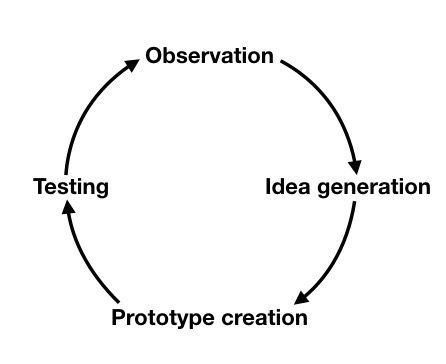
\includegraphics[width=0.5\textwidth]{PrototypeCreation}
\caption{Redogörelse för de fyra stegen för optimal design.}
\end{figure}

Enligt upphovsmannen till UX, Donald Norman [13] består människa-centrerad designprocess av fyra steg som itereras enligt figur 2.1. I boken “The design of everyday things” [14] skriven av samma man tas det upp att denna metod även brukar kallas för “the spiral method” och syftar på att leverera framsteg vid varje iteration. Dessa fyra steg är:  

\begin{enumerate}
\item Observation handlar om att undersöka och förstå problemet. Det handlar om att undersöka och observera slutanvändaren för att kunna förstå deras behov, intresse och motivationer. Det görs genom att observera, lyssna och intervjua användarna. I detta steg bestäms designkraven. Med hjälp av undersökningen kan designern skapa \textit{personas}, vilket är användarprofiler som representerar slutanvändarna och inkluderar information om deras motivationer, mål, behov och förväntningar som beskrivs i boken “Universal Principles of Design” [15]. Dessa användarprofiler skapas i början av ett projekt och kan ändras i ett senare skede vid behov enligt Kim Flahertys artikel “Are Your Personas Outdated? Know When It’s Right To Revise”[16].

\item Idéskapande går ut på att baserat på designkraven hitta lösningar som uppfyller dessa krav. Tillvägagångssättet för den delen av designprocessen görs enligt följande tre steg:
\begin{itemize}
\item att vara kreativ och frambringa många idéer,
\item att undvika att kritisera dessa idéer, att vara kreativ utan hänsyn till begränsningar,
\item att ifrågasätta allting, även det uppenbara. 
\end{itemize}

\item Prototypskapande går ut på att skapa en eller flera prototyper på lösningar som togs fram i idéskapandet. Att experimentera med olika designs, demonstrera användargränssnittet till ledningen och kontrollera om produkten är funktionell och användbar är en del av detta steg. En känd prototypteknik är “Wizard of Oz”. I denna teknik skapas prototyper som efterliknar stora och komplexa system innan de är gjorda. Det ger möjligheten att presentera hur produkten skulle interagera med användaren. 

\item Testning handlar om att observera interaktionen mellan prototypen och användaren. Det kan även göras genom demonstration av olika versioner av användargränssnittet till användarna, intervjua användaren, ställa frågor, använda sig av enkäter för att kunna identifiera svårigheter med användargränssnittet. 
 
\end{enumerate}

I boken “The design of everyday things” [14] diskuteras även att genom iterationen av dessa fyra steg möjliggörs ständigt förbättring av användargränssnittet. När kraven för användargränssnittet är specificerade skapas det en prototyp och den testas för att säkerställa att dessa krav uppfylls. UX-designern får återkoppling från personerna som testar användargränssnittet och resultatet av testningen blir då grunden för en ny iteration som ska påbörjas. Efter varje iteration förbättras användargränssnittet, det blir mer riktat till slutanvändarens krav och produktens kvalité ökas.

\subsection{Utmaningar i UX-designprocessen}

I rapporten “User experience prototyping - a literature review” [17] diskuterar Tuomas Nissinen \textit{fidelity}-aspekten av prototyper som tas fram under designprocessen. \textit{Fidelity} definieras som det koncept som betecknar hur lik en prototyp är slutprodukten. Det finns prototyper som tillämpar olika nivåer av \textit{fidelity} där nivåerna kategoriseras enligt: \textit{low-fidelity} prototyper, \textit{high-fidelity} prototyper, \textit{mixed-fidelity} prototyper och \textit{multi-fidelity} prototyper. Dessa prototyper används vid olika situationer då kostnad, tid och syfte kan variera. \textit{Low-fidelity} kan göras både med papper och penna och på datorn. Den syftar på att presentera ett koncept eller idé istället för att presentera funktionaliteten av hela systemet. Dessa prototyper brukar göras tidigt i designprocessen, är snabba och har extremt låg kostnad. Några nackdelar med dem är att de har begränsningar angående användbarheten och testningen. En \textit{high-fidelity} prototyp har däremot all funktionalitet av systemet samt stödjer användarinteraktion med det. Den är väldigt lik slutprodukten och är väl anpassad för testning. Stödet för interaktiv funktionalitet gör dessa prototyper speciellt användbara vid upptäckt av användbarhetsproblem. Nackdelarna är dock att de är mycket mer tidskrävande än \textit{low-fidelity} prototyper samt att de är mer kostsamma att ta fram. \textit{High-fidelity} prototyper är inte heller anpassade för visualisering av komplex funktionalitet. \textit{Mixed-fidelity} och \textit{multi-fidelity} prototyper är blandningar av de tidigare nämnda prototyperna. Enligt Tuomas Nissinen är skapandet av interaktiva prototyper en stor utmaning för designers. Detta eftersom det skulle vara väldigt tidskrävande att stödja interaktiv funktionalitet i \textit{low-fidelity} prototyper eller implementera komplex funktionalitet i \textit{high-fidelity} prototyper.

Enligt Kate Pernice i Nielsen Norman Group [18] måste en prototyp av ett användargränssnitt testas för att möjliggöra bedömningen av dess användbarhet. Vid testning av prototypen måste alltså användaren få gensvar från prototypen vid handlingar och detta kan göras på två sätt. Det ena sättet går ut på att en person som är bekant med designen ska ge gensvar till användare testar prototypen och en sådan prototyp kallas för statisk. Det andra sättet som implementera dessa gensvar vilket resulterar i en interaktiv prototyp. Skapandet av en sådan prototyp kan bli tidskrävande. Även Pernice lyfter fram de områden där \textit{fidelity} kan variera vilka är interaktivitet, innehåll, kommando och visuellt. 

Vid utveckling av design för ett system, en tjänst eller en produkt krävs det även ett team som ska utveckla det som ligger bakom designen och utgör funktionaliteten. Teamet är delar av större organisationer och enligt en undersökning gjord av Project Management Institute [19] använder sig 71\% av de 3234 organisationer från olika branscher som deltog i undersökningen, av Agila metoder ibland, ofta eller alltid. När UX-designers ska följa Agila metoder kan det bli problematiskt. I en rapport skriven av Michael Budwig, Soojin Jeong och Kuldeep Kelkar vid namn “When User Experience Met Agile: A Case Study” [20] beskrivs svårigheter som kan uppstå vid denna situation. På grund av att UX-teamet behöver utveckla designen innan utvecklingsteamet har utvecklat det bakomliggande systemet skedde det ofta att UX-teamet inte kunde få nödvändiga inputs från utvecklingsgruppens medlemmar. Vid uppkomsten av problem och nya krav för produkten i sprinter är UX-teamet tvungna att hantera både nya problem som har uppkommit, de som var kvar sedan tidigare och samtidigt leverera sina primära projekt i tid. Detta kan orsaka en stressig och negativ arbetsmiljö för UX-teamet. 

I rapporten “Experience Prototyping” [21] påpekas det att designers borde utforska genom att göra, eftersom även små ändringar i ett användargränssnitt kan ha stora konsekvenser i den slutliga användarupplevelsen. Rapporten lyfter även fram betydelsen av skapandet av flera prototyper och påverkan de kan ha på slutprodukten. Detta eftersom en enda prototyp inte är tillräcklig för att designern ska kunna bestämma vilka element som ska användas och hur de ska presenteras i användargränssnittet. Ett sätt att ta reda på designmöjligheter och identifiera möjliga problem är genom direkt användarinteraktion med systemet vilket uppnås med \textit{high-fidelity} prototyper vilket oftast är kostsamt och därför kan det hända att det ofta inte är möjligt att genomföra.

I en undersökning som gjordes med designers av användargränssnitt i rapporten “How is User Interface Prototyping Really Done in Practice? A Survey of User Interface Designers” [22] observerades och analyserades designers som designar användargränssnitt, även kallade UI-designers, vanor vid design av användargränssnitt. 65\% av de deltagande UI-designerna föredrar att använda sig av verktyg som kommer ge \textit{low-fidelity} eftersom det går snabbt att skapa. Av de UI-designers som föredrar att använda sig av \textit{high-fidelity} verktyg är det 85\% som gör det eftersom det modellerar det slutgiltiga systemet korrekt. Enligt undersökningen är den vanligaste metoden för att ta fram ett användargränssnitt att rita. Detta trots att 48\% av UI-designerna anser att slutanvändare inte tar \textit{low-fidelity} prototyper seriöst och 39\% av deltagarna anser att de inte kan testa komplexa interaktioner. En tanke för framtida designverktyg var att de borde ha dessa två aspekter i fokus - snabbhet och korrekthet. 

I rapporten “User Interface Prototyping: Tools and Techniques” [23] presenteras ett antal krav för prototypverktyg vid samling av viktig information för det systemet som ska byggas, sådan information kan vara vilka uppgifter användaren ska kunna utföra vid interaktion med systemet men även användargränssnittets utseende. Kraven som ett prototypverktyg ska ha är att det bland annat ska: 

\begin{itemize}
\item vara enkelt att använda på så sätt att alla medlemmar i ett utvecklingsteam ska kunna delta i utvecklingen av prototypen,
\item  kunna underlätta utförandet små förändringar i användargränssnittet samt kunna se tillämpning av dessa, 
\item ge designers omfattande kontroll av designdetaljer,
\item kunna vara så likt slutprodukten som möjligt och möjliggöra användarinteraktion, 
\item kunna erbjuda versionshantering för prototyper för att ge designern möjligheten att återanvända redan skapade designer.

\end{itemize}

\section{Visualiseringselement} 

I detta avsnitt presenteras sätt som beskriver hur dataströmmar kan visualiseras och utmaningar i visualiseringen. 

\subsection{Visualiseringselement}

För att presentera datamängder finns det en mängd vanligen använda element, såsom linjediagram, stapeldiagram, cirkeldiagram samt punkter eller regioner i färg i kartor. Vid tillämpning av dessa element finns det egenskaper som kan påverka förståelsen av datat. Några av dem är vilket intervall data kommer presenteras i, hur snabbt data kommer uppdateras och hur länge data kommer vara synligt innan det försvinner. Även estetiska egenskaper som färg, storlek och placering är viktigt vid presentation av element.

Enligt rapporten “Visualization of Online Datasets” [24] är stapeldiagram, linjediagram och cirkeldiagram några av de använda diagram som är enklast att förstå och används för visualisering av data. De beskrivs lite mer detaljerade nedan:
\begin{itemize}
\item Stapeldiagram används för visualisering av kategoriska data med diskreta värden.
\item Linjediagram är lämpliga för visualisering av kontinuerliga värden. Värden presenteras som flera punkter som är anslutna med varandra och bygger en linje. Detta diagram har hög läsbarhet.
\item Cirkeldiagram är ett diagram som används mest för presentation av proportionella data. Varje del av cirkeldiagrammet är märkt med en färg och en etikett för att representera en procent av de data som presenteras. Den är mest lämplig för presentation av data som delas upp i högst sex kategorier för att kunna behålla sin effektivitet. 
\end{itemize}	

\subsection{Utmaningar}

Rapporten “Challenges in Visual Data Analysis” [25] presenterar de största utmaningarna inom visuell analys vilket innebär visualisering av stora, heterogena och dynamiska mängder data. Visuell analys innebär att representera data och ge människor möjligheten att interagera med dessa data för att ta beslut och dra slutsatser. I rapporten lyfts det även fram att koncept såsom representation, uppfattning, interaktion och beslutsfattande är avgörande för presentation och analys av data. En av utmaningarna som förekommer i visuell analys är visuell skalbarhet vilket innebär att kunna presentera stora datamängder och fokusera mer på detaljer och enskilda element. En annan stor utmaning som finns i visuell analys är att kunna tolka data på ett korrekt sätt och dra slutsatser. Detta beror väldigt mycket på metoder som används för att processa rådata och kvalité på rådata. Det gäller då att åtgärda möjliga fel på rådata, till exempel dubbletter, och skapa en stabil design för visualiseringen. Analys av tidsberoende dataströmmar är också en utmaning för visuell analys eftersom bra komprimerings- och hanteringsmetoder för data behövs. Det är viktigt att kunna analysera data och presentera värdefulla resultat för att möjliggöra snabb identifiering av till exempel anomalier i data. 

Ytterligare en svårighet med att presentera dataströmmar är att hastigheten som data kommer in kan vara extremt hög enligt rapporten “Visual analysis of dynamic data streams” [26]. Detta kan försvåra arbetet för forskare eller analytiker då data ska analyseras och beslut ska fattas i realtid. Dessutom kan data som passerat vara relevant för aktuella data vid vissa beslutsfattningar. Eftersom dataströmmar ofta innehåller väldigt mycket information kan det vara lämpligt att användare kan filtrera och extrahera den data som är relevant för deras problem och behov. Även att kunna kombinera, sätta ihop och jämföra olika aspekter av data kan öka förståelsen och underlätta analysen för användaren. 

\section{Elastic Stack} 

Elastic stack är ett verktyg som kan ta data från vilken källa som helst, i vilket format som helst, och söka, analysera och visualisera det i realtid. Den består av fyra open-sourceprojekt som är Beats, Logstash, Elasticsearch och Kibana som presenteras mer i detalj nedan. Användning av Elastic stack är gratis men det finns begränsningar i utrymme och vissa extrafunktioner som kan betalas. [27]


\subsection{Logstash} 

Enligt produktbeskrivningen för Logstash på Elastic Stacks hemsida [28] är Logstash en dataprocessor för server-sidan som samlar data från många olika källor samtidigt, förvandlar dem och skickar sedan dem till det \textit{stash} som anges. Detta är ofta Elasticsearch eftersom de har en mycket stark synergi mellan varandra. Processhanteringen är en pipelinemed tre steg: inputs $\rightarrow$ filter $\rightarrow$ outputs. Inputs genererar händelser, filter ändrar dem och outputs skickar dem någon annanstans.

\subsection{Beats}

Enligt Beats produktbeskrivning på Elastic Stacks hemsida [29] är Beats en plattform för lätta och enkla datasändare. De kan skicka data från tusentals maskiner till Logstash eller Elasticsearch. De är installerade på servrar och centraliserar icke modifierade data till Elasticsearch. Om datat behöver bearbetning kan Beats skicka det till Logstash för ändring och analysering av data. Några exempel på olika Beats är Filebeat som används för att samla loggfiler, Metricbeat för att samla mätvärden från dina system och tjänster och Packetbeat för att samla nätverksdata. 

\subsection{Elasticsearch}

Elasticsearch är en JSON-baserad, RESTful sök och analysmotor som lagrar och indexerar data och gör dem tillgängliga för analys och visualisering enligt produktbeskrivningen för Elasticsearch på Elastic Stacks hemsida [30]. Det är Elastic Stacks huvudmotor och möjliggör lagring, sökning och analys av stora datamängder snabbt och i nära realtid vilket innebär att det finns en liten latens från det att ett dokument indexeras tills dess att det blir sökbart. Elasticsearch passar bäst för applikationer som är konstruerade för att hantera nära realtidsdata som behöver bearbetas och analyseras snabbt. 
 

\subsection{Kibana}

Kibana används för att visualisera det som är lagrad i Elasticsearch och är baserat på HTML, JavaScript och Bootstrap enligt Kibanas produktbeskrivning på Elastic Stacks hemsida [31]. Kibana möjliggör en mängd olika visualiseringar av data med vanligen använda UI-element som beskrivs nedan:

\begin{itemize}
\item Diagram: areadiagram, värmekarta, horisontellt och vertikalt stapeldiagram, linjediagram, cirkeldiagram.
\item Data: datatabell, mätare, målmätare, siffror.
\item Kartor: koordinater i karta, regioner i karta.
\item Övriga: titlar, taggmoln, sök.
\end{itemize}

I dessa UI-element aggregeras data automatiskt av Kibana vid val av fält. Det kan vara fält som representerar tid, namn, geografisk koordinat, summa, m.m. För att Kibana ska kunna aggregera dessa egenskaper i data måste de vara kartlagda i Elasticsearch. Kartläggningen går ut på att specificera vilka fält som representerar vad. UI-elementen har anpassningsbara egenskaper som rör visualiseringen av datat, till exempel färg, etiketter på axlar i grafer, det maximala antalet olika värden samt specifika modifieringar för vissa UI-element. När flera UI-element sparats kan de kombineras med varandra för att bilda \textit{dashboards}. Ett UI-element går att använda i flera \textit{dashboards} och om en ändring görs på UI-elementet ändras det på alla ställen. Att ändra och spara är en snabb process som kan göras på ett fåtal knapptryckningar vilket underlättar vid framtagning av en \textit{dashboard} och ändringar som bör göras i den. \textit{Dashboards} går även att bädda in i webbsidor genom HTML vilket kan vara väldigt användbart vid kombination med olika \textit{dashboards}. Ytterligare en aspekt vid framtagning av \textit{dashboards} i Kibana är att det som utvecklas är den faktiska produkten som ska användas av slutanvändaren. Vid interaktion med UI-element i Kibana filtreras data och filtret tillämpas då på alla UI-element i hela \textit{dashboarden}.

Vid skapandet av en interaktiv \textit{dashboard} finns det en mängd egenskaper som går att anpassa. Det går att ställa in en automatisk uppdateringsfrekvens som hämtar nya data på intervall mellan 5 sekunder och 1 dag. Det går även att specificera under vilket datum- och tidsintervall data ska visualiseras. Det kan då vara relaterat till nuvilket är tidpunkten som användaren sitter framför \textit{dashboarden} eller två fixerade tidpunkter. Ett exempel hade kunnat vara att visa all data från en minut sedan till nu och uppdatera datat varje minut

I Kibana finns även utvecklarverktyg som erbjuder kraftfulla sätt att interagera med Elastic Stack. Med den inbyggda konsolen kan utvecklare undvika att skriva kommandon i terminalen och istället utveckla Elasticsearch-data direkt i Kibana. I den betalda versionen av Elastic Stack finns det även möjlighet för tillämpning av maskininlärning på data i Elasticsearch, notiser vid ändringar av specificerade data, rapportgenerering av en eller flera visualiseringar i Kibana.

\afterpage{\null\newpage}
\chapter{Metod}

I detta kapitel presenteras vilka metoder som användes för att uppfylla målen definierade i 1.2.

\section{Litteraturstudie}

För att identifiera utmaningar i den traditionella designprocessen genomfördes en litteraturstudie under förstudien. Detta för att ta reda på vad som skulle stå i fokus under utvärderingen av designprocessen som skulle bli framtagen med Kibana. Under förstudien genomfördes även en litteraturstudie för att ta reda på svårigheter inom visualisering för att kunna välja en typ av data som har visualiseringsutmaningar. Litteraturstudien utfördes genom analyser av relaterade arbeten och rapporter.

\section{Utvärdering av UX-designprocessen vid användning av Kibana}

Efter att produkten tagits fram och UX-designprocessen specificerats gjordes en utvärdering av UX-designprocessen. Denna utvärdering utfördes av UX-designers via ett formulär där hela UX-designprocessen vid användning av Kibana beskrevs. Även en beskrivning av visualiseringsverktyget Kibana inkluderades för att möjliggöra UX-designers som inte haft erfarenhet av verktyget att besvara formuläret. I formuläret skulle sedan påståenden besvaras angående olika aspekter av UX-designprocessen i Kibana såsom begränsningar och särskilda funktioner. Erfarna UX-designers var vana vid att arbeta enligt den traditionella UX-designprocessen och ansågs därför som lämpliga kandidater för undersökningen. Författarna definierade en erfaren UX-designer som en person som hade tre år eller mer erfarenhet av att arbeta med design. Formuläret skickades ut till 60 kandidater genom deras profiler på LinkedIn och formuläret kan hittas i A.1 i Appendix.

Det som utvärderingen fokuserade på var svårigheter inom UX-designprocessen, främst det tredje steget, prototypskapande och det fjärde, testning. Inom skapandet av prototypen fanns det svårigheter vid att få prototypen och slutprodukten att vara lika främst gällande det visuella, innehållet, interaktionen och funktionaliteten eftersom utvecklare och designers använde olika verktyg. Ändringar som skulle göras på designen kunde även komma att bli kostsamma och därför fokuserade även utvärderingen på optimering av ändring av användargränssnittet. Vid testningen var det en del faktorer som försvårade att testa den riktiga funktionaliteten på produkten, bland annat att det var väldigt tidskrävande och att designers inte alltid visste systemets begränsningar. UX-designprocessen utfördes så många omgångar det krävdes för att få kunden nöjd inom tidsramen för projektet. För att utföra testningen genomfördes djupintervjuer i grupper med 5 personer. Deltagarnas användarupplevelse noterades genom ett formulär. Testningen var uppdelad i fyra moment: allmänna frågor, grundläggande trafikförståelse, avancerad trafikförståelse och sammanfattning. De tre första momenten baserades på uppgifter som skulle utföras av deltagarna. Dessa uppgifter betygsattes sedan av deltagarna baserat på svårighet vid utförandet genom en skala från ett till fem eller ett till tio. Frågorna som ställdes och de möjliga svarsalternativen finns i A.3 i Appendix.


\section{Utvärdering av kommunikationen mellan Agila utvecklare och UX-designers}

En utvärdering gjordes även av kommunikationen mellan Agila utvecklare och UX-designers eftersom det har visat sig vara en svårighet. Under projektets gång fick författarna erfarenhet av båda rollerna eftersom de dels skapade systemet och designen till \textit{dashboarden}. Utvärderingen gjordes genom en analys av tankar, erfarenheter och noteringar som gjorts av författarna under projektets gång. 


\section{Förberedelse av data för visualisering}

För att möjliggöra utvärderingen av designprocessen vid användning av Kibana skapades ett användargränssnitt med hjälp av Kibana som skulle visualisera Transportstyrelsens data från betalstationer.

För att kunna presentera data användes Elastic Stack. Anledningen till att just detta verktyg valdes är på grund av övertaget denna produkt har på marknaden. Den är snabb vid sökningar och analyser, gör filtrerings- och modifiering processen smidig och erbjuder ett helt anpassningsbart användargränssnitt. Dessutom är det en väldigt stabil produkt som används av stora företag som bland annat Facebook, eBay, Netflix och Slack enligt Elastic Stacks lista på kunder [32].  

En utmaning i visualisering av strömmande data har varit visuell skalbarhet och beslutsfattande. Ett annat vanligt problem inom visualisering av strömmande data var hastigheten som data skulle komma in och kombination av data vid visualisering för ökande förståelse. Ett mer generellt men ofta förekommande problem vid användning av data är att de inte är i den önskade formen och därför krävs det modifiering för att kunna använda dem på det önskade sättet. Vid skapandet av \textit{dashboarden} skulle de ovannämnda utmaningarna ligga i fokus. I det här projektet skulle visualisering av strömmande data examineras och därför behövdes det en dataström. Data som användes var statisk, icke konsistent och ofullständigt därför valdes den följande implementationen.

I Figur 3.1 representerar pilen dataflödet från det att data hämtas till att de visualiseras. 

\begin{figure}[h]
\centering
\includegraphics[width=1\textwidth]{Systemarkitektur}
\caption{Redogörelse för systemarkitektur.}
\end{figure}

Det började med en RESTful webbtjänst som efterfrågade Transportstyrelsens data genom det öppna API:et som fanns tillgängligt på Transportstyrelsens hemsida. Vid förfrågan av data under en viss tidsperiod returnerades en lista med passager och deras egenskaper. Dessa passager modifierades och skickades vidare till Logstash som skulle skicka data till Elasticsearch. Efter det hämtades data från Elasticsearch in i Kibana för att möjliggöra visualiseringen av dem.  

Eftersom data som användes var statisk skapades en dataström av dessa data med hjälp av webbtjänsten. Detta gjordes genom att modifiera tiden i data som kom in i webbtjänsten, i sekundnivå. För att kunna använda dataströmmen som skapades och visualisera den i Kibana så krävdes modifiering av data. Detta gjordes genom att ändra format på datatyper, som tid och datum, vilket gjordes i webbtjänsten innan data skickades vidare till Logstash. Dessutom var det nödvändigt att lägga till information om geografiska punkter på den data som visualiserades för att möjliggöra visualisering av data i kartor. Eftersom regioner som skulle visualiseras saknades i Kibana behövdes även denna information tas fram. Informationen om regioner, som i detta fall var svenska kommuner och län, som fanns tillgängliga var i ett format som inte var kompatibelt med Kibana. På grund av detta skapades ett dokument som innehöll denna information och lades till i Kibanas regionsdata. Ytterligare ett tillägg som behövdes på data var geografiska koordinater för betalstationer. Detta för att kunna visualisera trafikintensitet baserad på betalstationer. Det gjordes genom att ta fram ett dokument som innehöll koordinater för betalstationerna. Informationen om koordinater lades till i all data som hämtades genom webbtjänsten och skickades vidare till Logstash. 

I tabell 3.1 presenteras vilka egenskaper en passage hade efter modifiering. Dessa egenskaper användes sedan för visualisering. 
\newpage
\captionsetup[table]{name=Tabell}

\begin{table}[h!]
  \begin{center}
    \caption{En passage och dess egenskaper efter modifiering.}
    \label{tab:table1}
    \begin{tabular}{|p{3cm}|p{3cm}|p{3cm}|p{3cm}|}
         \hline
      \textbf{Fält} & \textbf{Format} & \textbf{Exempel} & \textbf{Beskrivning}\\
      \hline
      Datum & YYYY-MM-DD & “February 27th 2015” & Datum för passage\\ % <--
        \hline
      Klockslag & HHMM& “06:56” & Klockslag för passage\\ % <--
        \hline
      SkatteObjekt & Sträng & “GBG”
 & Område för avgift/skatt\\ % <--
        \hline
      Betalstation & Sträng & “Hjalmar Brantingsgatan” & Betalstation\\ % <--
        \hline
      Riktning & Sträng & “Ut” & Körriktning\\ % <--
        \hline
      Län & Sträng & “Västra Götalands Län” & Län\\ % <--
        \hline
      Kommun & Sträng & “Göteborg” & Kommun\\ % <--
        \hline
      Körfältsnummer & Nummer & “4” &  Körfältet som fordonet var i vid passage\\ % <--
        \hline
          Postnr & Sträng & “418xx”
 & Postnr - endast de 3 första siffrorna\\ % <--
        \hline
          Fordonstyp & Sträng & “PERSONBIL” & Fordonstyp\\ % <--
        \hline
          TidStämpel & yyyy-MM-dd'T'HH:mm:ss
 & “February 27th 2015, 07:56:03” & Tidsstämpel för passagen med datum och tid, på sekundnivå 
\\ % <--
        \hline
Geografisk Placering & Sträng & “57.718564, 11.994575” & 
Koordinat för betalstationens 
\\ % <--
        \hline
    \end{tabular}
  \end{center}
\end{table}


\section{Visualisera data i en interaktiv \textit{dashboard} i Kibana}

För att visualisera data i en interaktiv \textit{dashboard} i Kibana skapades först alla UI-element och sedan integrerades de in i en \textit{dashboard}. De UI-element som användes var de som fanns tillgängliga i Kibana och som var passande för syftet. De element som användes var:

\begin{itemize}
\item Taggmoln:
\begin{itemize}
\item Taggmoln med olika områden med betalstationer i Sverige, där störst text visar störst antal
\item Taggmoln med de fem mest populära betalstationerna i det specifika området, där störst text visar störst antal
\end{itemize}
\item Karta med koordinater:
\begin{itemize}
\item Karta med koordinater för alla betalstationer utplacerade i Sverige
\end{itemize}
\item Karta med geografiska områden:
\begin{itemize}
\item Karta med län där fordonsägare bor, där starkast färg är flest antal fordon
\item Karta med kommuner där fordonsägare bor, där starkast färg är flest antal fordon
\end{itemize}
\item Stapeldiagram:
\begin{itemize}
\item Stapeldiagram med de mest trafikerade betalstationerna i det specifika området med fordontypsfördelning
\item Stapeldiagram med trafikintensitet med fordontypsfördelning
\end{itemize}
\item Cirkeldiagram:
\begin{itemize}
\item Cirkeldiagram med fordontypsfördelning
\item Cirkeldiagram med körfältsfördelning
\end{itemize}
\item Antal:
\begin{itemize}
\item Antal fordon den senaste minuten i det valda området
\end{itemize}
\item Sök:
\begin{itemize}
\item Sökning baserat på betalstationer
\end{itemize}
\end{itemize}

Vid specificering av data som skulle ingå i ett UI-element gjordes automatiska aggregeringar av Kibana vid val av fält. Aggregering gjordes på termer i valda fält, koordinater och datum. För termer i valda fält specificerades ett fält och sedan skapades automatiskt aggregeringar baserat på flest/minst antal gånger värdet i detta fält uppkom. Eftersom de UI-elementen som skapades kunde återanvändas på flera olika \textit{dashboards} skapades flera versioner av användargränssnittet vid varje iteration. 


\afterpage{\null\newpage}

\chapter{Resultat}

I det här kapitlet kommer designprocessen vid användning av Kibana samt tillämpningen av den att förklaras. Även en utvärdering av den framtagna designprocessen presenteras i detta kapitel.  

\section{UX-Designprocess vid användning av Kibana}

UX-designprocessen som togs fram under detta projekt följde stegen i figur 4.1. Målet med varje iterering var att förbättra produkten och komma närmare kundens krav. Itereringen upprepades tills dess att kunden accepterade produkten. Observation och idéskapande följde den traditionella designprocessen och beskrivs i kapitel 2.1.5 medan produktskapande och testning fick en ny betydelse.Stegen i UX-Designprocessen vid användning av Kibana beskrivs nedan:

\begin{figure}[h]

\centering
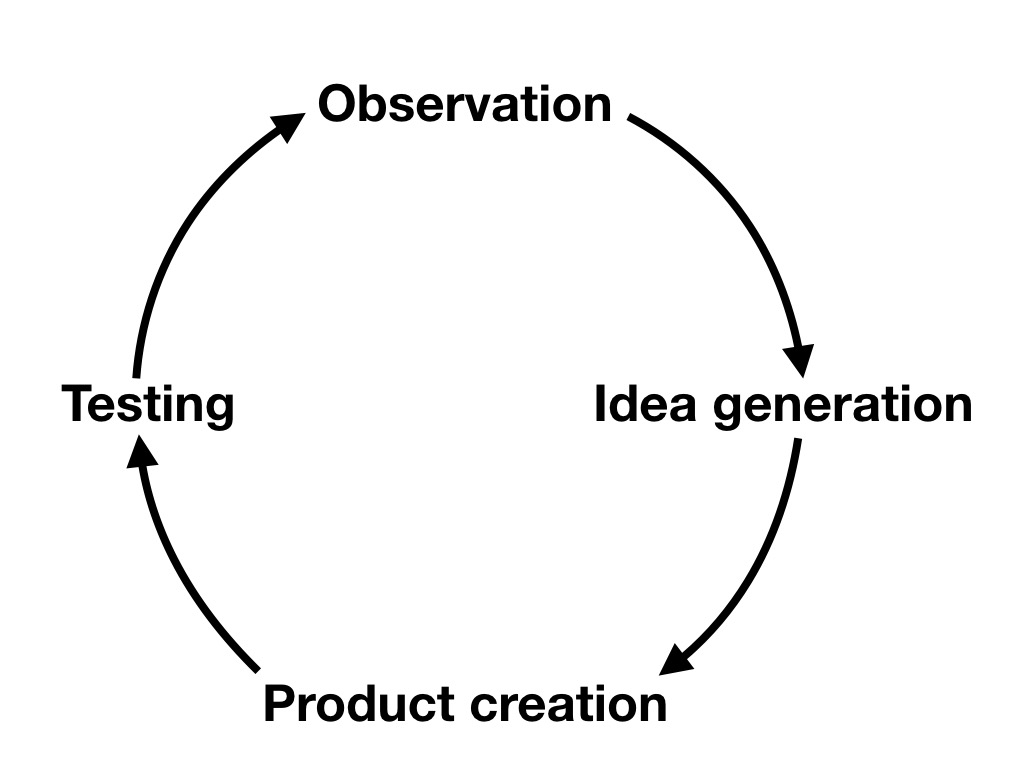
\includegraphics[width=0.5\textwidth]{ProductCreation}
\caption{Redogörelse för de fyra stegen i designprocessen vid användning av Kibana.}
\end{figure}

\begin{itemize}
\item Produktskapande gick ut på att skapa produktens användargränssnitt. Att experimentera med olika designer, demonstrera användargränssnittet till ledningen och att kontrollera om produkten är funktionell och användbar var del av detta steg. \textit{High-fidelity} nåddes på grund av att ingen prototyp togs fram och istället skapades produkten som kunde tillämpa all funktionalitet systemet kunde erbjuda.
\item Testninghandlade om att observera interaktionen mellan produkten och användare. Det kunde även göras genom demonstration av olika versioner av användargränssnittet till användarna, intervjua användaren, ställa frågor, använda sig av enkäter för att kunna identifiera svårigheter med användargränssnittet. Produkten testades mot systemet och all funktionalitet gick att testa mot användargränssnittet. Användarinteraktionen gjordes som om \textit{dashboarden} var slutprodukten. Vid önskemål av testare kunde även UI-element i produkten ändras. 
\end{itemize}

\section{Utvärdering av UX-designprocessen vid användning av Kibana}
Formuläret för utvärdering av UX-designprocessen vid användning av Kibana besvarades av 32 lämpliga kandidater. Eftersom formuläret skickades ut till 60 personer resulterade detta i en svarsfrekvens på 53\%. En sammanfattning av utvärderingen blev följande:

\begin{itemize}
\item Att Kibana möjliggjorde \textit{high-fidelity} vid aspekterna interaktion, funktionalitet och visualisering tyckte 88\% av deltagarna var bra eller mycket bra egenskaper.

\item 69\% av deltagarna stördes väldigt mycket eller stördes lite av att det fanns begränsningar i hur anpassningsbara vissa UI-element var. Som till exempel att tjockleken på staplar i stapeldiagram och tjockleken på cirkeldiagram med centrumhål inte gick att anpassa. 22\% av deltagarna stördes inte alls av denna begränsning.

\item Att fonten inte var så anpassningsbar i UI-element hävdade över 50\% av UX-designerna som svarade på formuläret att det störde dem väldigt mycket.

\item 78\% av deltagarna stördes, väldigt mycket eller lite, av att de inte var helt fria vid placeringen av UI-element på \textit{dashboarden}. 

\item Kibana hade egenskapen att inkludera en \textit{dashboard} i en webbsida där bland annat font, rubriker och fördelning kunde anpassas. 75\% av deltagarna tyckte att denna egenskap var användbar eller mycket användbar.

\item I Kibana kunde uppdateringsfrekvensen av \textit{dashboarden} som minst specificeras till 5 sekunder, vilket kunde ha en påverkan vid visualisering av strömmande data. Detta tyckte 38\% var dåligt och 31\% var skäligt. En kommentar var att det berodde på dataströmmens detaljnivå.

\item Att det var en väldigt intuitiv utvecklingsmiljö i Kibana tyckte 56\% av deltagarna var en väldigt bra egenskap och 38\% tyckte att det var en bra egenskap.

\item För att skapa visualiseringar i Kibana behövde systemet vara fulländat först. 44\% av de tillfrågade UX-designerna tyckte att detta påverkade designprocessen negativt och 9\% tyckte att påverkan var väldigt negativ. Dock tyckte 16\% att det var positivt eller väldigt positivt. Kommentarer till denna fråga var att det var positivt men på grund av att det inte förekommer ofta att systemet är fulländat innan UX-designers ska påbörja sitt arbete tyckte en stor andel att det påverkade negativt.

\item Vid interaktion med UI-element kunde data filtreras. Om filtrering gjordes på ett UI-element tillämpades detta på alla UI-element på hela \textit{dashboarden}. Detta höll alltså all data synkroniserad. Detta tyckte 59\% av deltagarna var positivt eller väldigt positivt.

\item Efter att ett UI-element skapats kunde det återanvändas på önskat antal \textit{dashboards} och om UI-elementet skulle modifieras i en \textit{dashboard} hade det ändrats på alla ställen det förekom. Detta tyckte 96\% var positivt eller väldigt positivt.

\item Övriga kommentarer från utvärderingen som var relaterade till UX-designprocessen var att det ofta är väldigt högt prioriterat att vara effektiv i utförandet av designprocessen men det finns undantag då designkraven måste nå en viss nivå och då, för att inte produkten ska bli oanvändbar, prioriteras den effektiva designprocessen bort. Det fanns även en deltagare som tyckte att detta visualiseringsverktyg verkade mer passande för utvecklare som snabbt ville visualisera data. Detta på grund av att det fanns alldeles för mycket begränsningar för UX-designers.
\end{itemize}

\section{Utvärdering av kommunikationen mellan Agila utvecklare och UX-designers}

Svårigheter vid kommunikationen mellan Agila utvecklare och UX-designers eliminerades under UX-designprocessen vid användning av Kibana. Detta eftersom systemet behövde vara fullständigt innan visualiseringar kunde skapas. Eftersom begränsningar inom UX-designen vid användning av Kibana berodde på vilken typ av data som fanns tillgänglig, till exempel om inte geografisk placering fanns tillgänglig gick det inte att visualisera data i en karta. Detta innebar att UX-designers inte behövde kommunicera med utvecklare under UX-designprocessen för att bli informerade om systemets begränsningar. 

\section{Tillämpning av UX-designprocess vid användning av Kibana}

Nedanstående steg upprepades tre gånger och slutprodukten finns tillgänglig i A.5 i Appendix.  

\subsection{ Utforska slutanvändare och ta fram deras behov och krav
}
Det första steget gick ut på att förstå användarna och deras behov. Det gjordes genom att analysera data som skulle presenteras för att komma fram till intressant information som skulle kunna lyftas fram med presentation av data. För att göra detta skapades användarprofiler, även kallas för \textit{personas}, som representerade slutanvändaren av produkten. I dessa \textit{personas} beskrevs användares behov, mål och egenskaper och finns i A.2 i Appendix. \textit{Personas} skapades endast under den första iterationen. Utifrån dessa \textit{personas} definierades designkraven för \textit{dashboarden} gällande visualiseringen av data. De definierade designkraven gick ut på att presentera följande information på \textit{dashboarden}:

\begin{itemize}
\item Hur många bilar åker igenom varje betalstation och/eller stad?
\item Varifrån kommer bilar som åker genom betalstationerna? 
\item Hur många fordon som passerade den senaste minuten? 
\item Hur ser trafikfördelningen ut baserad på riktning? 
\item Hur ser trafikfördelningen ut baserad på körfält? 
\item Vilken är den mest populära fordonstypen?
\end{itemize}

Vid start av varje iteration analyserades resultatet av testningsfasen. 

\subsection{Ta fram lösningar som uppfyller dessa behov och krav }
Detta gick ut på att utforska data som skulle presenteras. Det inspekterades vilka värden som fanns tillgängliga och vilka möjligheter som fanns för att kombinera data för visualisering. Lösningarna blev dessa:
 
\begin{itemize}
\item Trafikintensitet baserat på betalstationer
\item Trafikintensitet baserat på stad
\item Kommun där fordonsägare bor
\item Län där fordonsägare bor
\item Trafikintensitet baserat på fordonstyp 
\item Trafikintensitet baserat på fordonstyp för de mest populära betalstationerna
\item Möjligheten att söka efter en betalstation
\item Riktningsfördelning
\item Körfältsfördelning
\item Antal fordon
\end{itemize}

Efter detta togs förslag om hur användargränssnittet skulle se ut fram. Det ritades ett första utkast för användargränssnittet och visades till en av slutanvändarna för att diskutera möjliga förändringar eller tillägg. 

\subsection{ Implementera lösningarna i en interaktiv \textit{dashboard} i Kibana }
Efter att användare godkände ritningen skapades en \textit{dashboard} i Kibana baserat på den. Vid specificering av data som skulle ingå i ett UI-element gjordes automatiska aggregeringar av Kibana vid val av fält. Aggregering gjordes på värden i valda fält, koordinater och datum. För att aggregera på värden i valda fält specificerades fältet i UI-elementet och sedan skapades automatiskt aggregeringar baserat på flest/minst antal gånger värdet i detta fält uppkom. Under skapandet av \textit{dashboarden} togs flera olika designer fram. Det togs även hänsyn till UX riktlinjer, tidigare teorier inom UI och UX samt användares behov och önskemål. Vid varje iteration skapades nya \textit{dashboards} som tillämpade ändringar baserat på analysen av testresultatet.

\subsection{ Testa produkten mot slutanvändare genom djupintervjuer 
}
Därefter utfördes testning av \textit{dashboarden} i en grupp av fem personer som representerade möjliga slutanvändare. Testningen genomfördes genom att ställa frågor till användaren angående \textit{dashboarden} och att låta användaren utföra specificerade uppgifter på \textit{dashboarden}. Det utfördes tre iterationer av UX-designprocessen vid användning av Kibana. Användaren observerades vid testningen av produkten och handlingar, tankar och åsikter under utförandet noterades och stod i fokus vid förbättring av \textit{dashboarden}. Frågor som ställdes till användarna vid testning och svaren kan hittas i A.3 i Appendix. Svar från dessa frågor och anteckningar från testning användes vid framtagandet av nästa \textit{dashboard}. Vid varje iteration testades varje ny \textit{dashboard} och ett detaljerat testresultat kan hittas i A.4 i Appendix. En sammanställning av testresultatet presenteras nedan. 

\begin{enumerate}
\item Första iterationens testresultat:
\begin{itemize}
\item Allmänna frågor: Vid den första testningen av \textit{dashboarden} tyckte majoriteten av testarna att det var svårt att identifiera varje UI-elements rubrik och de önskade att de skulle sticka ut mer. \textit{Dashboarden} gav ett rörigt och förvirrande intryck. 

\item Grundläggande trafikförståelse: Kartorna var svåra att använda för att filtrera, söka och ta fram information om trafik. Dessutom tyckte testarna att det var svårt och komplicerat att identifiera skillnader på fordonsriktningen och hitta specificerad information i \textit{dashboarden}. Placeringen av element skulle kunna vara mer eftertänkt för att följa en röd tråd och många UI-element visualiserade samma information på olika sätt vilket skulle kunna undvikas. Det fanns en förvirring gällande relationerna mellan UI-elementen. 

\item Avancerad trafikförståelse: Efter de första uppgifterna upplevdes det lättare att hantera \textit{dashboarden} men det förblev svårt att kombinera flera olika UI-element för att ta fram önskad information. Det var otydligt hur interaktion med UI-element i \textit{dashboarden} kunde användas för framtagandet av information. 

\item Sammanfattning: Det uppmärksammades att även mer förklaring gällande UI-element och deras användning borde läggas till. Det önskades också en bättre fördelning av UI-element i \textit{dashboarden} för att öka förståelse och minska förvirringen.
\end{itemize}

\item Andra iterationens testresultat:

\begin{itemize}
\item Allmänna frågor: Den andra testningen visade beskrivningarna och rubrikerna av UI-element hade blivit lättare att identifiera och förstå men det fanns rum för förbättring. Det fanns ett tydligare sammanhang i \textit{dashboarden} men några ändringar skulle kunna göras gällande antalet element som var placerade i \textit{dashboarden}.

\item Grundläggande trafikförståelse: Sökningen underlättades och det var mer lättförståeligt hur önskad information kunde tas fram men det var fortfarande svårt att förstå visa UI-element. Det var dock svårt att identifiera för vilken tidpunkt data representerades.

\item Avancerad trafikförståelse: Det var många UI-element placerade i slutet av \textit{dashboarden} vilket orsakade förvirring och extra letande för att hitta vilket UI-element som skulle användas för framtagandet av önskad information. Uppgifterna utfördes enklare och \textit{dashboard} tillbringade mer förståelse. Det uttrycktes önskemål om mer detaljerad information om betalstationerna utan att behöva interagera med \textit{dashboarden} mer.

\item Sammanfattning: \textit{Dashboarden} var strukturerad och följde ett mönster men det var fortfarande överväldigande i den nedre delen på grund av att det fanns för många UI-element. Dessa skulle kunna sammanfogas så att all data i skulle kunna visualiseras i ett enda element.
\end{itemize}

\item Tredje iterationens testresultat: 

\begin{itemize}
\item Allmänna frågor: Vid den tredje testningen upplevdes \textit{dashboarden} lättare att förstå enligt testarna. Beskrivningen och instruktioner gav tillräckligt med information för att öka förståelsen av data som presenterades i UI-elementen. Detta underlättade även sökningar i \textit{dashboarden}. 

\item Grundläggande trafikförståelse: Sökningen, filtrering och interaktion med UI-element upplevdes lättare. Tidpunkten för data som visualiserades i varje UI-element kunde identifieras tack vare förklaringar i rubriker. Dessutom var relationerna mellan UI-elementen i \textit{dashboarden} lättare att förstå.

\item Avancerad trafikförståelse: Testarna upplevde att uppgifterna kunde utföras mycket snabbare och information togs ut på genom en mer intuitiv process. UI-elementen som användes ledde till en snabbare identifiering av information i \textit{dashboarden} i denna iteration. 

\item Sammanfattning: I sin helhet var \textit{dashboarden} mer intuitiv. Förståelsen av \textit{dashboarden} ökades och det fanns en röd tråd i placering och presentation av UI-element samt i information som visualiserades. 
\end{itemize}
\end{enumerate}

\subsection{Sammanställning av designprocessens genomförande}
I tabell 4.1 finns designprocessens genomförande sammanställd. Designkraven kom från de tänkta slutanvändarna som togs fram under det första steget i UX-designprocessen. Lösningarna togs fram under det andra steget och var konkreta lösningar på designkraven. Visualiseringarna togs fram under det tredje steget och fälten i tabellen var de som användes från en passage för att möjliggöra motsvarande visualisering.

\begin{table}[h!]
  \begin{center}
  \caption{Sammanställning av UX-designprocessens genomförande.}
    \label{tab:table1}
 \begin{tabular}{|p{3cm}|p{3cm}|p{3cm}|p{3cm}|}
      \hline
     \textbf{Designkrav} & \textbf{Lösningar} & \textbf{Visualisering} & \textbf{Fält}\\
     \hline
  \multirow{3}{3cm}{Hur många bilar åker igenom varje betalstation och/ eller stad?} &  Trafikintensitet baserad på stad & Taggmoln  & SkatteObjekt\\\cline{2-4}
  & \multirow{2}{3cm}{Trafikintensitet baserad på betalstationer} & Karta med koordinater
& Geografisk Placering\\\cline{3-4}  
  & &  Taggmoln
& Betalstationer \\ \hline


  \multirow{2}{3cm}{Varifrån kommer bilar som åker genom betalstationerna?} &  Kommun där fordonsägare bor & Karta med geografiska områden  & Kommun\\\cline{2-4}
  &Län där fordonsägare bor
 & Karta med geografiska områden  & Län\\ \hline
 
Hur många fordon som passerade den senaste minuten? &Antal fordon
 & Antal  & PassageObjekt\\ \hline
 
 \multirow{2}{3cm}{Hur ser trafikfördelningen ut baserad på riktning?} &  Riktnings-fördelning&Cirkeldiagram& Riktning\\\cline{2-4}
  &Körfälts-fördelning 
 & Cirkeldiagram  & Körfält\\ \hline
 
 \multirow{2}{3cm}{Vilken är den mest populära fordonstypen?} &  Trafikintensitet baserad på fordonstyp & Cirkeldiagram& Fordonstyp\\\cline{2-4}
  &Trafikintensitet baserad på fordonstyp för de mest populära betalstationerna 
 & Stapeldiagram  & TidsStämpel, Betalstation, Fordonstyp\\ \hline

\end{tabular}
\end{center}
\end{table}

\afterpage{\null\newpage}

\chapter{Analys och diskussion}
I detta kapitel kommer UX-designprocessen vid användning av Kibana analyseras och diskuteras jämfört med den traditionella UX-designprocessen. Även en analys av utvärderingen som gjordes av erfarna UX-designers för den framtagna designprocessen kommer utföras i detta kapitel. 

\section{ Jämförelse mellan UX-designprocess vid användning av Kibana och den traditionella UX-designprocessen}
Den UX-designprocessen som togs fram vid användning av Kibana följde den traditionella UX-designprocessen och var lik den gällande de två första stegen: observation och idéskapandet. Under dessa steg genomfördes arbetet i det här projektet som om de hade genomförts vid tillämpningen av den traditionella UX-designprocessen. De två sista stegen i den framtagna UX-designprocessen som var produktskapandet och testning skiljde sig från de två sista stegen i den traditionella UX-designprocessen som var prototypskapandet och testning. De skiljde sig åt vad det gällde tillvägagångssätt och innehåll. 

Produktskapandet skulle gå till genom att implementera lösningar för det som togs fram under idéskapandet genom att ta fram \textit{dashboards} som hade \textit{high-fidelity}. Detta betydde att varje \textit{dashboard} som togs fram skulle stödja all funktionalitet som systemet erbjöd och skulle kunna vara slutprodukten. Detta var något som var kostsamt vid den traditionella UX-designprocessen eftersom en \textit{high-fidelity} prototyp skulle kräva mycket förberedelse för att kunna efterlikna slutproduktens funktionalitet. 

Under produktskapandet skulle det vara möjligt att återanvända UI-elements som har skapats i flera \textit{dashboards}. På grund av detta effektiviserades skapandet av \textit{dashboards} och flera \textit{dashboards} kunde skapas vid en iteration. Det märkvärdiga med detta var att om ett UI-element användes i olika \textit{dashboards} och det ändrades på ett ställe så skulle det ändras i alla andra \textit{dashboards} som det fanns. En sådan ändring skulle spara tid för UX-designern. 

Testningen i UX-designprocessen vid användning av Kibana hade också några skillnader jämfört med testningen i den traditionella UX-designprocessen. Under testningen skulle resultatet av det föregående steget testas mot möjliga slutanvändare. Skillnaden i testning i de två olika UX-designprocesserna var att i den traditionella UX-designprocessen testades användare mot en prototyp medans i UX-designprocessen vid användning av Kibana testades användare mot en produkt som hade full funktionalitet. Eftersom användare testades på en produkt blev feedbacken mer relevant och möjliggjorde därför högre kvalité av produkten. Dessutom kunde även klagomål och önskade ändringar från användaren åtgärdas direkt vid testning vilket levererade ett bättre resultat.

En stor begränsning som UX-designprocessen vid användning av Kibana hade var att den enbart skulle kunna användas för visualisering av data. Detta var en väldigt stor begränsning jämfört med den traditionella UX-designprocessen som skulle kunna användas på alla olika områden. 

\section{Utvärdering av UX-designprocessen vid användning av Kibana}
Efter utvärderingen av UX-designprocessen kunde det konstateras att majoriteten av deltagarna hade ett positivt intryck av att ta fram och testa en produkt istället för prototyp i UX-designprocessen. Detta eftersom det säkerställde \textit{high-fidelity} av \textit{dashboarden} i tre aspekter: interaktivitet, funktionalitet och visualisering utan att det blev kostsamt eller tidskrävande. Det var även positivt eftersom all funktionalitet i systemet kunde testas på ett ekonomiskt sätt gällande både tid och pengar. 

Däremot var det en väldigt stor del av deltagarna som tyckte att begränsningarna vid visualisering i Kibana var negativt eftersom UX-designerna inte hade den friheten de ofta behövde. Detta inkluderade följande: 
\begin{itemize}
\item att UI-element var inte helt ändringsbara, t. ex. tjockleken på staplarna i ett stapeldiagram
\item att texten i rubrikerna av varje UI-element kunde inte redigeras med avseende på stil, font och storlek
\item att fördelningen av UI-element mest var styrt av Kibana eftersom Kibana försökte fylla hela \textit{dashboarden} med element utan att lämna luckor. 
\end{itemize}

Dessa tre begränsningar kunde vara viktiga i UX-designprocessen eftersom de styrde utseendet av användargränssnittet och därmed även användarupplevelsen. På grund av dessa begränsningar kunde slutsatsen att Kibana försämrade produktens helhetsintryck dras. Om det dock fanns stöd för dessa begränsningar hade Kibana varit ett bättre verktyg för UX-designers eftersom de hade fått den friheten de behövt vid visualiseringen. Ytterligare något som deltagarna tyckte var en positiv egenskap i Kibana var möjligheten att inkludera en \textit{dashboard} i en webbsida med hjälp av HTML. Detta var något som skulle kunna lösa problemen med Kibanas begränsningar. Eftersom Kibana var ett open-sourceprojektsom ständigt utvecklades fanns den potential och en stor möjlighet för mer utveckling och förbättringar.

Deltagarnas åsikter angående uppdateringsfrekvensen som Kibana erbjöd var splittrade. Den högsta uppdateringsfrekvensen som fanns tillgänglig i Kibana var fem sekunder. Detta kunde betraktas som en dålig egenskap eftersom strömmande data med en uppdateringsfrekvens på varje millisekund inte skulle kunna visualiseras så fort nya data fanns tillgänglig. Detta problem hade kunnat bli åtgärdat om Kibana skapade en egenskap som automatiskt justerade uppdateringsfrekvensen baserat på hastigheten som data strömmar in. Däremot hade detta inte varit ett problem alls om dataströmmen har fem sekunder som uppdateringsfrekvens eller lägre och därför skulle det rekommenderas att välja en sådan dataström vid användning av Kibana. 

Deltagarna i utvärderingen betraktade det som väldigt positivt att Kibana hade en intuitiv utvecklingsmiljö och att det var lätt för andra UX-designers eller utvecklare att förstå hur verktyget skulle användas. Detta var en speciellt bra egenskap eftersom arbetsprocessen i projekt effektiviserades om verktygen som användes var lätta att sätta sig in i och använda sig av. 

Majoriteten av deltagarna enades om att Kibanas begränsning angående att systemet behövde vara fulländat innan visualiseringen kunde påbörjas hade en negativ påverkan på UX-designprocessen. Detta eftersom det sällan förekom att systemet kunde bli helt avklarat innan UX-designprocessen påbörjades på grund av ekonomiska skäl och tidsbrist. Detta eftersom det skulle behövas dubbelt så lång tid för ett projekt där systemutvecklare skulle utveckla systemet först och UX-designers sedan designa produkten, jämfört med om dessa två steg hade gjorts parallellt. Om det skulle vara möjligt att dela upp de två stegen så att systemet utvecklades först och produkten designades efter skulle kunna vara något som eliminerade kommunikationen mellan UX-designers och utvecklare. Detta hade därför kunnat göra UX-designprocessen snabbare och mer effektiv men det hade varit svårt att uppnå i många projekt.

I Kibana filtrerades all data i alla UI-element vid filtrering av data. Detta upplevdes som positivt av deltagarna eftersom det kunde underlätta en väldigt tidskrävande process. Ett exempel på hur det hade varit utan denna funktion hade varit då en användare skulle tolka svensk trafikinformation i en \textit{dashboard} i Kibana med 15 UI-element. Om denna användare hade velat göra en filtrering för att bara visa trafik från Göteborg eller baserat på en viss fordonstyp hade denna användare behövt gå igenom alla 15 UI-element och specificera den önskade filtreringen. Detta hade varit tidskrävande och väldigt negativt ur ett UX-perspektiv. Med funktionen i Kibana hade det dock bara varit att göra filtreringen i ett UI-element och då hade allt i \textit{dashboarden} filtrerats. 

Ytterligare en av Kibanas egenskaper som deltagarna tyckte var positiv var möjligheten att återanvända UI-element. Detta skulle kunna spara tid för en UX-designer vid skapandet av flera \textit{dashboards} eftersom de skulle kunna återanvända samma element. Om ett UI-element ändrades på ett ställe skulle det ändras på alla ställen det förekom.

Eftersom denna utvärdering utfördes med 32 deltagare kunde inte resultatet av utvärderingen generaliseras för alla UX-designers. Resultatet var enbart en sammanfattning av en grupp av UX-designers åsikter och tankar baserat på deras arbetserfarenhet inom design. Alla tillfrågade deltagare var opartiska och hade inte hade någon koppling med Kibana sedan tidigare kunde vilket försäkrade en objektiv uppfattning av Kibana. Dock hade det kunnat vara fördelaktigt om deltagarna i undersökningen hade fått testa på Kibana för att kunna få en högre förståelse av begränsningar inom verktyget. Däremot fanns det inte tid för detta på grund av projektets tidsbegränsningar. 

\section{Utvärdering av kommunikationen mellan Agila utvecklare och UX-designers}
Ett problem som togs upp i det här projektet var svårigheterna i kommunikationen mellan Agila utvecklare och UX-designers. Efter framtagandet av UX-designprocessen upplevde författarna att kommunikationen mellan utvecklare och UX-designers eliminerades eftersom det var ett krav att systemet skulle vara klart innan UX-designen påbörjades. Därmed försvann även problemen vid kommunikationen mellan de två parterna. 

Däremot kunde det finnas ekonomiska aspekter i projekt som begränsade både tid och arbetskraft. Dessa begränsningar kunde vara faktorer som orsakade att utvecklare och UX-designers behövde arbeta parallellt från start. Eftersom detta skulle leda till att hela systemet inte kunde var klart innan UX-designen påbörjades skulle inte UX-designprocessen vid användning av Kibana kunna tillämpas. Ett undantag då det skulle gå att tillämpa denna designprocess trots ekonomiska begränsningar skulle vara om data som skulle visualiseras var kompatibel med Kibana och innehöll all information som krävdes för önskade visualiseringar. Då hade utvecklarna inte behövt spendera tid på att modifiera data och därför hade processen för att hämta och visualisera data genom Elastic Stack gått snabbare.

\section{Tillämpning av UX-designprocess vid användning av Kibana} 
I detta avsnitt kommer tillämpningen av UX-designprocessen analyseras. Även för- och nackdelar kommer tas upp och alternativa metoder som hade kunnat ge bättre resultat kommer diskuteras.  Reflektioner som kommer tas upp i detta avsnitt är baserade på författarnas erfarenheter under projektets gång.

\subsection{Utforska slutanvändare och ta fram deras behov och krav} 
Vid framtagandet av \textit{personas} var en av nackdelarna att det inte fanns en tänkt slutanvändare eftersom produkten endast skulle tas fram i syfte att testa UX-designprocessen vid användning av Kibana. Eftersom det inte fanns några tänkta användare togs dessa \textit{personas} fram av författarna och blev då inte så specificerade som de hade kunnat blivit. Det som hade kunnat göras istället var att ställa frågor utåt genom formulär för att ta reda på vad människor hade velat ha som designkrav, eftersom den tänkta målgruppen ändå var en genomsnittlig svensk som var intresserad av trafikinformation i Sverige. Detta hade underlättat vid de andra stegen i designprocessen då det hade funnits ett mer specificerat mål och krav i alla steg.

\subsection{Ta fram lösningar som uppfyller dessa behov och krav}
För att ta fram lösningar krävdes det en hel del förarbete inom Kibana av författarna, som inte hade någon erfarenhet av visualiseringsverktyget. För att ta reda på vilka möjligheter som fanns för visualisering behövde författarna vetskap angående vilka UI-element som fanns tillgängliga, hur de kunde anpassas och hur de kunde kombineras i Kibana. Om personen som skulle använda sig av Kibana hade varit erfaren av visualiseringsverktyget, som författarna upplevde sig vara efter projektet, hade detta dock inte varit ett problem. Därmed hade detta endast varit problematiskt vid den första användningen av Kibana.

\subsection{Implementera lösningarna i en interaktiv \textit{dashboard} i Kibana}

Vid skapandet av UI-elementen upplevde författarna väldigt mycket stöd från Kibana gällande val av data som skulle ingå i dem. Det krävdes endast förståelse kring hur data aggregerades inom Kibana och ett par och efter det valdes fälten som sammanställdes och visualiserades. 

Vad det gällde modifieringen av UI-elementens utseende och deras fördelning i \textit{dashboarden} var det en större utmaning i Kibana. Några av dessa var:

\begin{itemize}
\item Icke modifierbara egenskaper i UI-element.I Kibana var en stor begränsning, ur UX-perspektiv, att det fanns många egenskaper i UI-element som inte gick att modifiera. Till exempel kunde inte tjockleken på staplar i stapeldiagram eller tjocklek på cirkeln i cirkeldiagram med centrumhål ändras. Dessutom fanns det endast 56 färger enligt en viss skala som Kibana erbjöd att välja bland för färger på värden i UI-element.

\item Begränsad modifiering av font. Vid visualisering av data var det väldigt viktigt att kunna beskriva innehållet i varje UI-element med hjälp av rubriker och titlar för att underlätta förståelsen för användarna. Dock var modifieringen av dessa rubrikers egenskaper begränsade. Några av egenskaperna var font, storlek, färg och stil (kursiv, fetstil o.s.v.). I UI-elementen gick det inte att modifiera någonting gällande rubrikens egenskaper. I \textit{dashboarden} kunde det dock skapas ett specifikt UI-element som enbart hade text och i det elementet kunde storlek ändras, dock endast på all text i UI-elementet och inte bara en del av texten, och text kunde få fetstil.

\item Fördelning av UI-element i \textit{dashboarden}. Då UI-elementen skulle sättas ihop i \textit{dashboarden} fanns det en del begränsningar i Kibana. Det var möjligt att placera UI-element i den önskade ordningen men storleken på elementen var inte helt anpassningsbar eftersom det fanns en funktion i Kibana som gjorde att UI-elementen skulle fördelas på \textit{dashboarden} utan några mellanrum eller luckor. En fördel med denna funktion var att även om UI-elementen endast placerades ut på \textit{dashboarden} skapade Kibana en fördelning utan luckor där allt var kombinerat med varandra bra. Dock var det en nackdel då fördelningen behövde specifik modifiering och anpassning eftersom det inte var möjligt. 
\end{itemize}

Dessa ovanstående begränsningar hade en stor påverkan på användargränssnittet och på användarupplevelsen för slutprodukten eftersom det blev svårt att anpassa dessa för att passa slutanvändarens krav. Någonting som hade kunnat förminska eller eliminera dessa begränsningar var möjligheten som fanns i Kibana var att inkludera en \textit{dashboard} i en webbsida genom HTML. Eftersom webbsidan hade varit helt anpassningsbar med avseende på faktorer som font och fördelning av UI-element så hade \textit{dashboarden} kunnat bli förbättrad i sin helhet. Dessutom hade vissa krav som, utan inkludering i en webbsida, hade varit omöjliga att nå kunnat bli blivit möjliga vilket hade resulterat i en nöjdare slutanvändare. På grund av detta projektets tidsbegränsningar fanns det inte tillräckligt med tid för att skapa denna webbsida med inkludering av \textit{dashboarden}.  

\subsection{Testa produkten mot slutanvändare genom djupintervjuer } 
Testningen av produkten genomfördes genom att anteckna och fråga de möjliga slutanvändarna vid djupintervjuer. Eftersom ett stort fokus vid testningen låg vid att de som testades skulle utföra uppgifter som specificerats så ställdes frågor angående svårighetsgraden på uppgiften. De blev ombedda att betygsätta svårighetsnivån. Detta användes sedan för att analysera en iterering och se om förändringar som gjorts i designen hade underlättat för testarna att slutföra en specificerad uppgift. 

Eftersom \textit{dashboarden} upplevdes rörig och ostrukturerad vid första itereringen lades mer beskrivande text för UI-element och distribuering av UI-element i \textit{dashboarden} ändrades. Svårigheterna var att hitta, läsa och tolka texten för att interagera med dem UI-elementen. Kartorna var inte intuitiva och de var svåra att hantera vilket innebar att filtreringen i \textit{dashboarden} var svår att utföra. Därför lades taggmoln till som underlättade filtreringen och hanteringen av \textit{dashboarden}. Det förekom att färgerna i UI-elementen var liknande nyanser vilket försvårade avläsningen av data och därför ändrades de till färgerna som kunde separeras från varandra vilket underlättade avläsning av värden.

Trots alla förbättringar som gjordes efter första iterationen upplevdes \textit{dashboarden} som överväldigande eftersom många UI-element var placerade i den nedre delen av \textit{dashboarden}. Detta löstes genom att sammanställa information som presenterades i ett större UI-element. Ett exempel var att istället för att det fanns fyra olika diagram med olika fordonstyper så organiserades alla den information som presenterades i dem i ett stapeldiagram. Den presenterade antalet fordon i en tidsaxel som kunde filtreras genom ett cirkeldiagram som presenterade fördelningen av alla fordonstyper. Detta resulterade till en bättre förståelse och hantering av \textit{dashboarden}. För att underlätta framtagandet av önskad information ännu mer lades ett sökningsfält till som användes för sökningar baserat på betalstationer. Vid sökning efter en viss betalstation anpassades alla UI-element i denna sökningen. Ytterligare något som gjordes i denna iterering var att den beskrivande texten i UI-elementen förbättrades för att tydligare specificera tidpunkterna för data som presenterades. 

Vid den tredje itereringen upplevdes \textit{dashboarden} mer intuitiv, strukturerad och lättare att interagera med. Information som UI-elementen presenterade var tydlig och beskrivande texten var mer synlig. 

Efter att projektet slutförts ansåg författarna att en bättre metod hade kunnat väljas för att mäta svårighetsnivå på uppgifter. När testarna själva skulle betygsätta svårighet var det väldigt beroende av känslor och åsikter, vilket ur ett UX-perspektiv var bra, men någonting som hade kunnat ge mer konkreta resultat som hade varit värdefullt vid analysen av testningen hade varit att ta tid på en testare från att uppgiften blivit förklarad till att den blivit slutförd. 

\section{Förberedelse av data för visualisering}
För att möjliggöra tillämpningen av UX-designprocessen vid användning av Kibana implementerades \textit{full-stack} utveckling under detta projekt. Vid utvecklingen förekom några svårigheter angående förberedelsen av data inför visualisering. Datakällan som valdes var statisk och mycket tid ägnades åt att simulera en dataström från den källan. Hade författarna istället valt en datakälla som redan var strömmande hade den tiden kunnat läggas på andra saker i projektet. Datakällan som valdes borde också varit så konsistent och fullständigt för visualisering som möjligt. 

I det här projektet lades en stor del av tiden åt modifiering av data så att de skulle gå från en icke kompatibel form i Kibana till att de blev kompatibla med Kibana. Några av modifieringarna som gjordes var att sammanställa datum och tidpunkten av varje objekt i ett nytt fält för att skapa en tidsstämpel som skulle kunna användas senare av Kibana vid visualisering. 

Ytterligare en svårighet som författarna stött på var vid visualisering av geografiska data i Kibana. Datakällan innehöll geografisk relaterad information men inte koordinater för att möjliggöra visualisering i Kibana. Det krävdes en stor informationssökning för att få fram koordinater för den data och mycket tid för modifiering av den informationen för att vara i ett kompatibelt format med Kibana. När informationen hittades i det önskade formatet lades denna information till i varje objekt som hämtades från datakällan. Hela denna process hade kunnat undvikas om det hade valts en datakälla som innehöll all information för visualisering och om informationen var kompatibel med Kibana.

Kibana erbjöd stöd för visualisering av data på kartor men endast för ett begränsat antal länder och eftersom den datakälla som användes i detta projekt innehöll svensk geografisk information som inte fanns tillgängligt ledde detta till en till svårighet. Författarna behövde hitta denna information, modifiera den till rätt format och lägga till den i Kibana för att möjliggöra visualisering av data på kartor. Detta var en tidskrävande process som borde tas hänsyn till när det önskas att utföra visualisering av data i kartor. Kibana är ett open-sourceprojekt och därför finns det många möjligheter för förbättringar av detta.  

\section{Ekonomiska och arbetsmiljömässiga aspekter}
Under detta alla moment i detta projekt har ekonomiska och arbetsmiljömässiga aspekter betraktats. Fokus låg under hela projektet på att se om och hur Kibana kunde underlätta för UX-designprocessen vid visualisering av data. Om Kibana användes med data som var kompatibel med Kibana och systemet var avklarat innan UX-designprocessen påbörjades kunde det påverka de ekonomiska och arbetsmiljömässiga aspekterna positivt. Ur det ekonomiska perspektivet skulle företaget som tillämpade denna UX-designprocess gynnas eftersom mindre tid skulle läggas av arbetarna jämfört med den traditionella UX-designprocessen, vilket skulle spara företaget pengar. Ur det arbetsmiljömässiga perspektivet kunde kommunikationssvårigheter mellan UX-designers och utvecklare elimineras vilket ledde till en bättre arbetsmiljö för båda parterna som kunde lägga fokus på respektive individuella områden.

\afterpage{\null\newpage}

\chapter{Slutsatser}
Det finns många utmaningar och brister inom den traditionella designprocessen för UX som påverkar tiden och pengar som spenderas under designprocessen för UX. Under detta projekt ställdes följande utmaningar i fokus: att få prototyper att likna slutprodukten och kommunikationssvårigheter mellan UX-designers och utvecklare vid Agil projektmetodik. Efter projektet konstaterades det att Kibana kan förbättra effektiviteten av designprocessen för UX eftersom prototypskapandet och testningen optimerades. Dessutom  kan kommunikationssvårigheter mellan UX-designers och utvecklare elimineras vid användning av Kibana eftersom systemet måste vara klart innan UX-designers kan börja med visualisering i Kibana. 

Fördelarna med designprocessen för UX då Kibana används var att fokus låg på produkten och inte prototypen vilket resulterade i mer effektiv testning med slutanvändaren. Nackdelarna i denna designprocess för UX var begränsningar i modifiering av användargränssnittet som Kibana har, att systemet skulle vara klart innan visualisering av data i UI-element samt att data som används måste vara kompatibla med Kibana.  

Trots begränsningarna gällande anpassningsbarheten av visualiseringen erbjuder Kibana lösningar på dessa problem genom att till exempel inkludera \textit{dashboards} i webbsidor.  Eftersom Kibana är ett open-sourceprojekt ser författarna att många begränsningar i Kibana kan komma att elimineras i framtiden. 

\section{Förslag på framtida arbete}
Under förberedelsen av data inför visualisering i Kibana visade det sig att data måste vara i ett format som är kompatibelt med Kibana. Det skulle därför vara lämpligt att undersöka hur modifieringen av data innan de kan visualiseras i Kibana kan ske på ett effektivt och icke tidskrävande sätt. Detta skulle gynna UX-designprocessen vid användning av Kibana eftersom det är ett av krav systemet ska vara klar innan visualisering av data. En undersökning kring detta skulle alltså hitta ett sätt att förkorta tiden som spenderas på att få in data i Kibana vilket skulle leda till att UX-designprocessen kan påbörjas snabbare.

Ytterligare ett förslag till fortsatt arbete är att undersöka möjligheten att inkludera en \textit{dashboard} i en webbsida och analysera om den eliminerar begränsningarna i UX-designprocessen vid användning av Kibana och i så fall hur effektivt detta görs. För att kunna undersöka hur bra Kibana är gällande visualisering av data hade det kunnat jämföras med verktyg som liknar Elastic Stack, d.v.s. en större samling av projekt som hämtar, hanterar och visualiserar data. 

\afterpage{\null\newpage}

\chapter{Källförteckning}
[1] Elastic. Elastic Reaches 100 Million Downloads for the Elastic Stack [Internet]. [citerad 2018-03-27]. Hämtad från: https://www.elastic.co/about/press\newline/elastic-reaches-100-million-downloads-for-the-elastic-st (Citatet är översatt till svenska av Neira Causevic och Christina Ntis)

[2] DB-Engines. DB-Engines Ranking of Search Engines [Internet]. Österrike: SOLID IT; 2018. [citerad 2018-04-03]. Hämtad från:\newline  
https://db-engines.com/en/ranking/search+engine  

[3] Eric Harshlem, David Canfield Smith, Charles Irby, Ralph Kimball, Bill Verplank. Designing the Star User Interface. Byte Magazine [Internet]. 1982  [citerad 2018-05-07].; 07(04): sidor 242. Hämtad från: \newline https://archive.org/stream/byte-magazine-1982-04/1982\_04\_BYTE\_07-04\newline\_Human\_Factors\_Engineering\#page/n243/mode/2up    
   
[4] Donald Arthur Norman, Austin Henderson. What You See, Some of What's in the Future, And How We Go About Doing It: HI at Apple Computer [Internet]. USA: Cupertino; 1995 [citerad 2018-03-28]. Hämtad från: https://dl.acm.org/citation.cfm?id=223477

[5] Don Norman, Jakob Nielsen. The definition of User Experience(UX) [Internet]. USA: Nielsen Norman Group [citerad 2018-04-01]. Hämtad från:  https://www.nngroup.com/articles/definition-user-experience/        
                           
[6] Kantaro Go, Atsushi Nakamura, Yuichiro Kinoshita. UX Gymnastics: Representation of UX Theory and Concepts through Full Body Movement [Internet].  Japan: University of Yamanashi; 2016 [citerad 27 mars 2018]. Hämtad från: https://ieeexplore-ieee-org.focus.lib.kth.se\newline/stamp/stamp.jsp?tp\=\&arnumber=7564044
                                           
[7] Tom Tullis, Bill Albert, Measuring the User Experience. USA: ELSEVIER, Book Aid International; 2013. ISBN: 978-0-12-415781-1

[8] Willbert O. Galitz. The Essential Guide to User Interface Design: An introduction to HUI Design. Second Edition. Canada: John Wiley \& Sons, Inc; 2002. ISBN: 978-0-0470-05342-3

[9] Nick Babich. Master Mobile Design. Net Magazine. 2017; Issue 292: sidor 69.         

[10] Abrahamsson L, Akselsson R , Albin M,  Bohgard M, Eklund J, Ericson M. Arbete och teknik på människans villkor. 2.1 . Prevent Arbetsmiljö i samverkan Svenskt Näringsliv, LO \& PTK; 2010. ISBN 978-91-7365-110-3

[11] J.J. Thomas, K.A. Cook. A visual analytics agenda[Internet]. IEEE Computer Society; 2006. [citerad 27 mars 2018]. Hämtad från: \newline
https://ieeexplore-ieee-org.focus.lib.kth.se\newline/stamp/stamp.jsp?tp\=\&arnumber\=1573625

[12] 1177 Vårdguiden. Färgblindhet [Internet]. Stockholm: 1177 Vårdguiden; 2017 [uppdaterad 2017-01-11; citerad 2018-03-27]. Hämtad från:\newline 
https://www.1177.se/Stockholm/Fakta-och-rad/Sjukdomar/Fargblindhet/

[13] Jakob Nielsen. A 100-Year View of User Experience [Internet].  USA: Nielsen Norman Group; 2017 [citerad 2018-04-07]. Hämtad från:  https://www.nngroup.com/articles/100-years-ux/

[14] Norman Don. The design of everyday things. New York: Basic Books; 2013. ISBN 978-0-465-05065-9 

[15] William Lidwell, Kritina Holden, Jill Butler, (1 January 2010), Universal Principles of Design, USA: Rockpoint Publishers; 2010. ISBN 978-1-61058-065-6

[16] KimFlaherty. Are Your Personas Outdated? Know When It’s Right To Revise [Internet]. USA: Nielsen Norman Group; 2016 [citerad 2018-04-07]. Hämtad från:  https://www.nngroup.com/articles/revising-personas/ 

[17] Tuomas Nissinen. User experience prototyping – a literature review [Internet]. Finland: University of Oulu; 2015 [citerad 2018-05-02]. Hämtad från: http://jultika.oulu.fi/files/nbnfioulu-201504221415.pdf 

[18] Kara Pernice. UX Prototypes: Low Fidelity vs. High Fidelity [Internet].  USA: Nielsen Norman Group; 2016 [citerad 2018-05-03]. Hämtad från: https://www.nngroup.com/articles/ux-prototype-hi-lo-fidelity/ 

[19] Project Management Institute. Success Rates Rise Transforming the high cost of low performance [Internet]. USA:  Project Management Institute; 2017 [citerad 2018-05-01]. Hämtad från:\newline https://www.pmi.org/-\newline/media/pmi/documents/public/pdf/learning/thought-leadership/pulse/pulse-of-the-profession-2017.pdf

[20] Michael Budwig, Soojin Jeong, Kuldeep Kelkar. When User Experience Met Agile: A Case Study [Internet]. USA; 2009 [citerad 2018-05-01]. Hämtad från: http://hoossoartstudio.com/soojin/images/When\%\newline20UX\%20met\%20Agile\%20Case\%20study.pdf

[21] Marion Buchenau, Jane Fulton Suri. Experience Prototyping [Internet]. USA; The Embarcadero; 2000 [citerad 2018-05-01]. Hämtad från: https://hci.stanford.edu/dschool/resources/prototyping\newline/SuriExperiencePrototyping.pdf
  
[22] Adam S. Carter, Christopher D. Hundhausen, How is User Interface Prototyping Really Done in Practice? A Survey of User Interface Designers [Internet]. IEEE Computer Society; 2010 [citerad 2018-05-02]. Hämtad från: https://ieeexplore-ieee-org.focus.lib.kth.se/stamp/stamp.jsp?tp\=\&arnumber\newline\=5635230

[23] Pedro Szekely. User Interface Prototyping: Tools and Techniques [Internet]. California [citerad 2018-05-02]. Hämtad från: \newline https://pdfs.semanticscholar.org/97b9\newline/cf3eb143fa67c496d056f94b2fdff7e17c94.pdf  

[24] Christopher Johnston Downie, Taoxin Peng. Visualization of Online Datasets[Internet].  IEEE Computer Society; 2017 [citerad 27 mars 2018]. Hämtad från:\newline https://ieeexplore-ieee-org.focus.lib.kth.se/stamp/stamp.jsp?tp\=\&arnumber\newline\=7965733\&tag\=1

[25] Daniel A. Keim, Florian Mansmann, Jörn Schneidewind, Hartmut Ziegler. Challenges in Visual Data Analysis [Internet]. IEEE Computer Society; 2006. [citerad 27 mars 2018]. Hämtad från:\newline
http://ieeexplore.ieee.org.focus.lib.kth.se/stamp/stamp.jsp?tp\=\&arnumber\newline\=1648235        
   
[26] George Chin Jr.∗, Mudita Singhal, Grant Nakamura, Vidhya Gurumoorthi, Natalie Freeman-Cadoret. Visual analysis of dynamic data streams [Internet]. Information Visualization; 2009. [citerad 30 mars 2018]. Hämtad från:\newline https://pdfs.semanticscholar.org/795d\newline/a6192ef9b92536f4b6e5dfe3e6f349aed57e.pdf?\_ga\newline\=2.236754881.1938075866.1522158592-328632921.1522158592
                   
[27] Elastic. Elastic Stack [Internet]. [citerad 2018-03-27]. Hämtad från:
https://www.elastic.co/elk-stack 

[28] Elastic. Logstash [Internet].[citerad 2018-03-27]. Hämtad från:\newline https://www.elastic.co/products/logstash

[29] Elastic. Beats[Internet].[citerad 2018-03-27]. Hämtad från: \newline https://www.elastic.co/products/beats

[30] Elastic. Elasticsearch [Internet]. [citerad 2018-03-27]. Hämtad från: https://www.elastic.co/products/elasticsearch

[31] Elastic. Kibana [Internet]. [citerad 2018-03-27]. Hämtad från:\newline  https://www.elastic.co/products/kibana 

[32] Elastic. Stories from Users Like You[Internet]. [citerad 2018-03-27]. Hämtad från:\newline https://www.elastic.co/use-cases

\afterpage{\null\newpage}



\begin{appendices}
\renewcommand\thechapter{A}                     
\section{Utvärderingsformulär} 
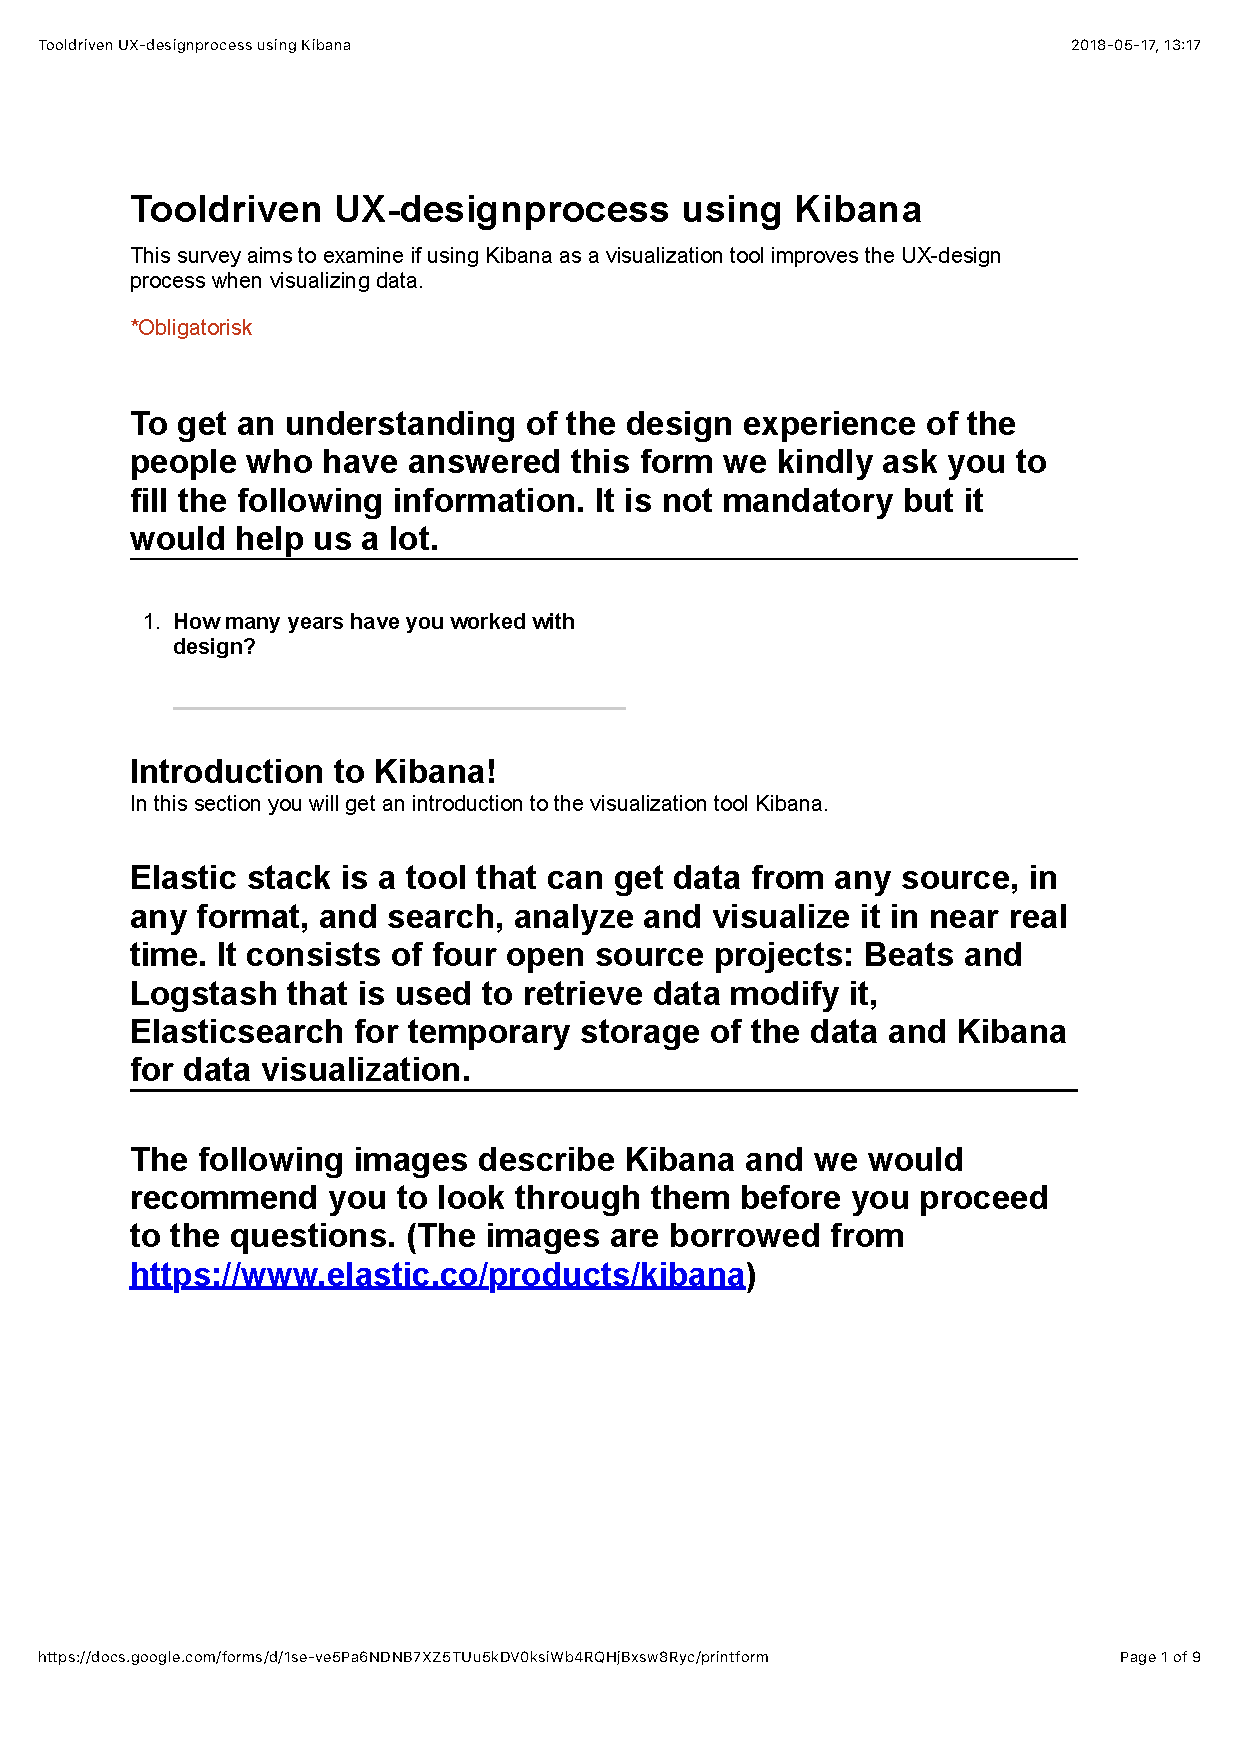
\includegraphics[width=1\textwidth]{UX_designprocess1.pdf}
\newpage
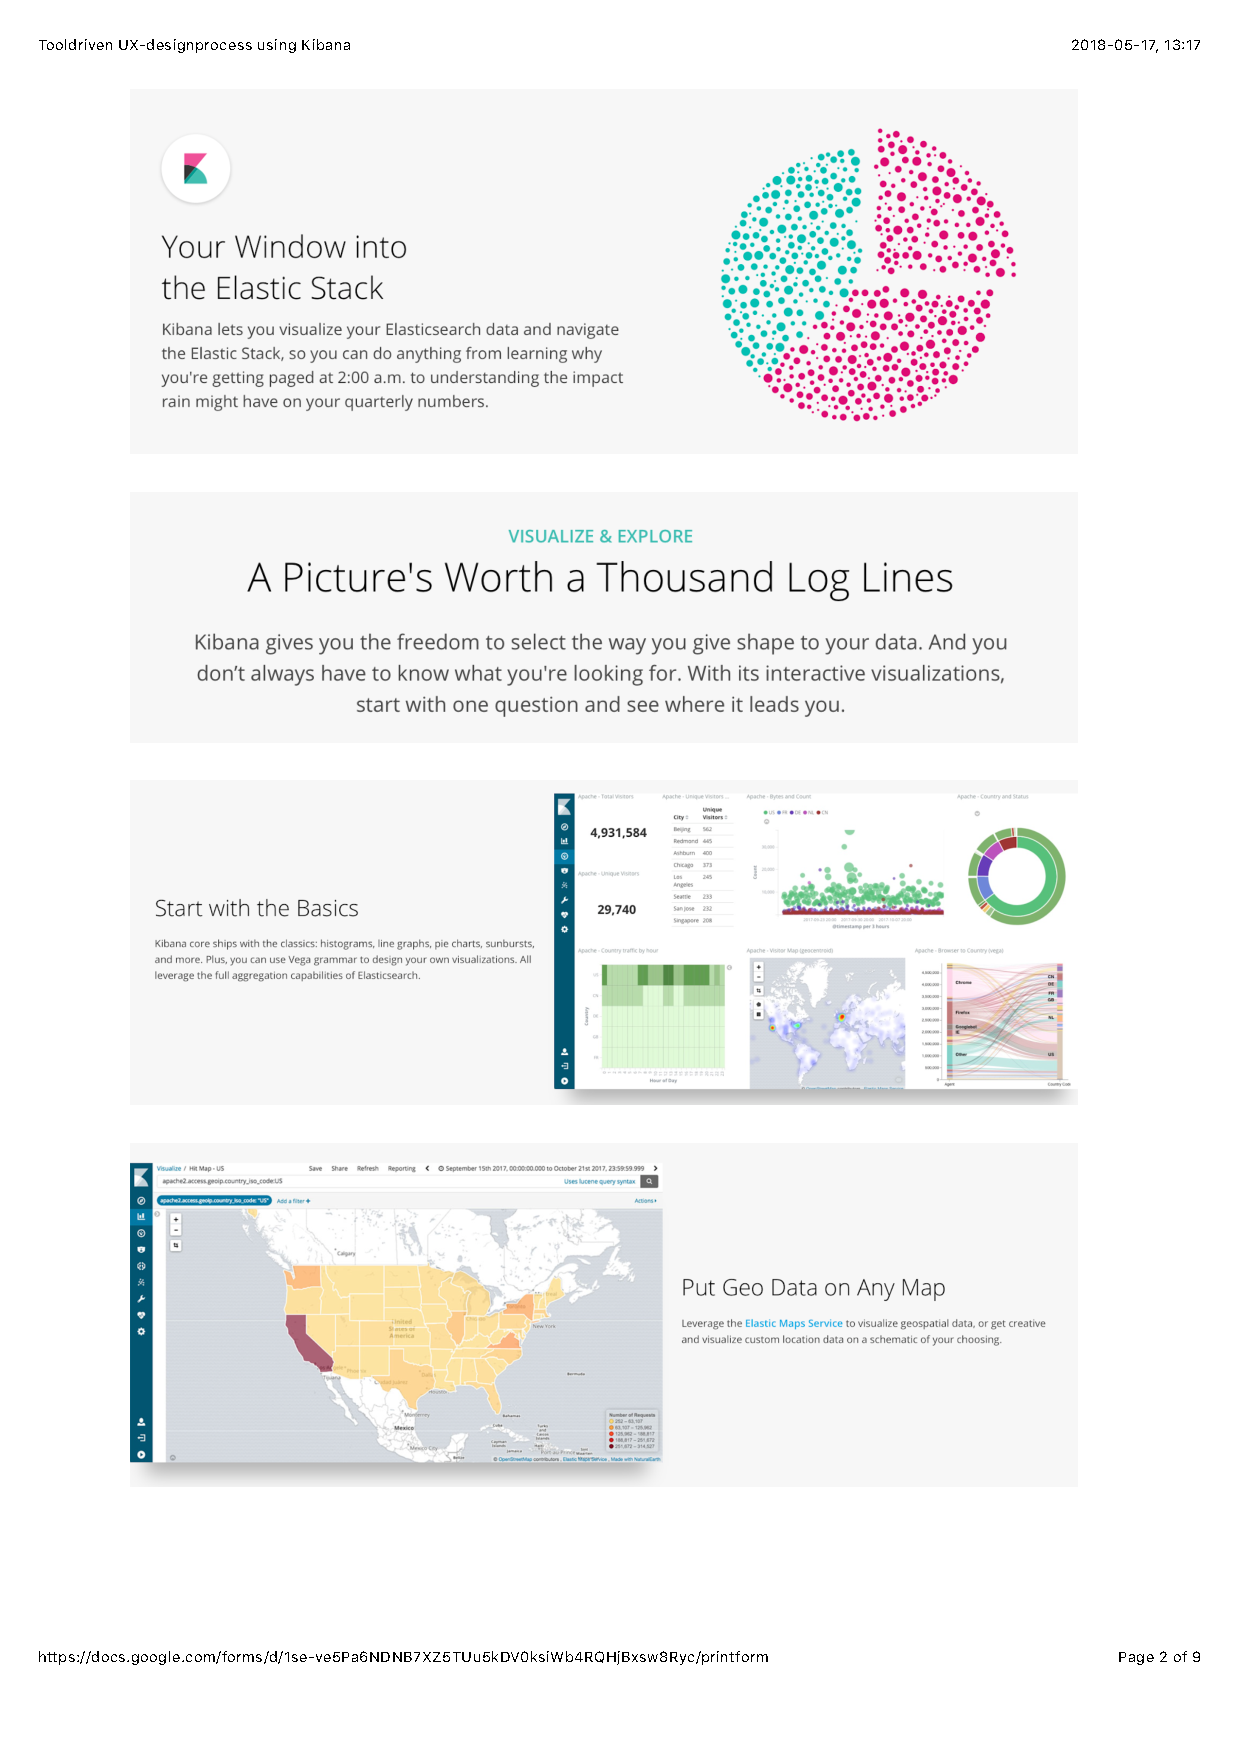
\includegraphics[width=1\textwidth]{UX_designprocess2.pdf}
\newpage
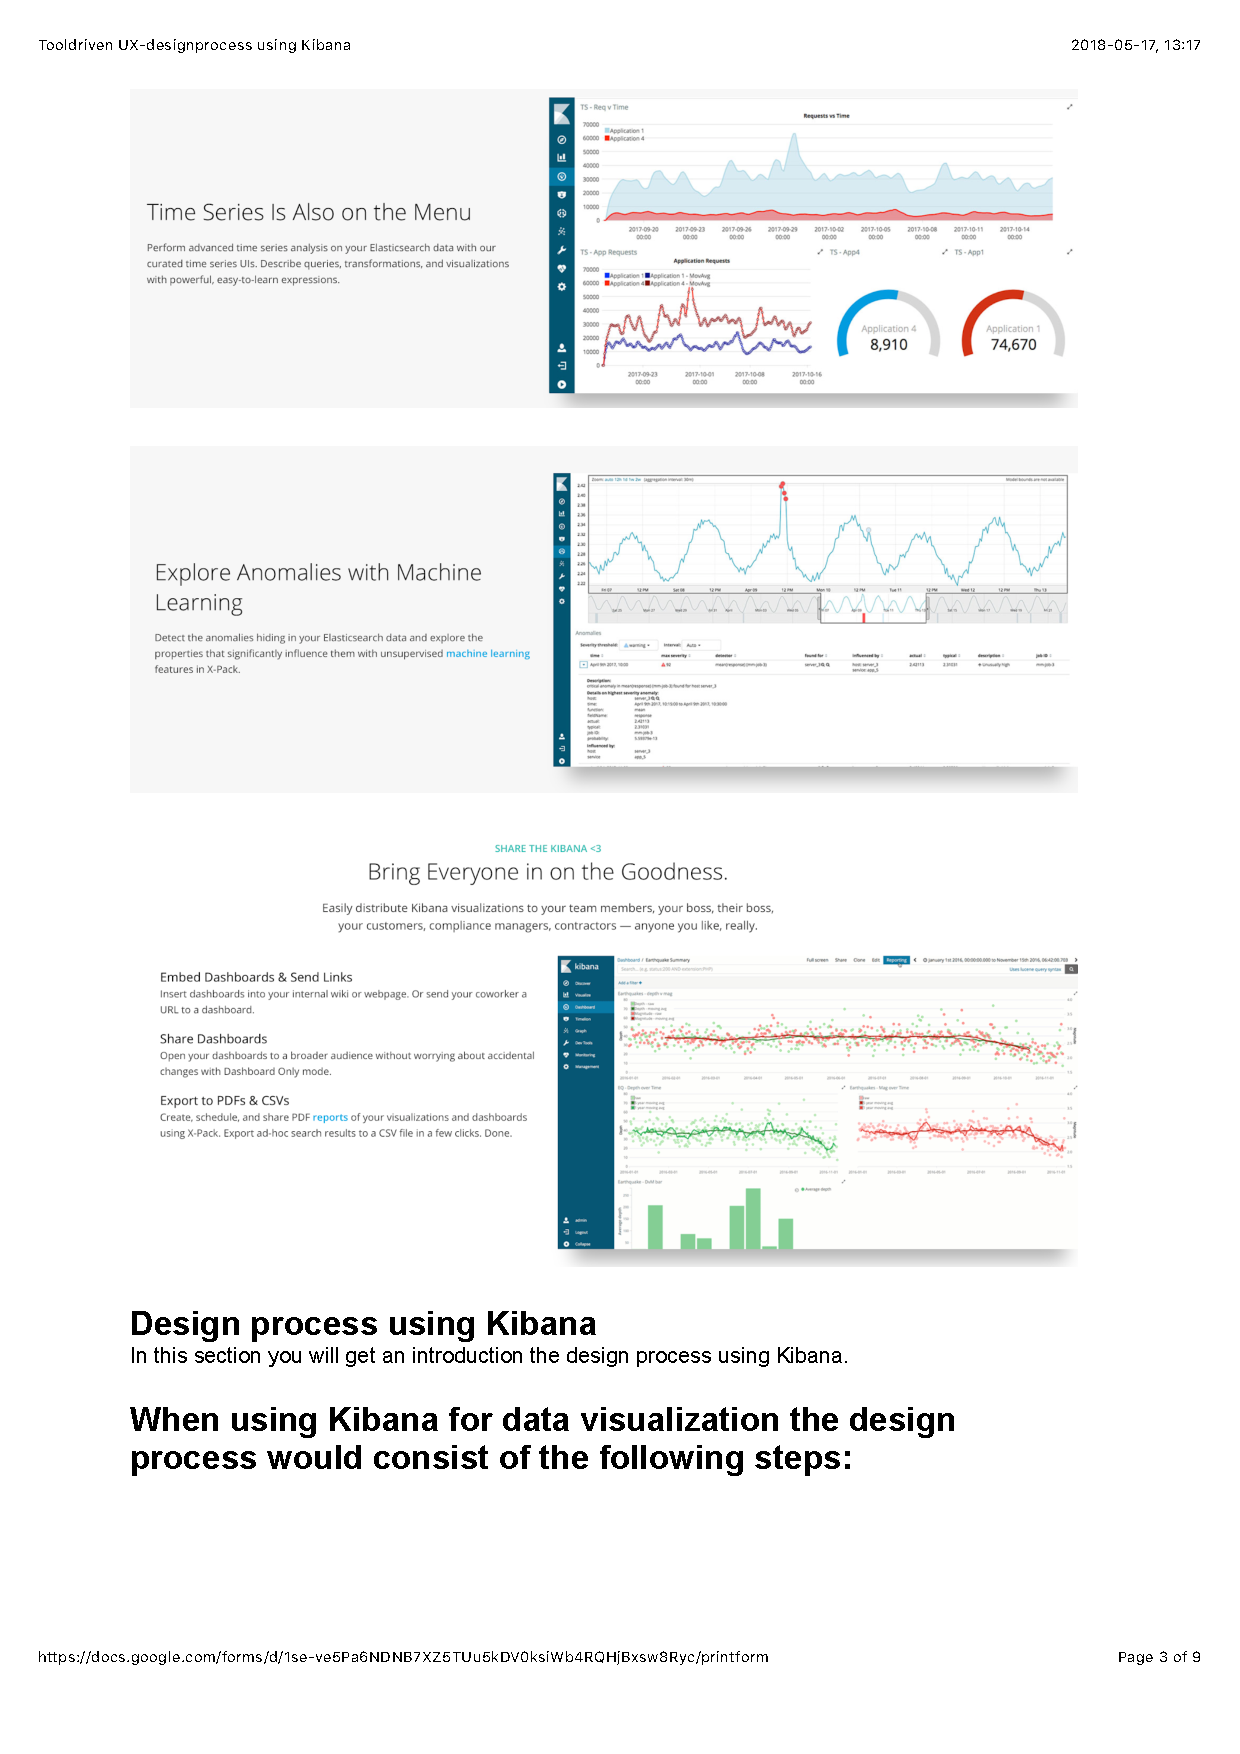
\includegraphics[width=1\textwidth]{UX_designprocess3.pdf}
\newpage
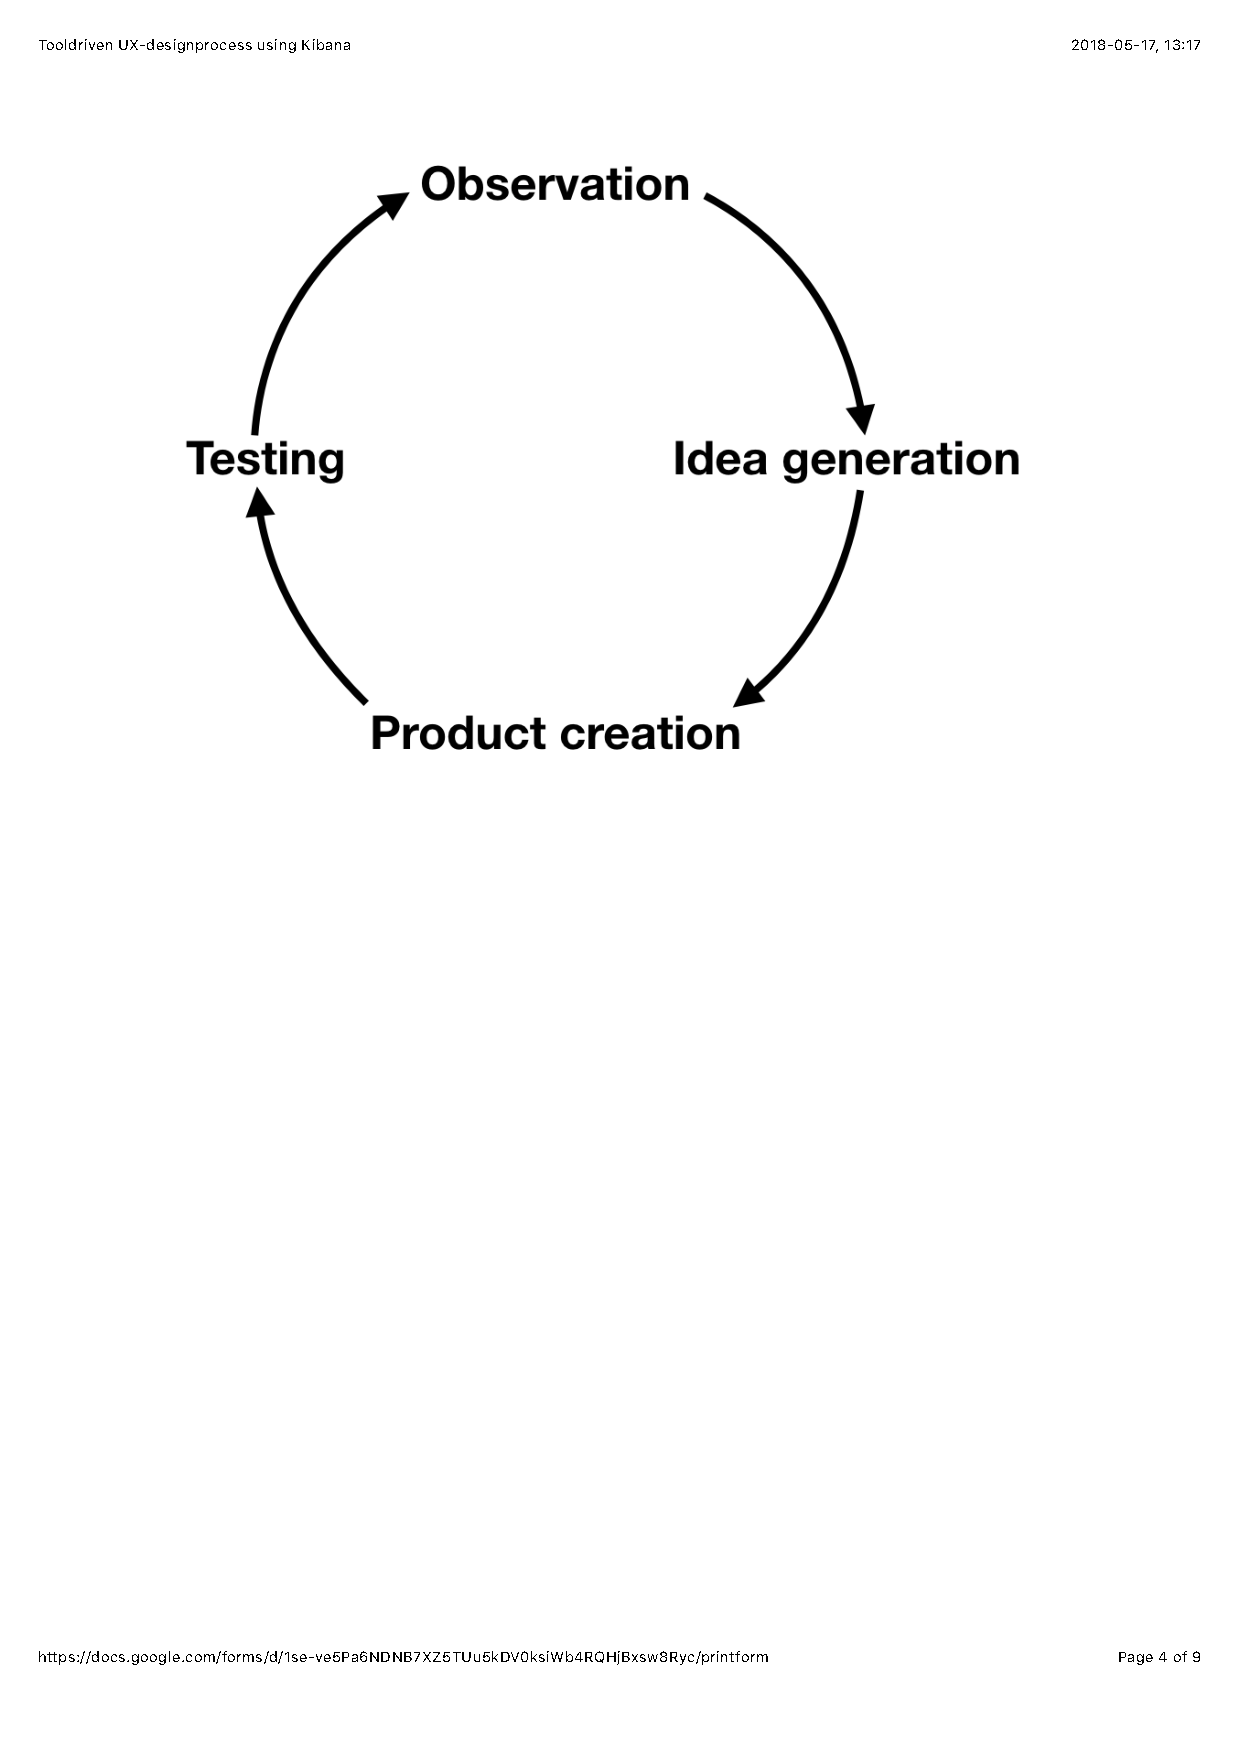
\includegraphics[width=1\textwidth]{UX_designprocess4.pdf}
\newpage
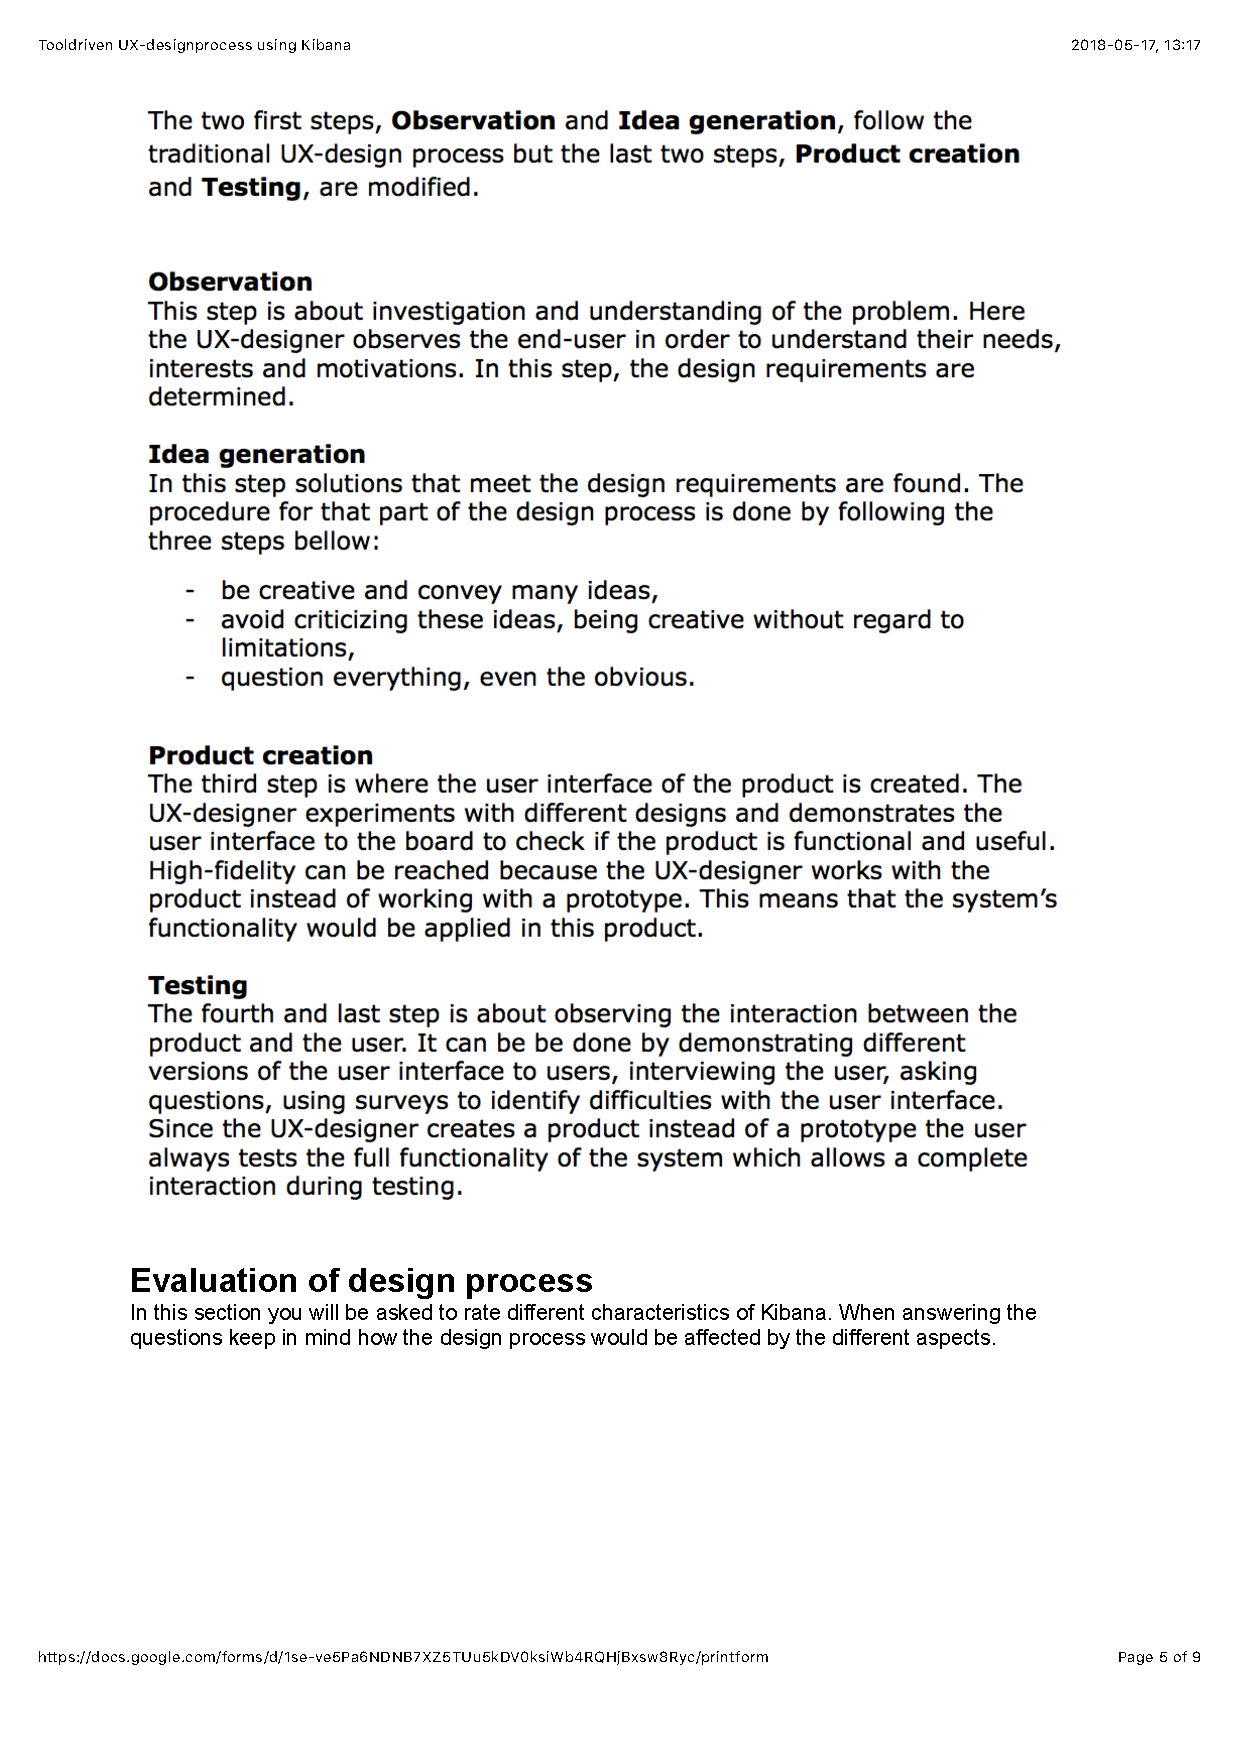
\includegraphics[width=1\textwidth]{UX_designprocess5.pdf}
\newpage
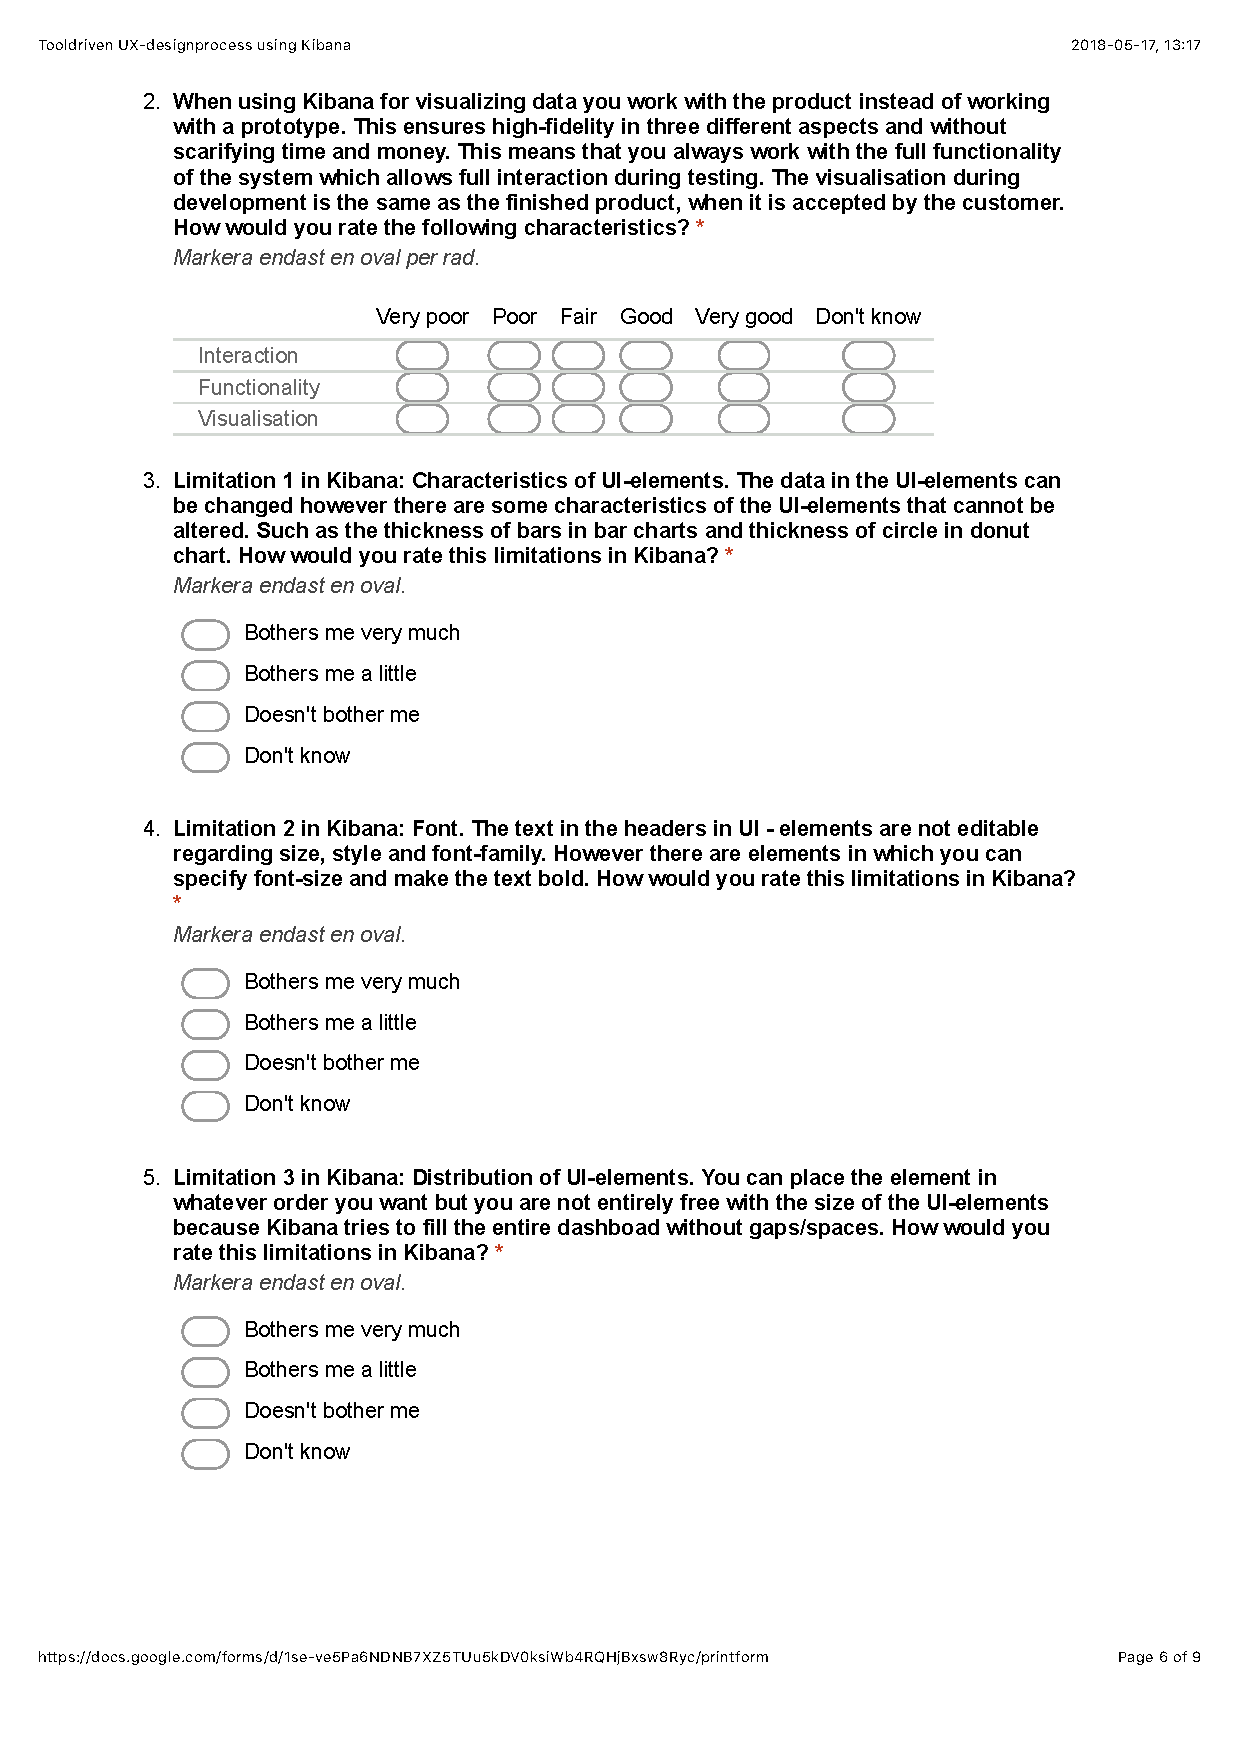
\includegraphics[width=1\textwidth]{UX_designprocess6.pdf}
\newpage
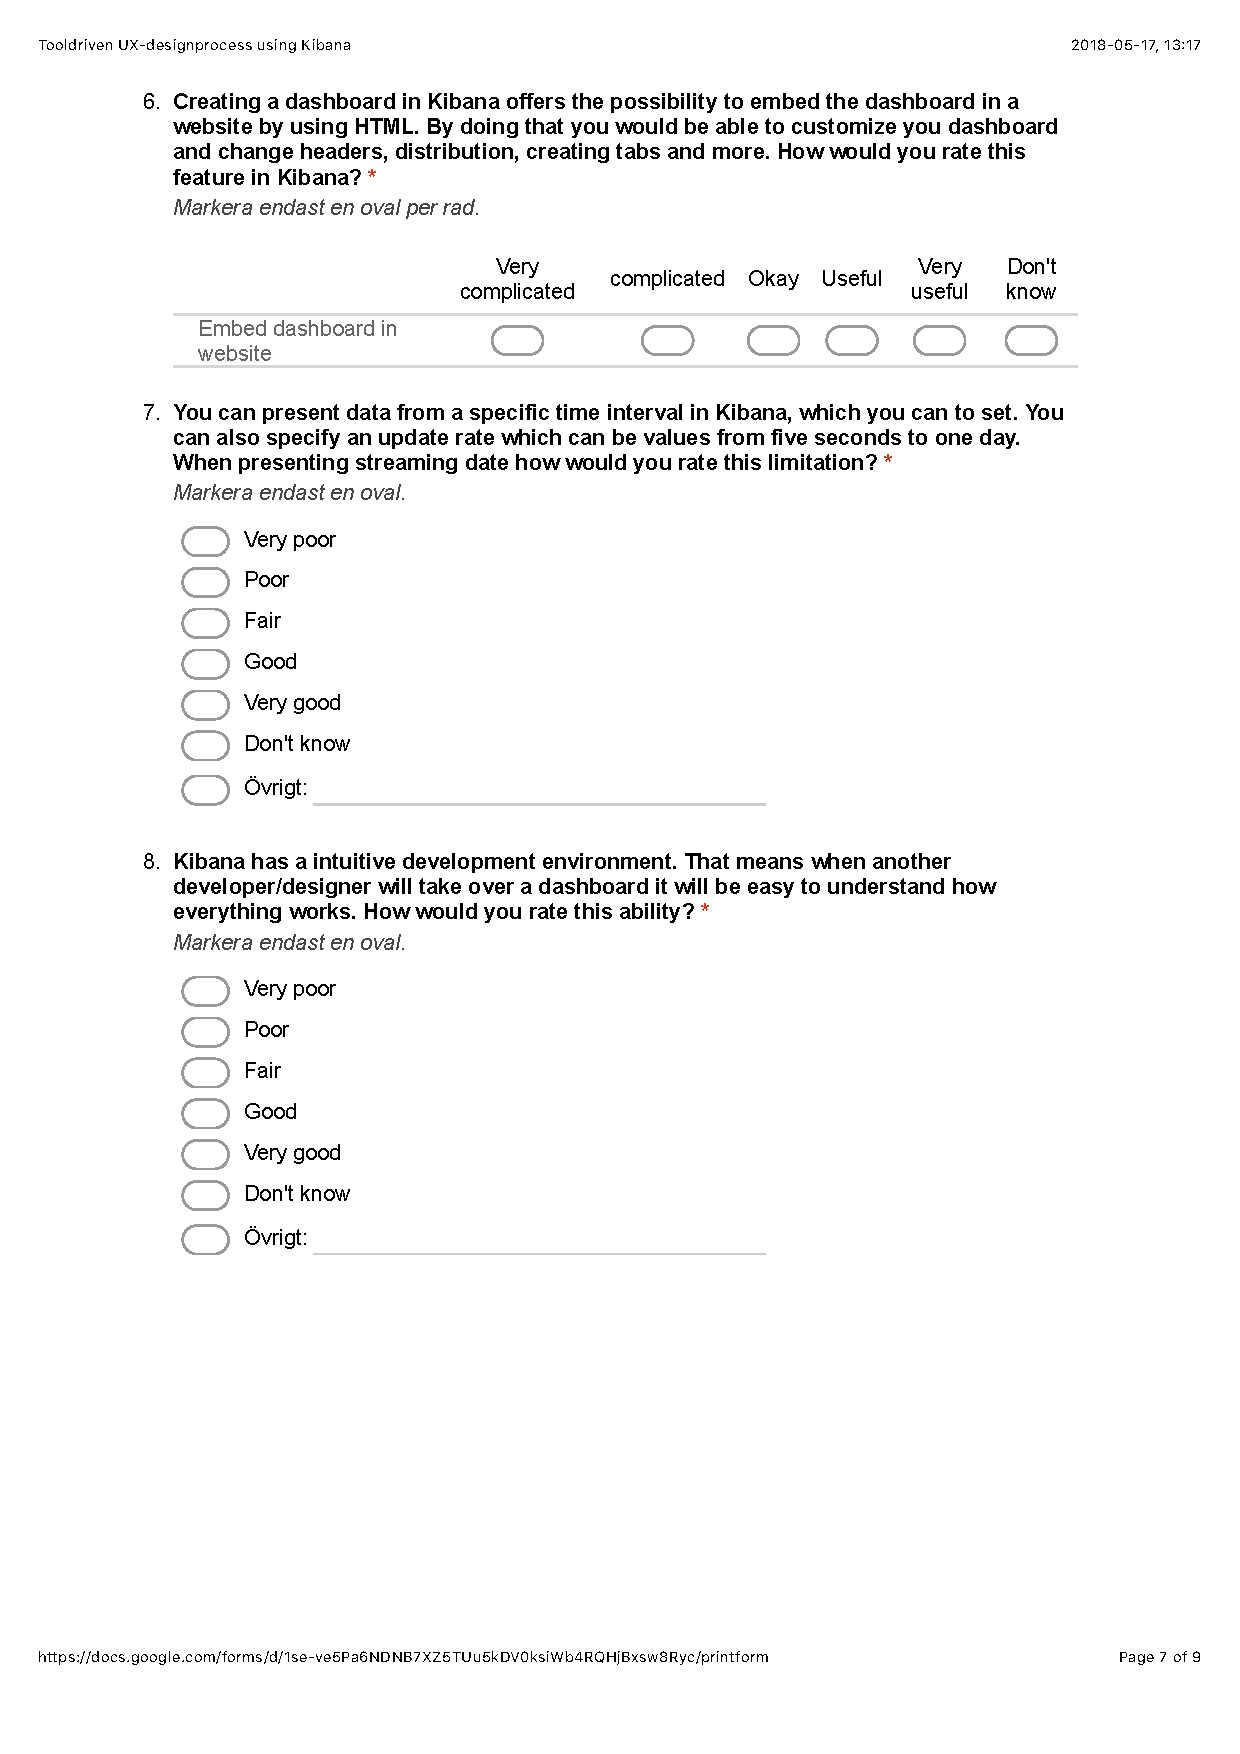
\includegraphics[width=1\textwidth]{UX_designprocess7.pdf}
\newpage
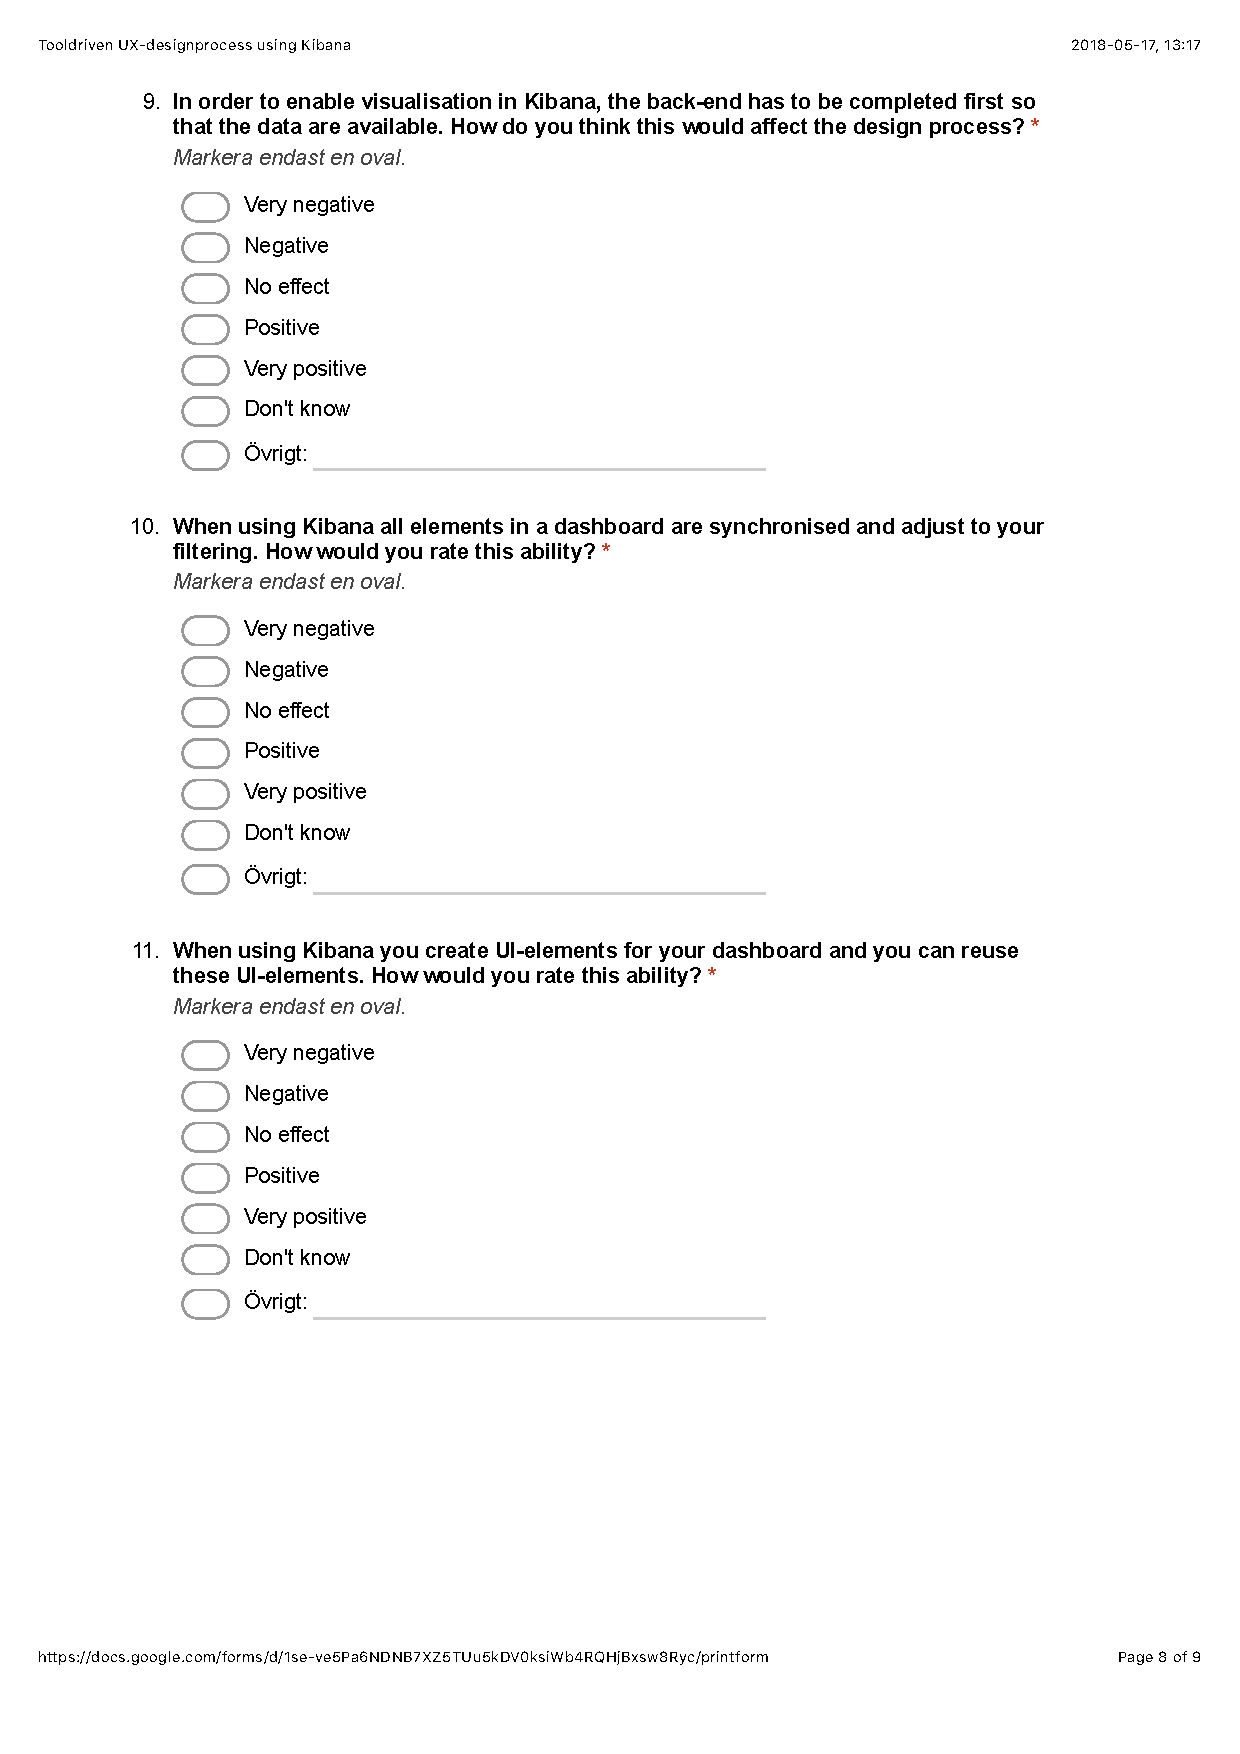
\includegraphics[width=1\textwidth]{UX_designprocess8.pdf}
\newpage
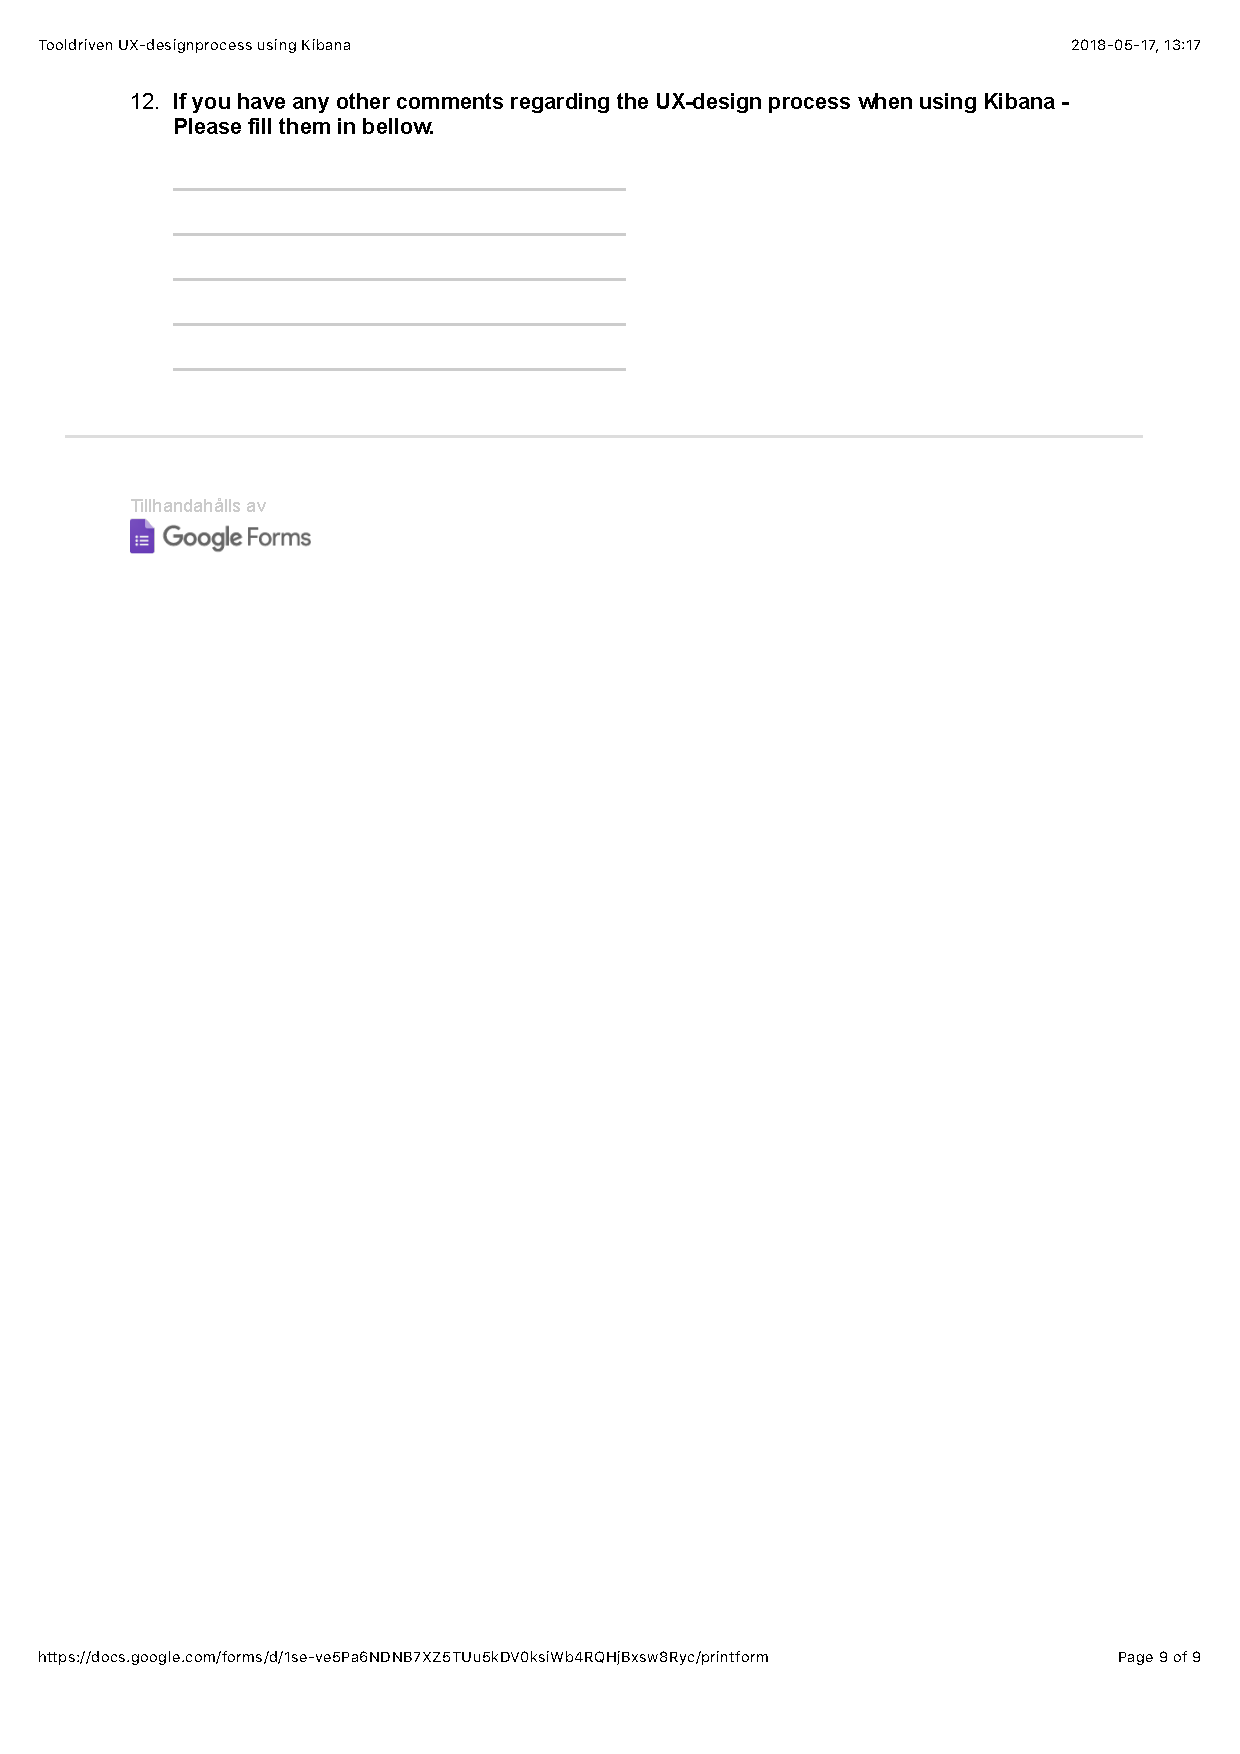
\includegraphics[width=1\textwidth]{UX_designprocess9.pdf}

\section{Personas}
\subsection{Curious Carl}
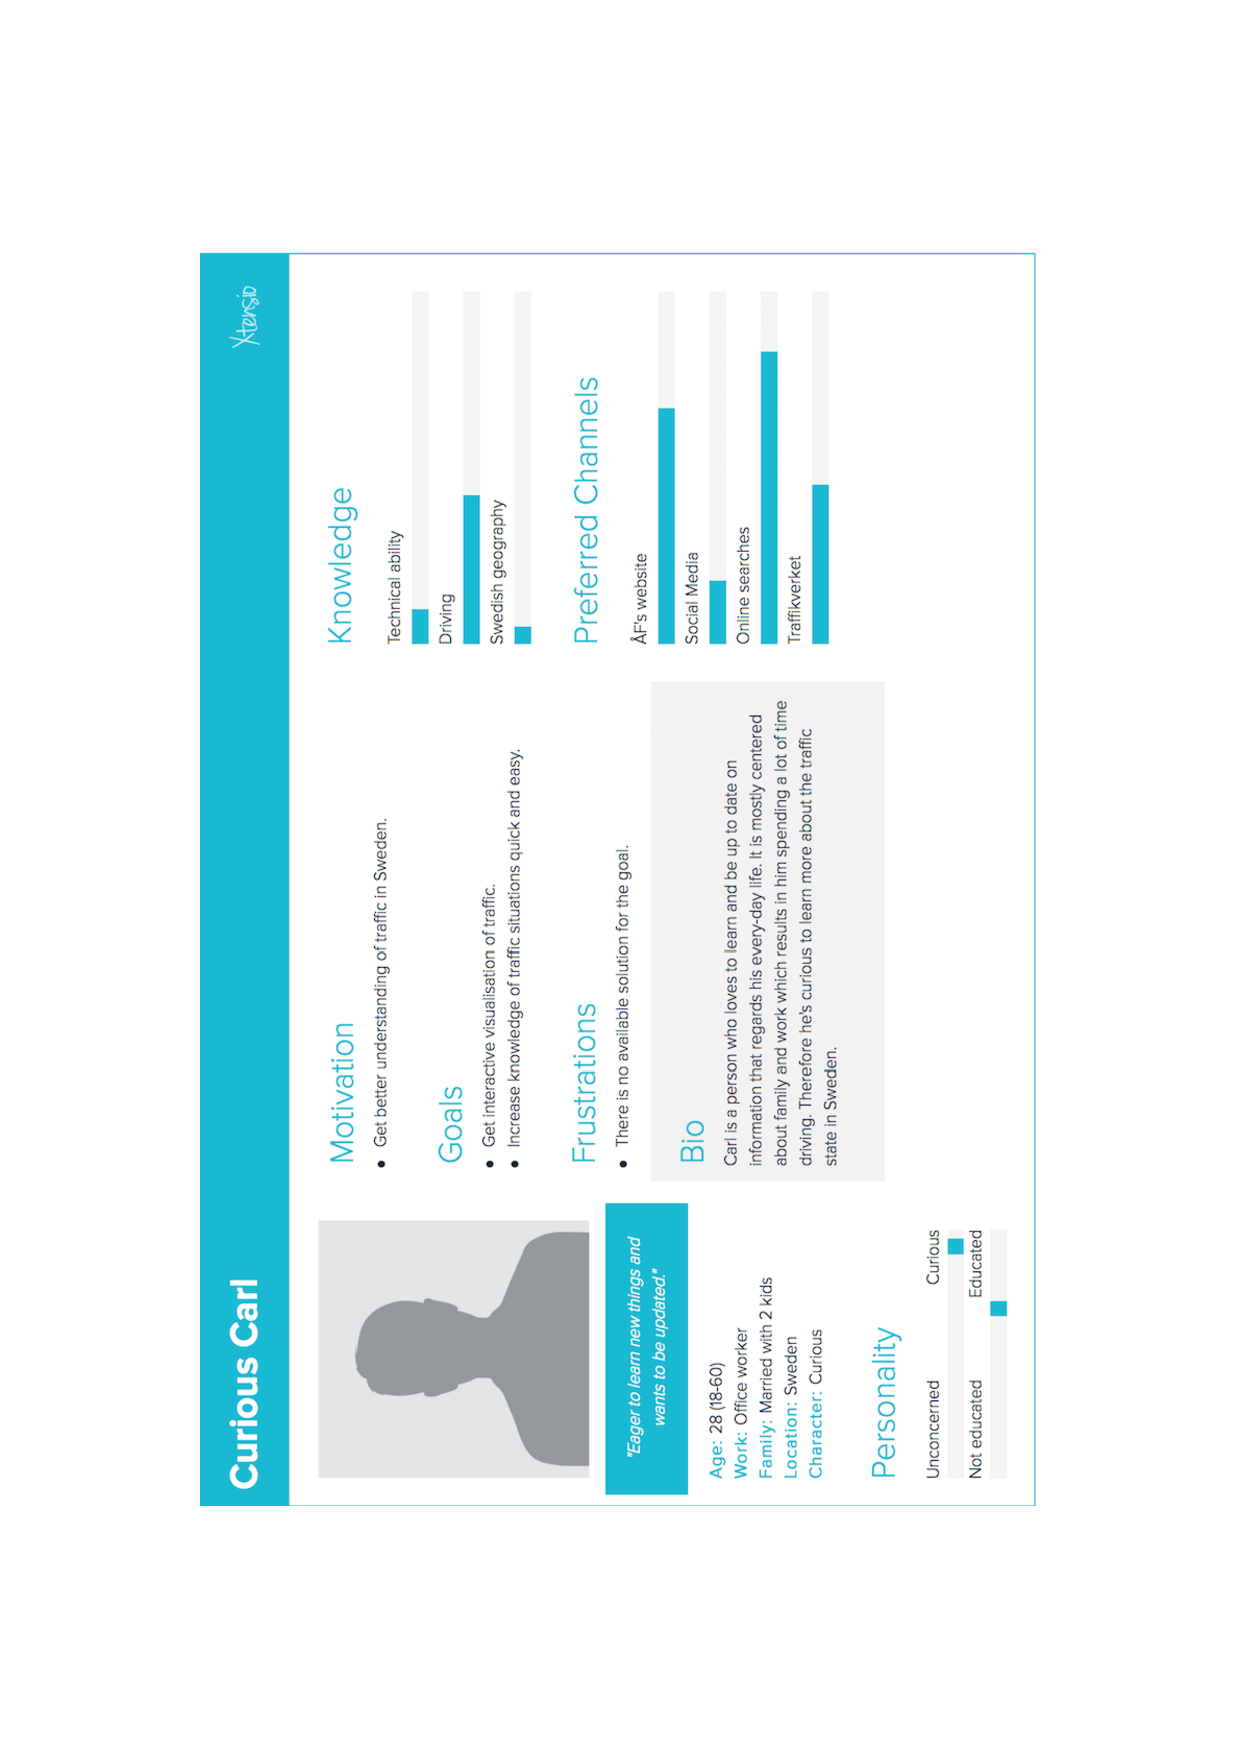
\includegraphics[width=1\textwidth]{CuriousCarl}

\subsection{Wondering Walter}
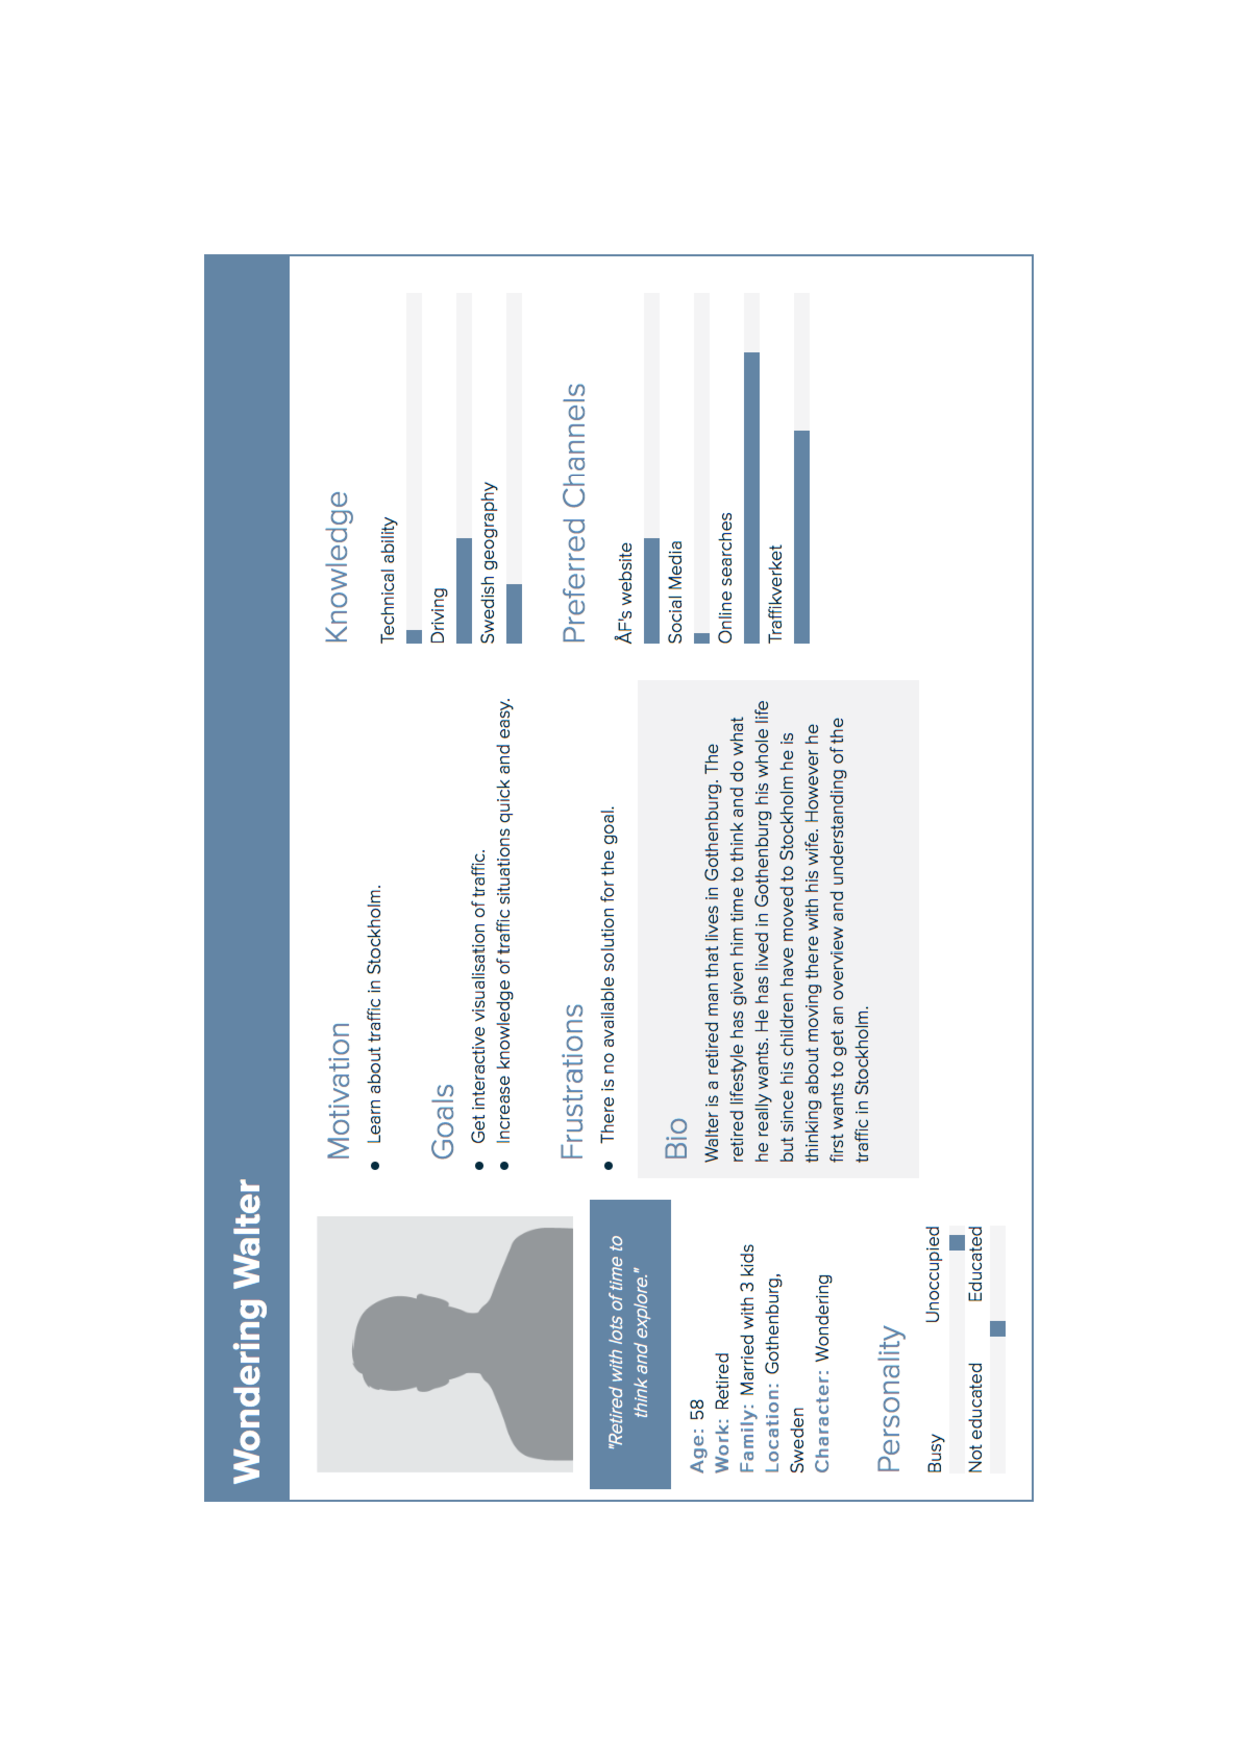
\includegraphics[width=1\textwidth]{WonderingWalter}
\newpage
\subsection{Analyze Alice}
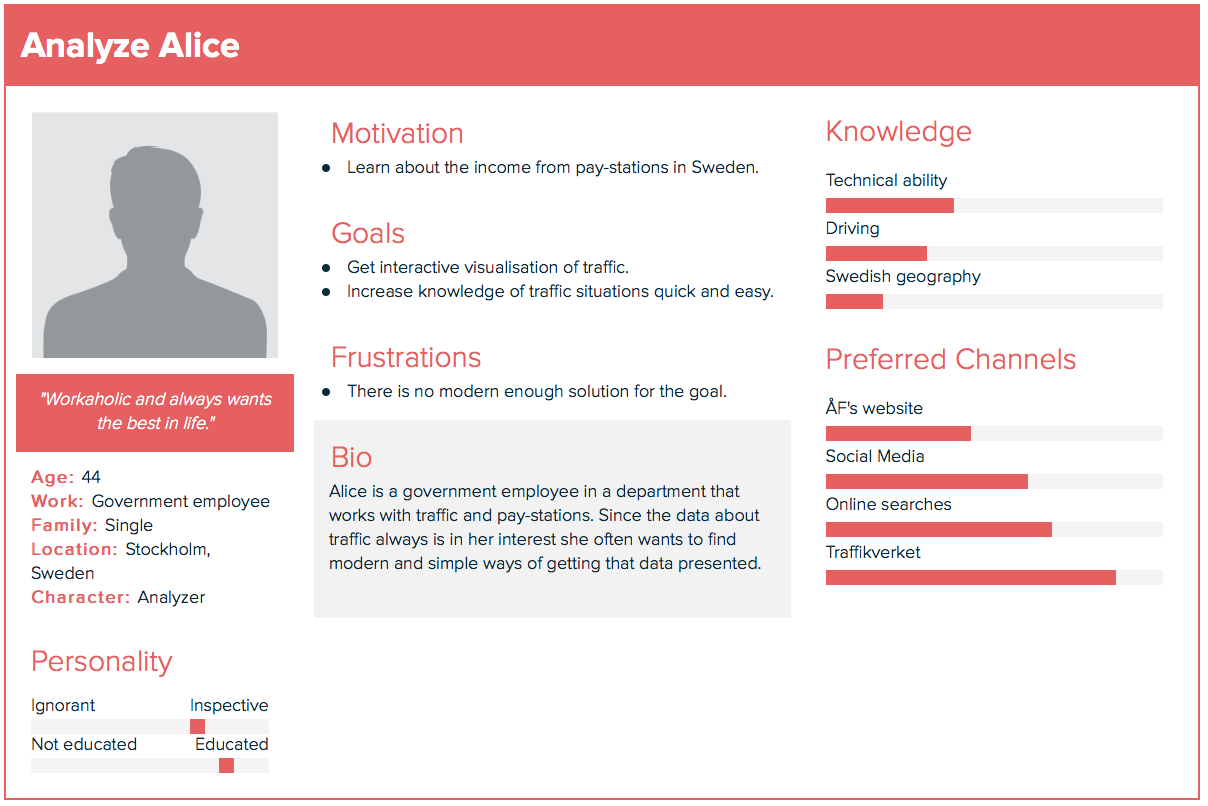
\includegraphics[width=1\textwidth]{AnalyzeAlice}

\section{Testningsformulär}
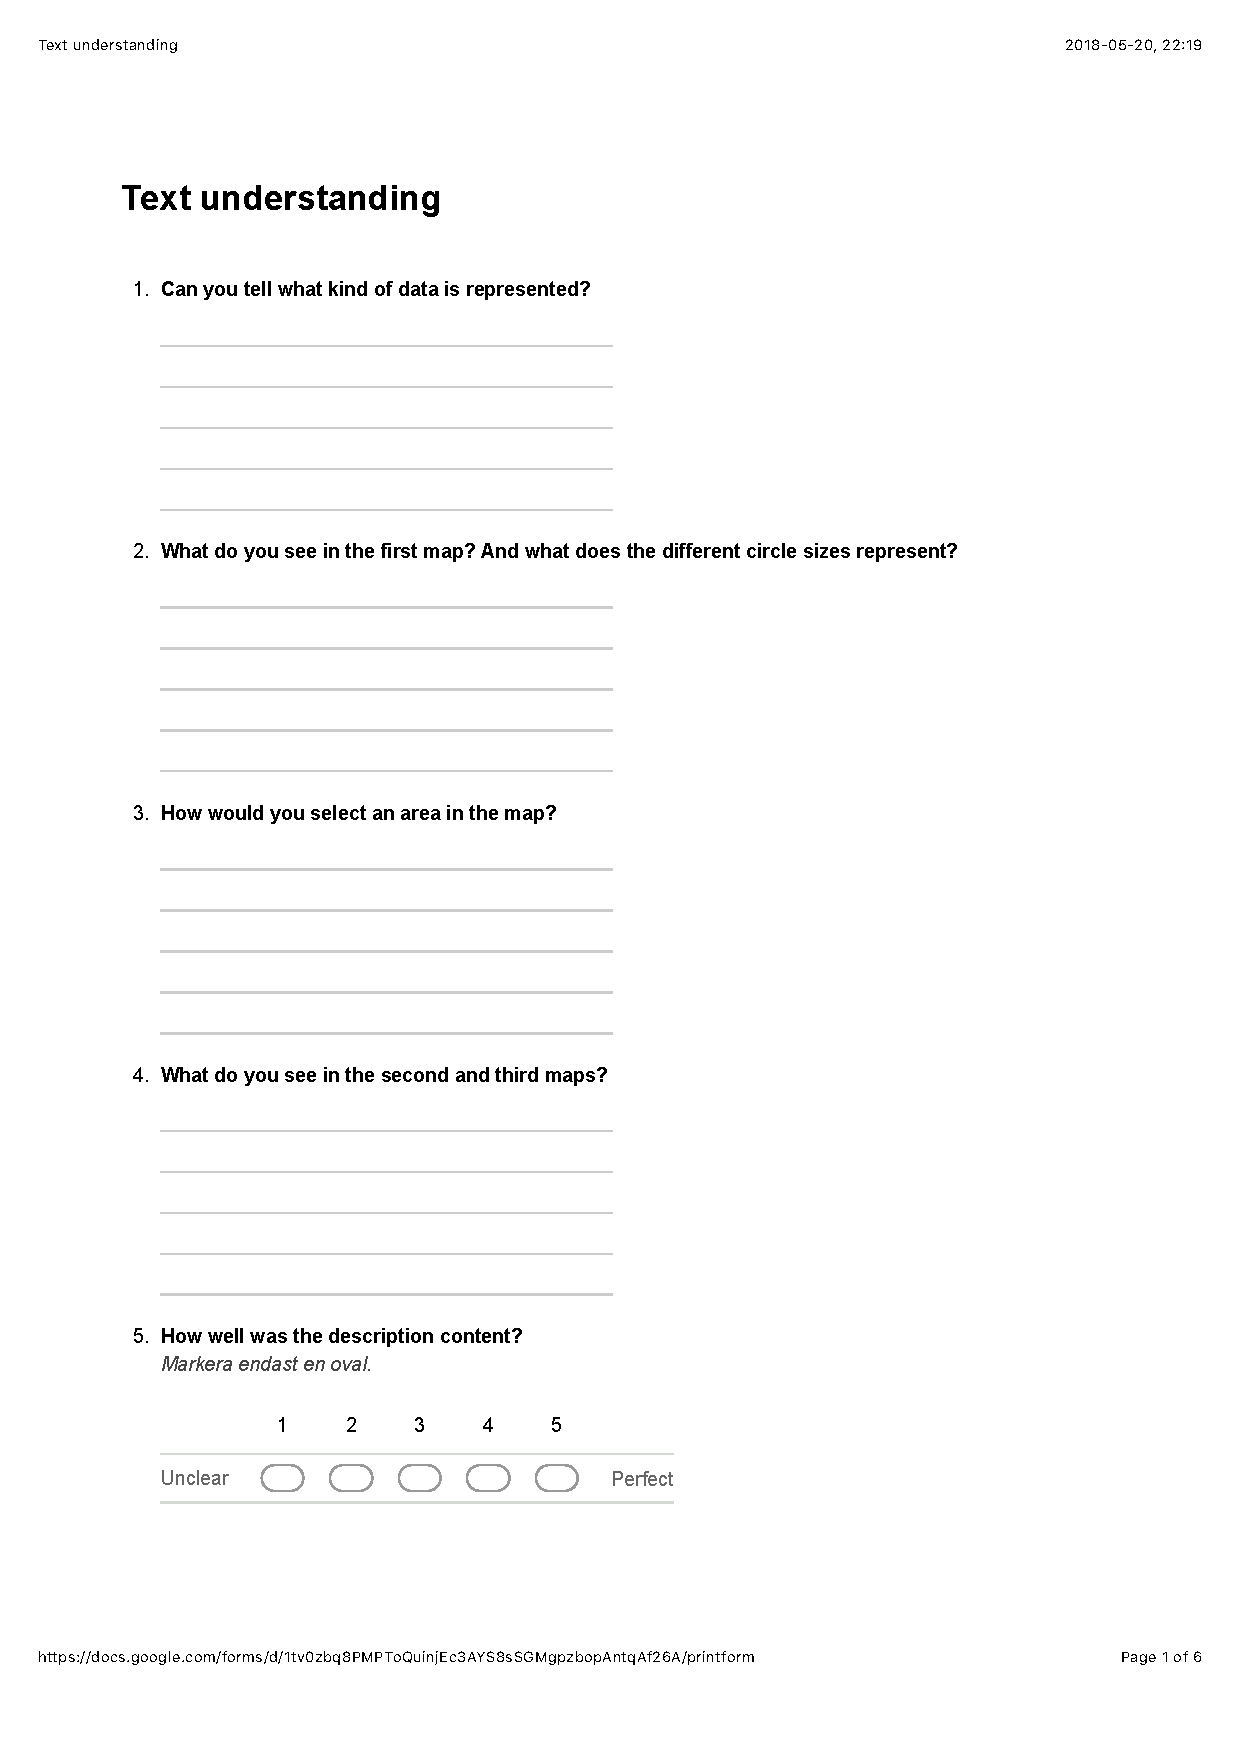
\includegraphics[width=1\textwidth]{TextUnderstanding1.pdf}
\newpage
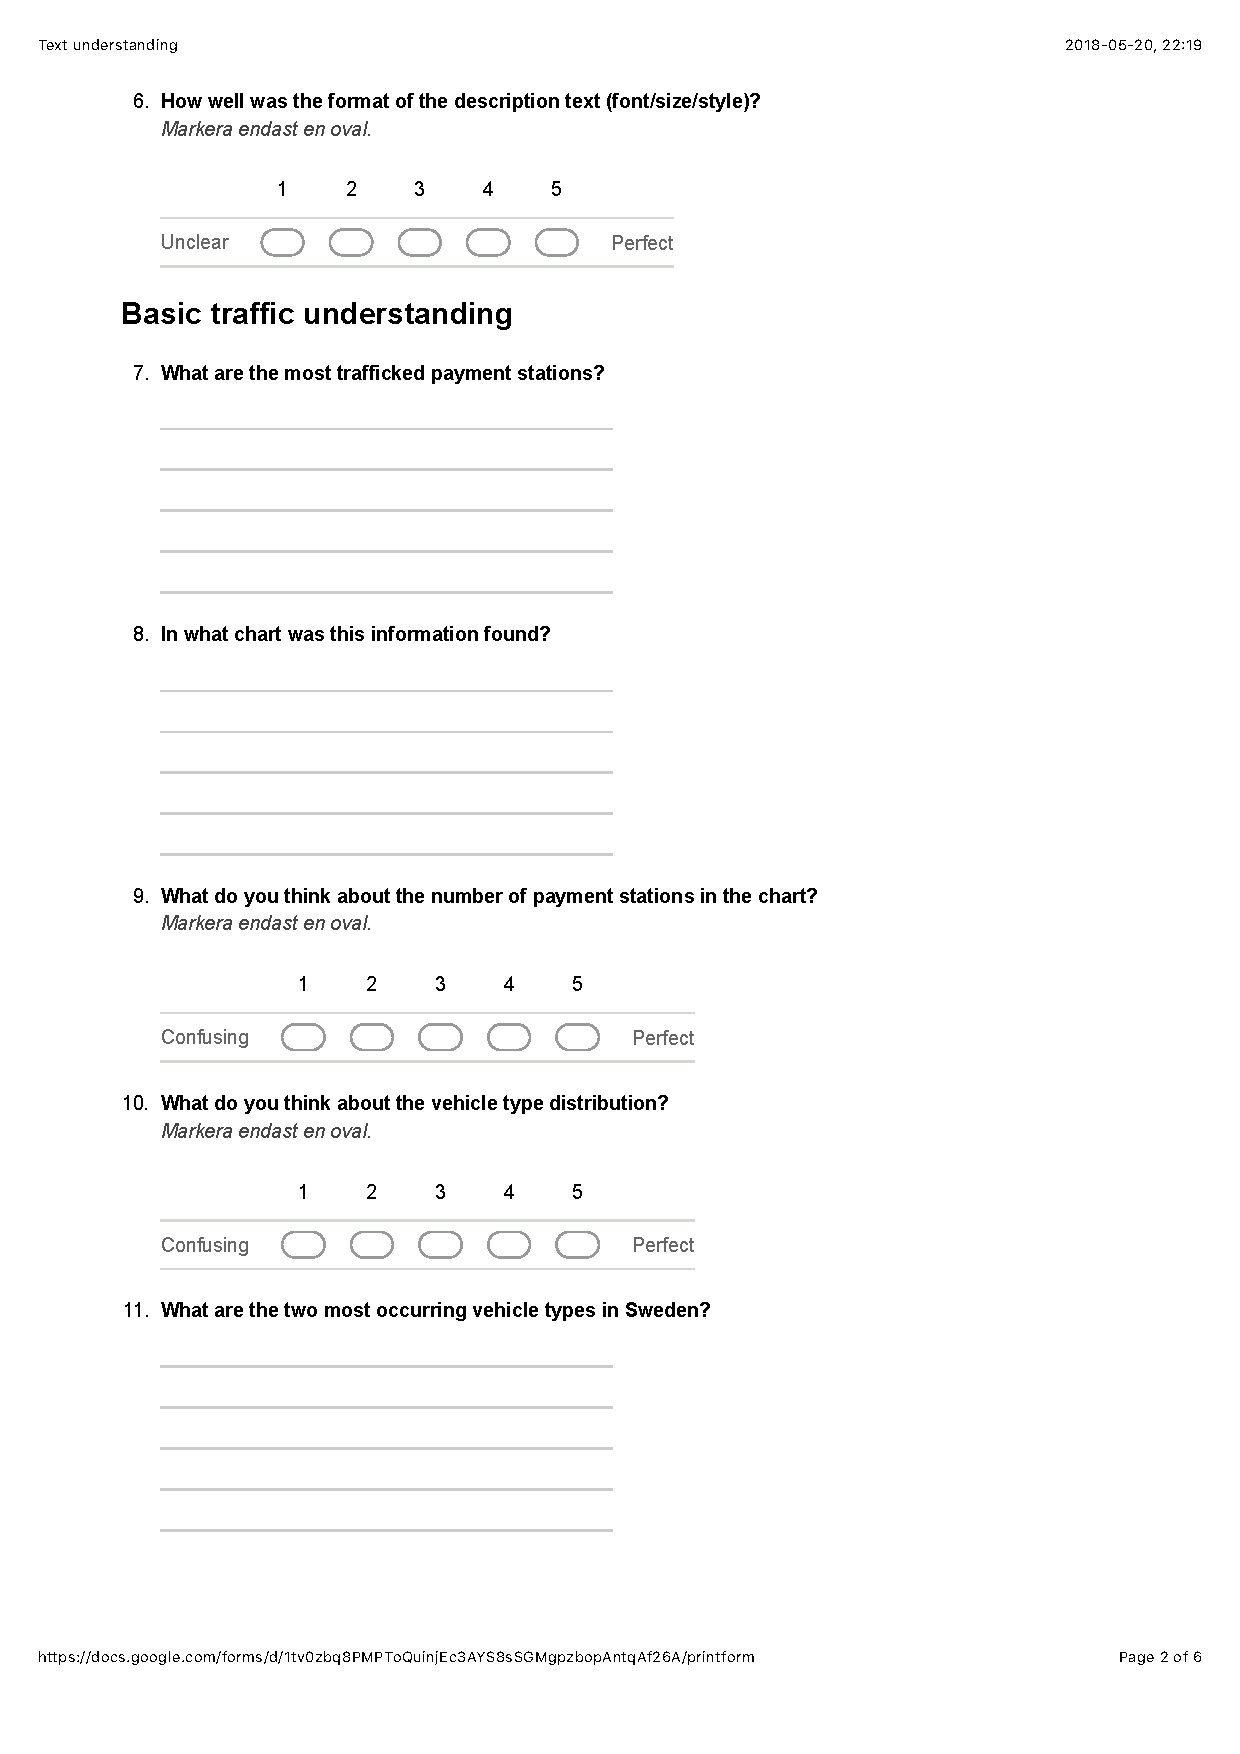
\includegraphics[width=1\textwidth]{TextUnderstanding2.pdf}
\newpage
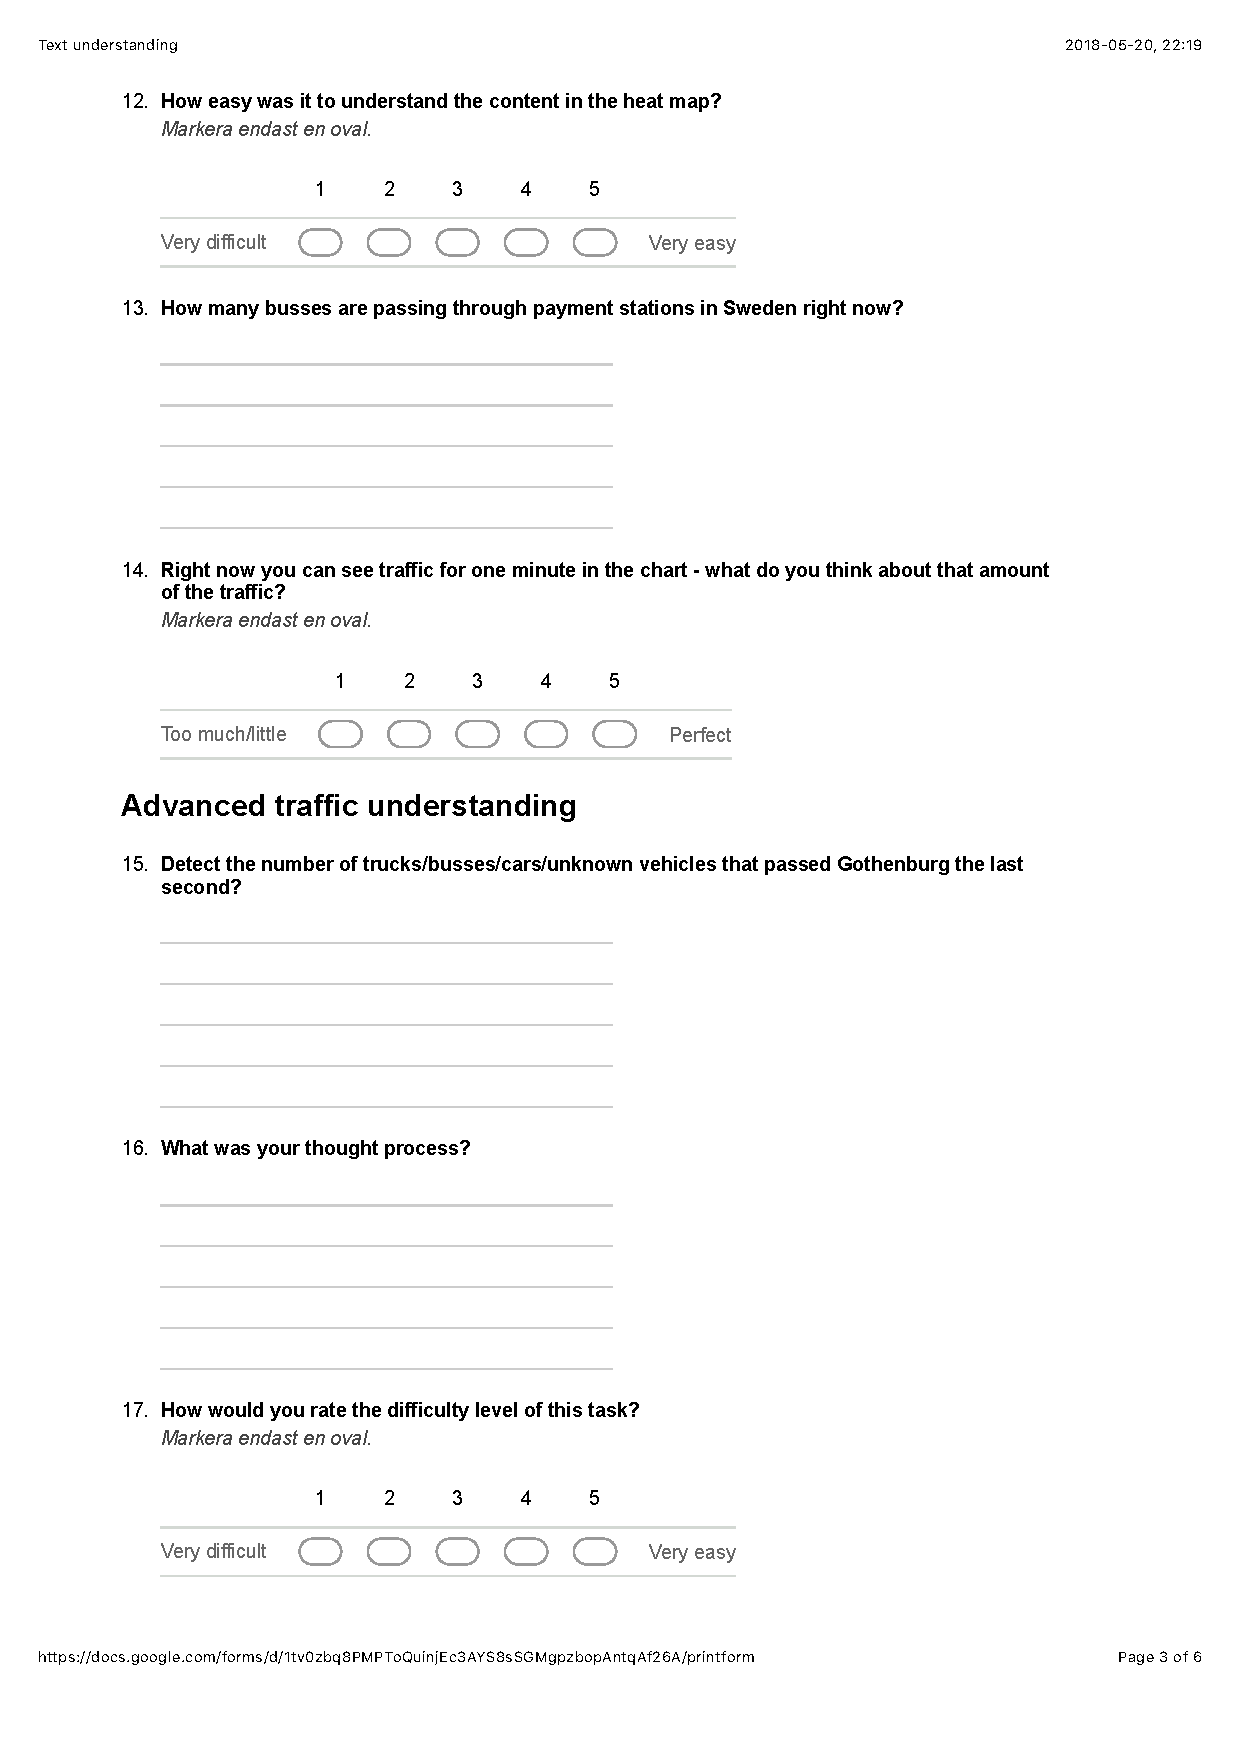
\includegraphics[width=1\textwidth]{TextUnderstanding3.pdf}
\newpage
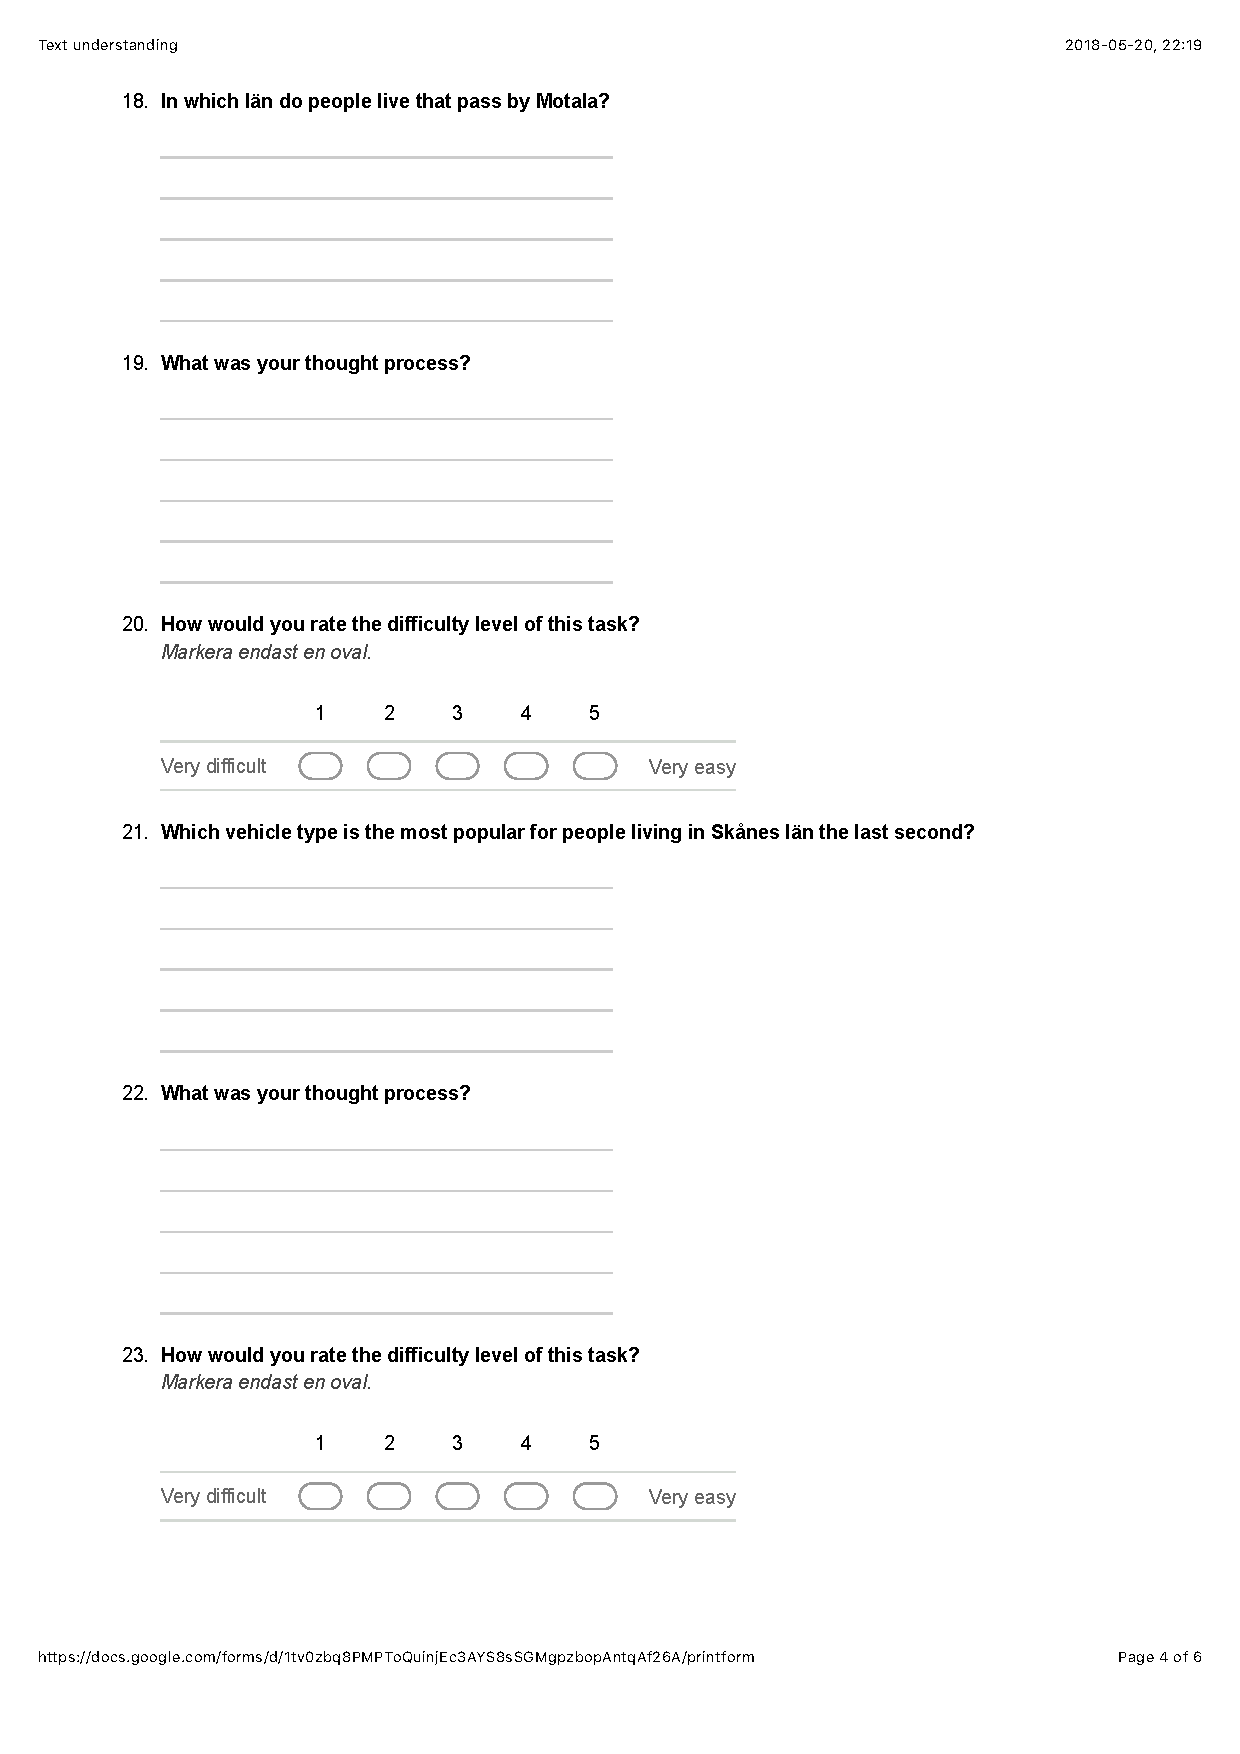
\includegraphics[width=1\textwidth]{TextUnderstanding4.pdf}
\newpage
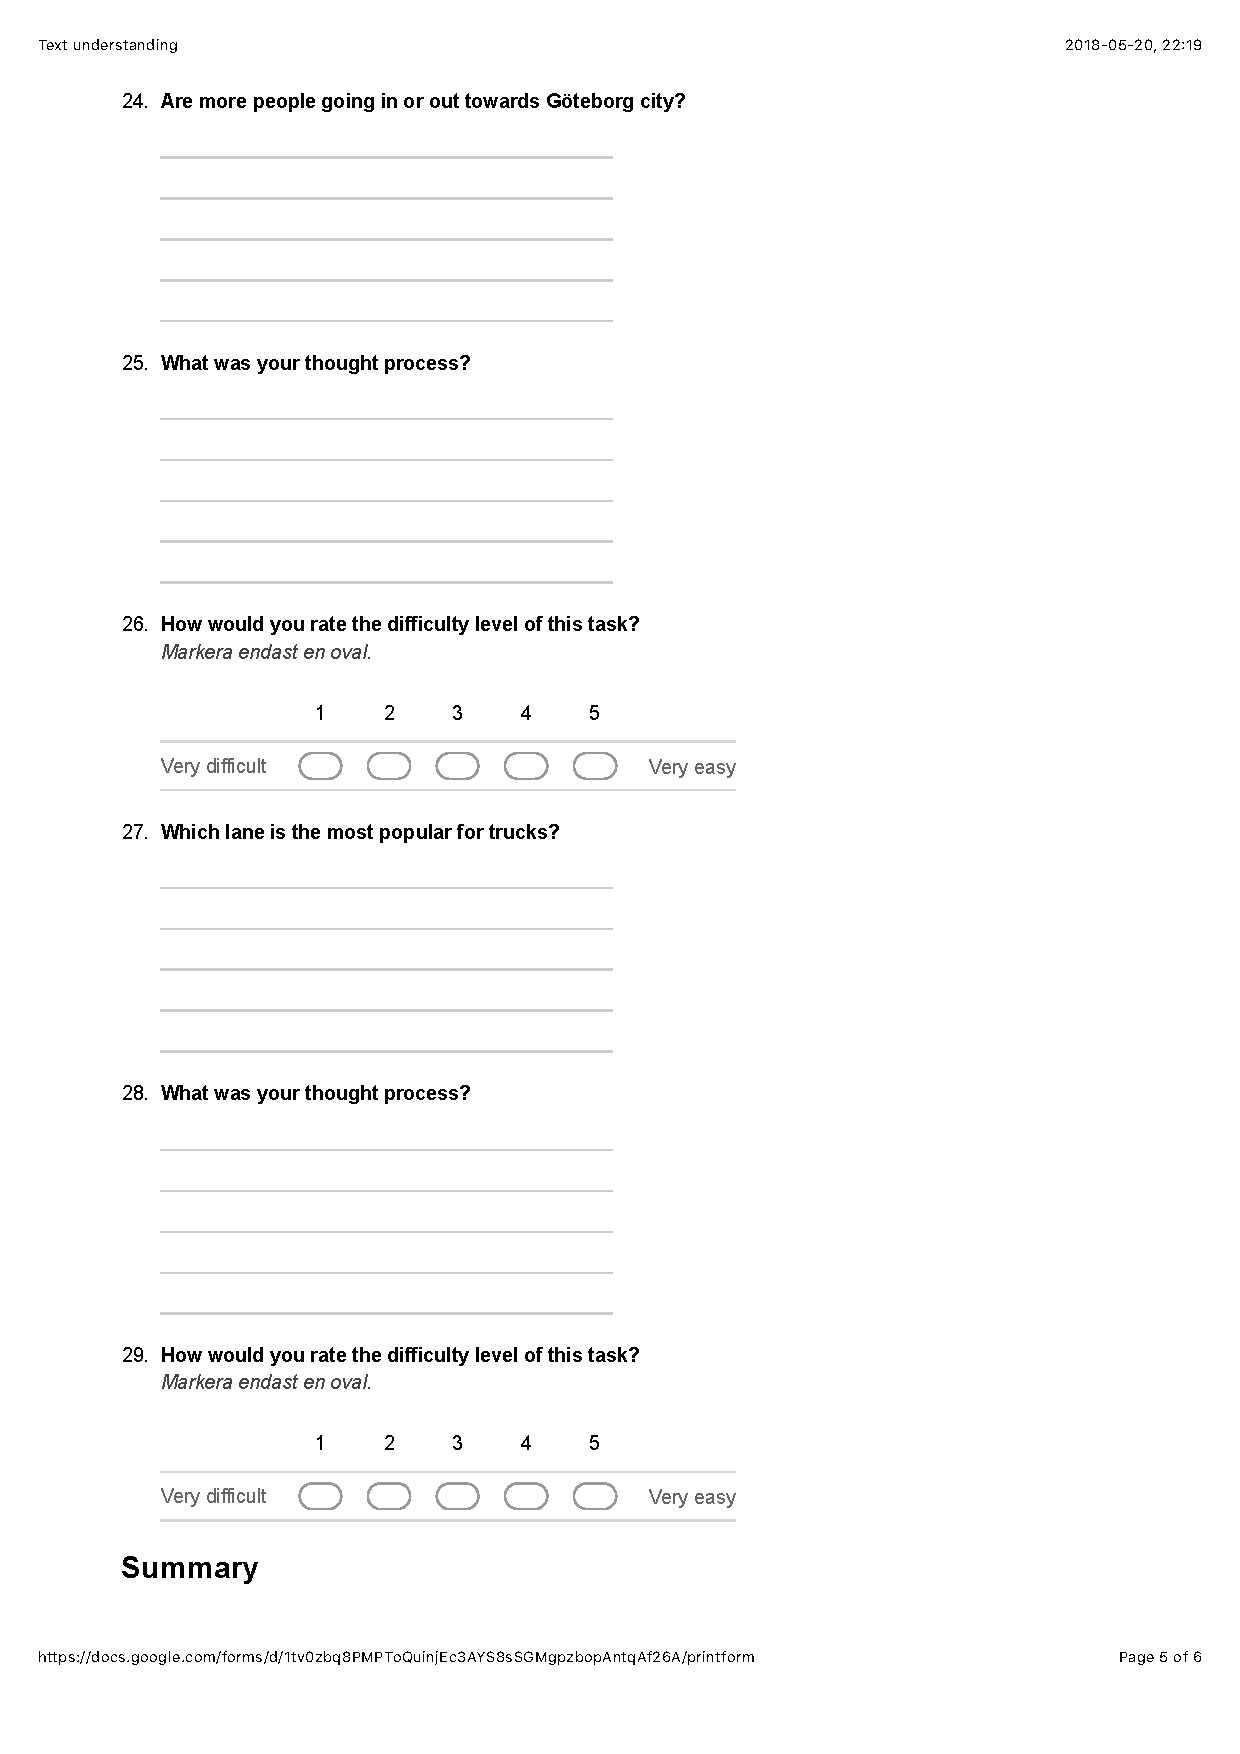
\includegraphics[width=1\textwidth]{TextUnderstanding5.pdf}
\newpage
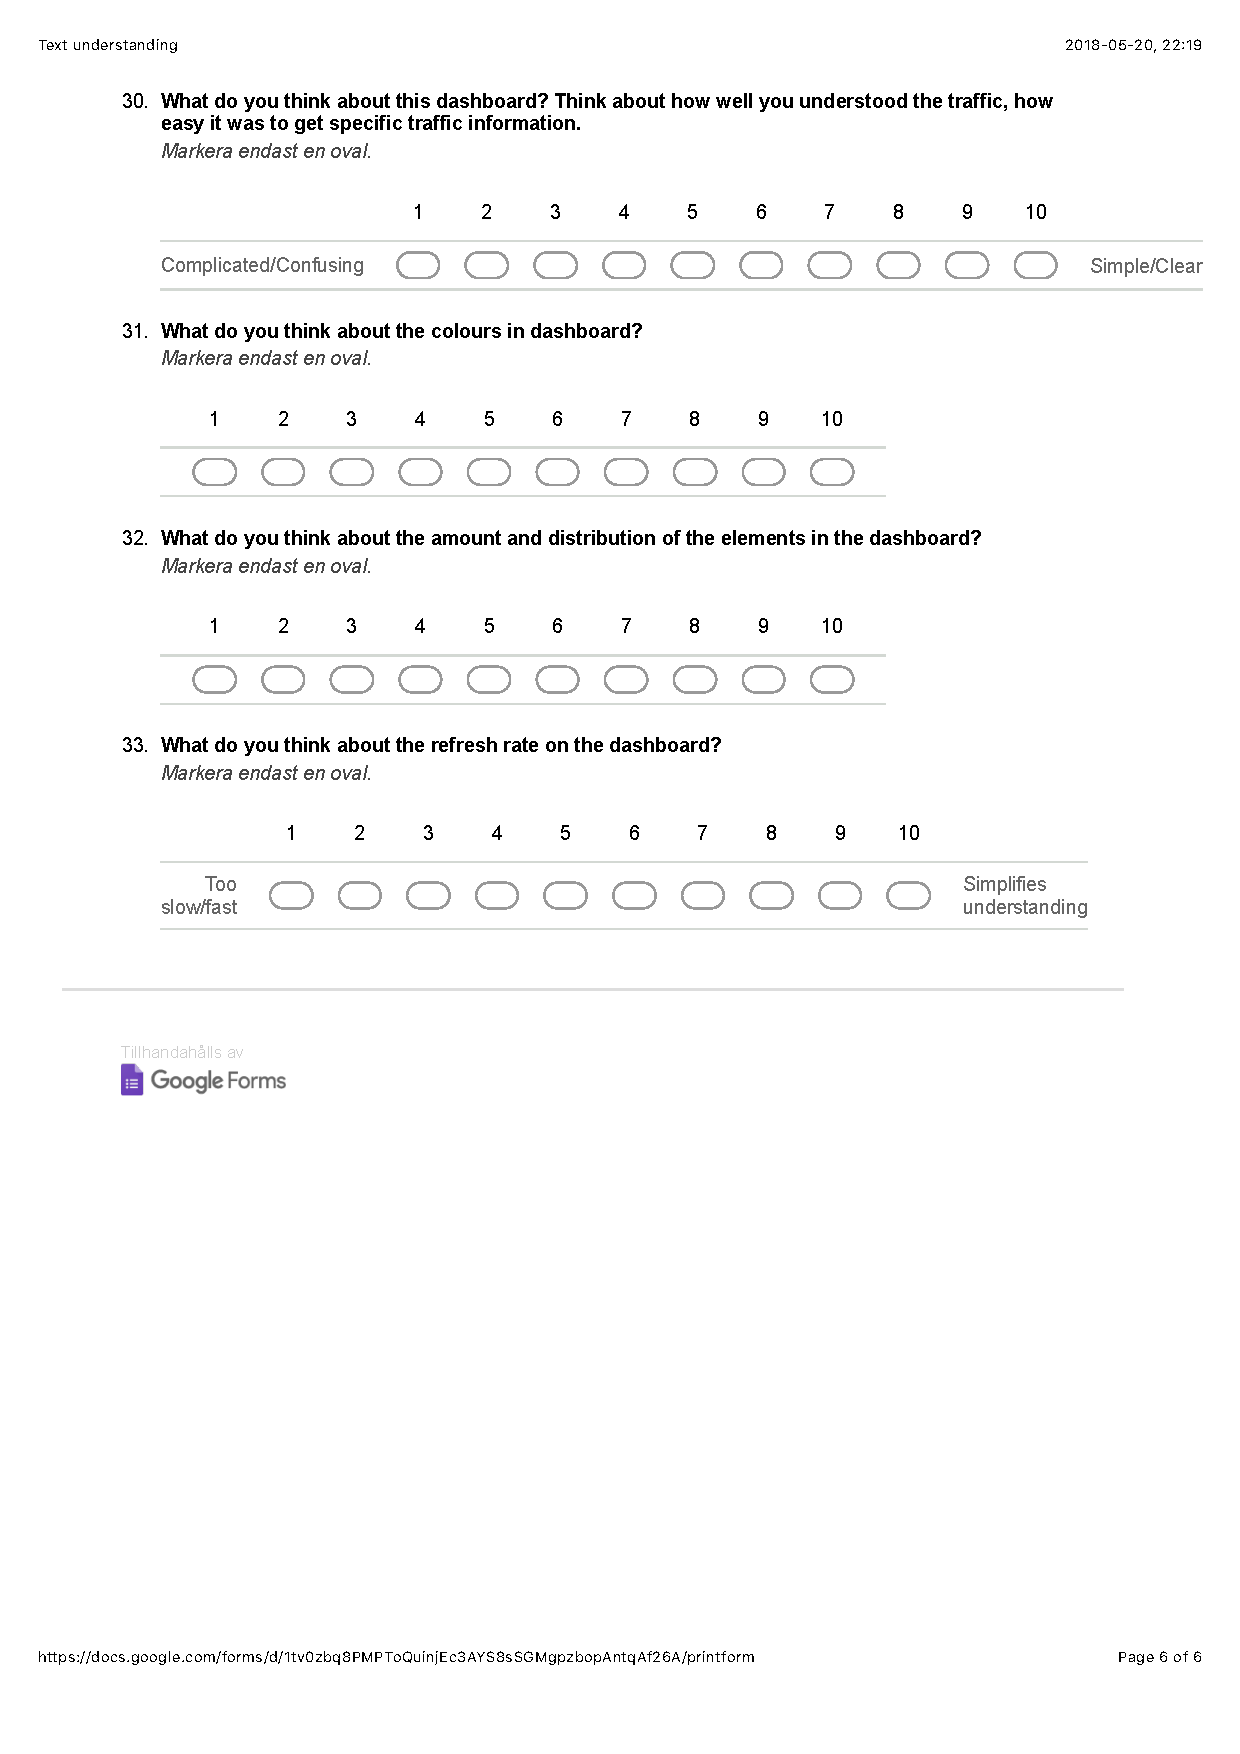
\includegraphics[width=1\textwidth]{TextUnderstanding6.pdf}
\newpage
\section{Resultat av testningsformuläret}
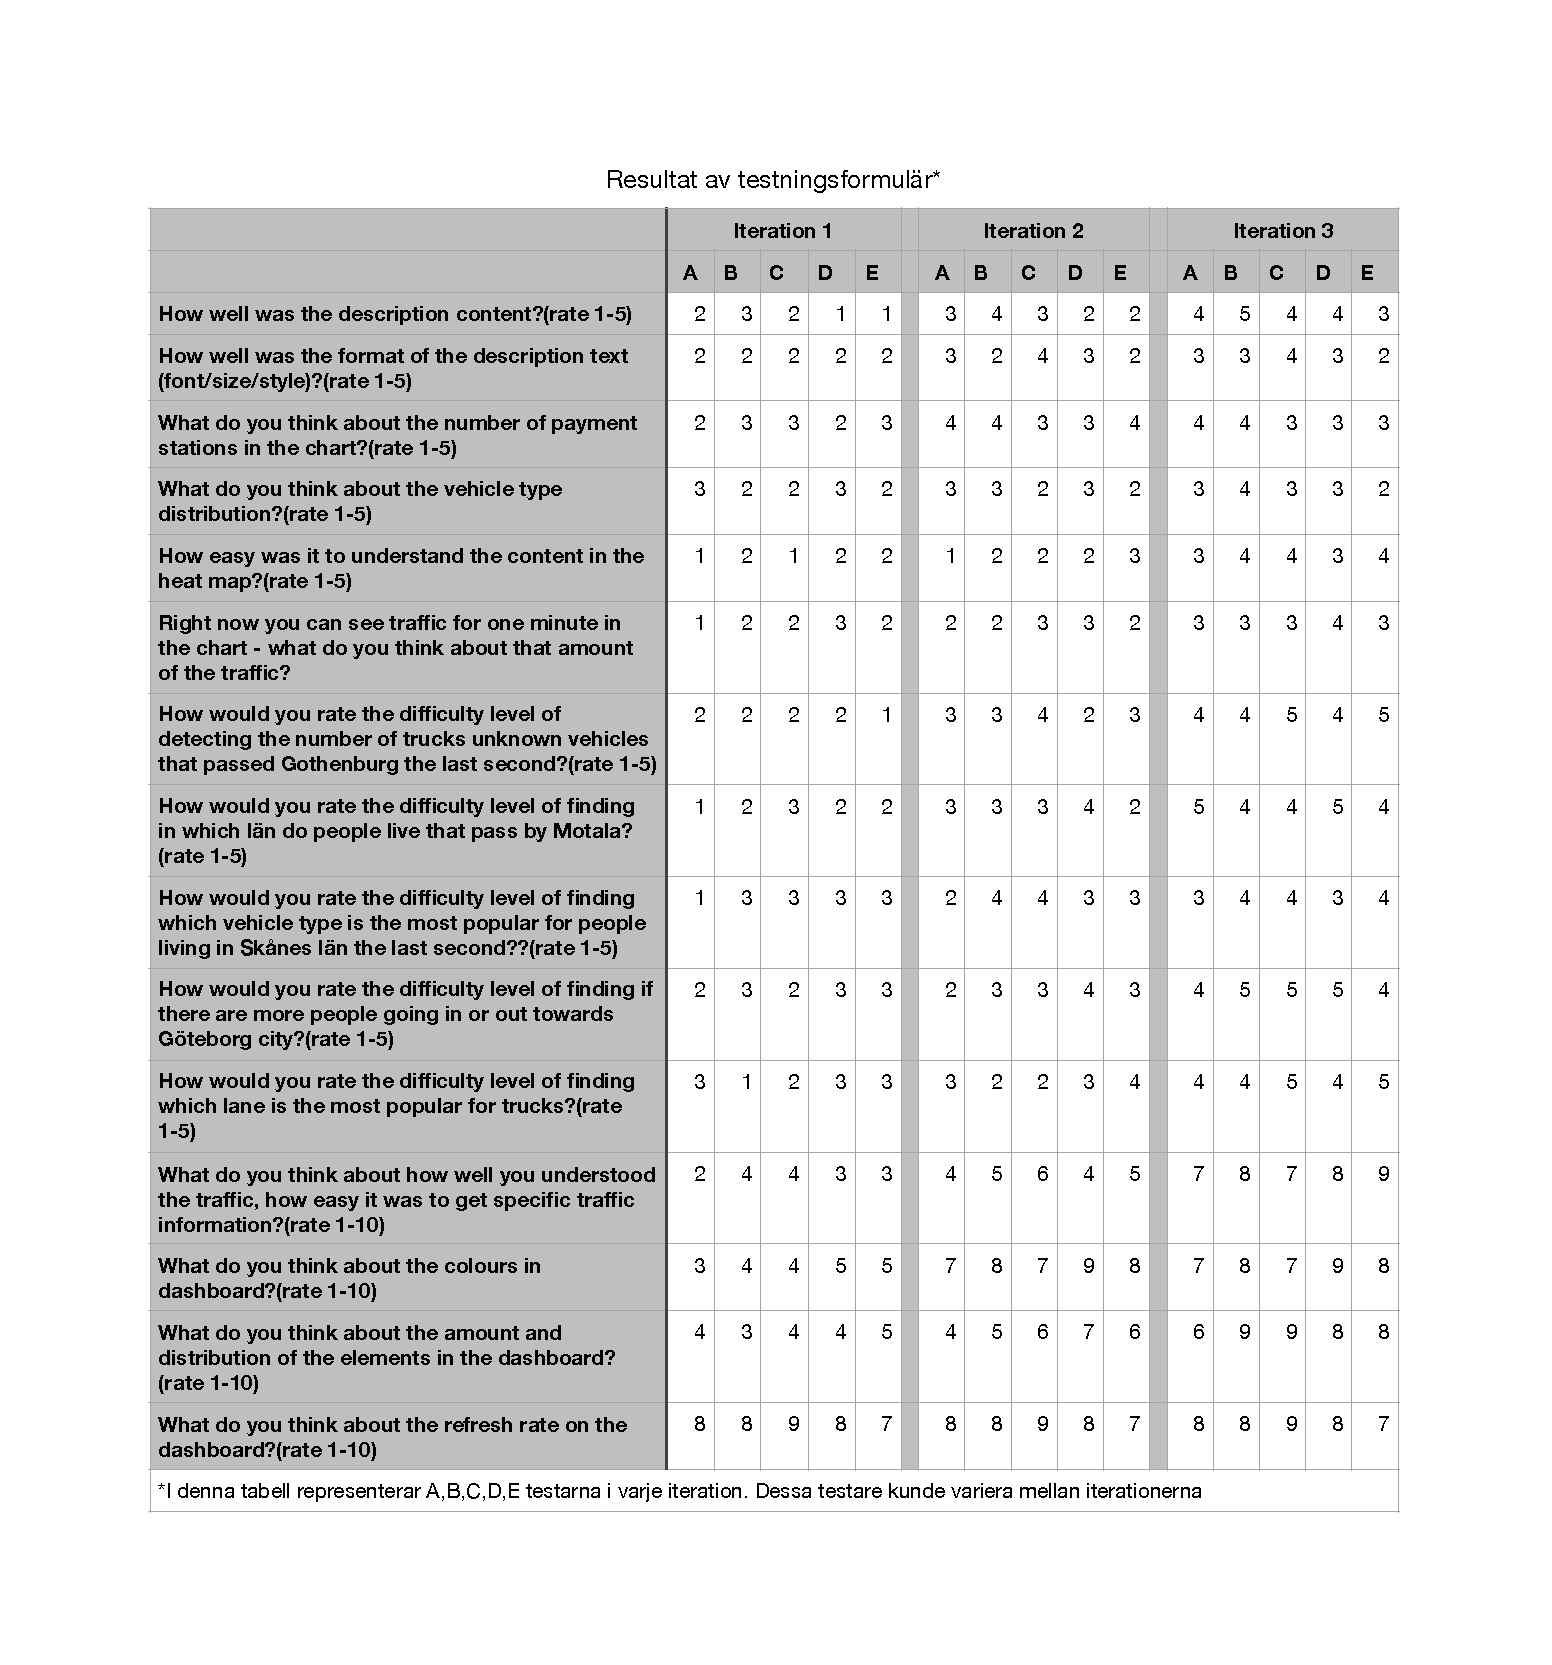
\includegraphics[width=1\textwidth]{TrafficDashboard.pdf}
\newpage
\section{Kibana \textit{dashboard}, slutprodukten}
Följande bilder presenterar slutprodukten av \textit{dashboarden}. De två bilderna sitter ihop men delades upp i två p.g.a. formatering.

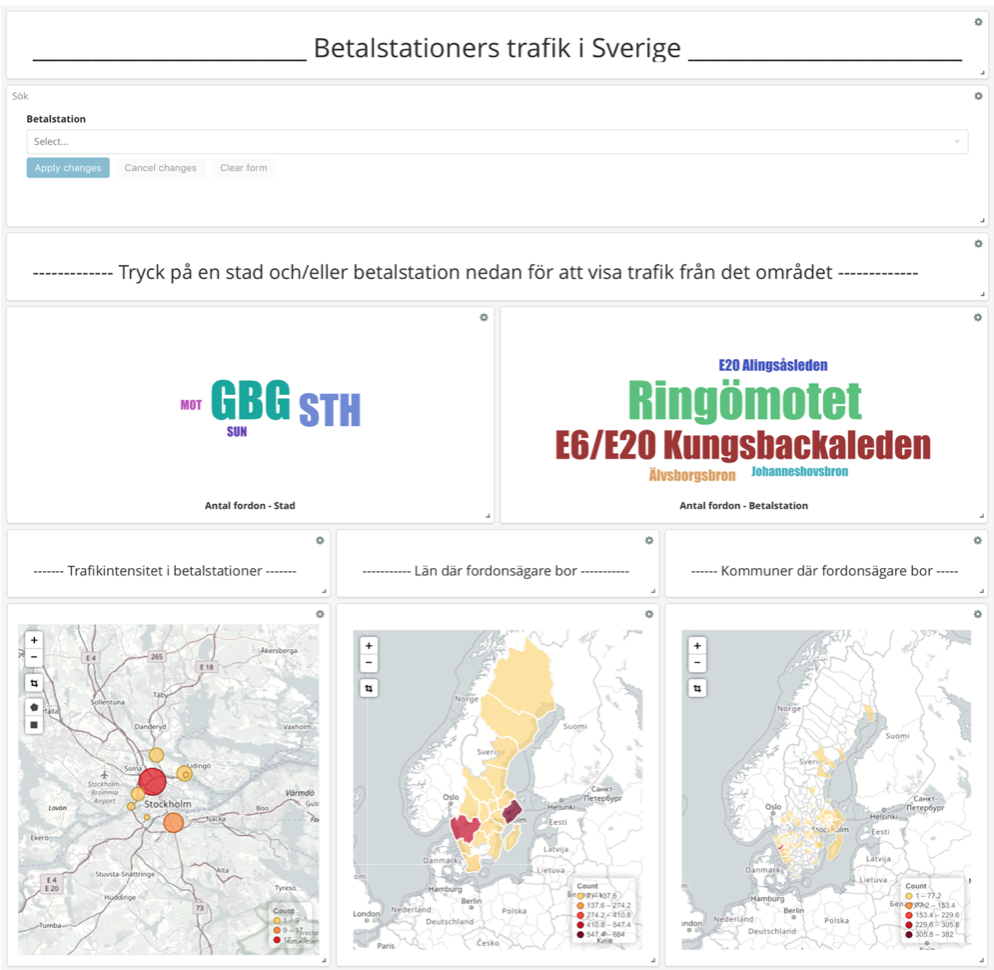
\includegraphics[width=1\textwidth]{Dashboard1}
\newpage
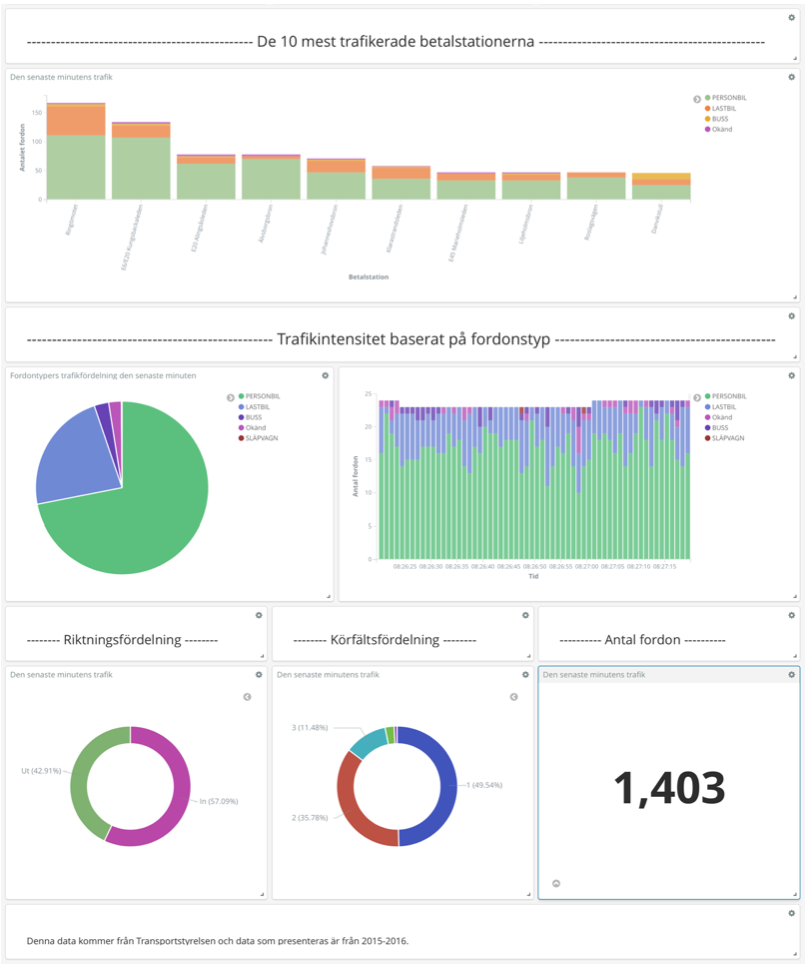
\includegraphics[width=1\textwidth]{Dashboard2}

\end{appendices}

\afterpage{\null\newpage}


\includepdf[pages={-}]{EndPage.pdf}
\end{document}
